\documentclass[12pt,letterpaper,spanish]{article}

\makeatletter  %%%%%% modificacion macro (para puntos en el indice)
\renewcommand*\l@section{\@dottedtocline{1}{1.5em}{2.3em}}
\renewcommand\@dotsep{0.8}
\makeatother %%%%%% fin modificacion macro 

\usepackage[utf8]{inputenc}
\usepackage[spanish]{babel}
\usepackage{times} %Para que salga en times
\usepackage{hyperref}
\hypersetup{colorlinks=true,allcolors=black}
\urlstyle{same}
\usepackage{hypcap}
\usepackage[breakable]{tcolorbox}
\usepackage{dirtytalk}
\usepackage{seqsplit}
\usepackage{wrapfig}
\usepackage{float}
\usepackage{fancyhdr}

 %%%%%%% Packages para hacer las citas
\usepackage[fixlanguage]{babelbib}
\selectbiblanguage{spanish}
\addto\captionsspanish{%
\def\bibname{Referencias}%
\def\tablename{Tabla}%
}
%%%%%%%%%%%%%%%%%%%%%%%%%%%%%%%%%%%%%%%%



\fancyhf{} % sets both header and footer to nothing
\renewcommand{\headrulewidth}{0pt}
% your new footer definitions here


\usepackage{graphicx}
\usepackage{caption}
\usepackage[left=3cm,right=2.5cm,top=3cm,bottom=2.5cm]{geometry}
\usepackage{pdfpages}
\usepackage{amsmath}
\usepackage{longtable}
\usepackage{subfigure} 
\usepackage{ragged2e}
\usepackage{multicol}
\usepackage{xcolor}
\usepackage{rotating}
\usepackage{xcolor}
\usepackage{sectsty}
\usepackage{glossaries}



%Estilo de la página
%\def\arraystretch{1.5}
\renewcommand{\baselinestretch}{1.15}


\chead{\thepage}
%\title{\hfill
\includegraphics[scale=0.6]{logo.png}\vspace{4em}\\
\title{
Pontificia Universidad Católica de Valparaíso\\
Facultad de Ingeniería\\
Escuela de Ingeniería Industrial\vspace{3em}\\
\textbf{Análisis relacional de la pobreza multidimensional en Chile}} %%%%%%%% TITULO INFORME
\author{\LARGE{por}\vspace{1em}\\
\textbf{\LARGE{Maximiliano Muñoz Leiva}}\vspace{1.5mm}\\
\textbf{\LARGE{Matías Negrete Oliva}}\vspace{1.5mm}\\
\textbf{\LARGE{Matías Rodríguez Urtubia}}\vspace{3em}\\
\LARGE{Informe final técnico}\vspace{2em}\\
\LARGE{Prof. Guía: PhD. Sebastián Cea Echenique}\vspace{1em}\\
\LARGE{Prof. Co-Guía: Carlos Erazo Jojot}\vspace{3em}}
\date{\LARGE{8 de julio, 2020}}


\makeglossaries


\newglossaryentry{IPM}
{
        name=\textit{IPM},
        description={índice de pobreza multidimensional}
}
%%%%%%%%%%%%%%%%%%%%%%%%%%%%%%%%%%%%%%%%%%%%%%
\newglossaryentry{INE}
{
        name=\textit{INE},
        description={Instituto Nacional de Estadísticas}
}
%%%%%%%%%%%%%%%%%%%%%%%%%%%%%%%%%%%%%%%%%%%%%%
\newglossaryentry{ONU}
{
        name=\textit{ONU},
        description={Organización de las Naciones Unidas}
}
%%%%%%%%%%%%%%%%%%%%%%%%%%%%%%%%%%%%%%%%%%%%%%
\newglossaryentry{CBA}
{
        name=\textit{CBA},
        description={Canasta básica de alimentos}
}
%%%%%%%%%%%%%%%%%%%%%%%%%%%%%%%%%%%%%%%%%%%%%%
\newglossaryentry{LP}
{
        name=\textit{LP},
        description={Línea de la pobreza por ingresos}
}
%%%%%%%%%%%%%%%%%%%%%%%%%%%%%%%%%%%%%%%%%%%%%%
\newglossaryentry{LPM}
{
        name=\textit{LPM},
        description={Línea de la pobreza multidimensional}
}
%%%%%%%%%%%%%%%%%%%%%%%%%%%%%%%%%%%%%%%%%%%%%%
\newglossaryentry{CEPAL}
{
        name=\textit{CEPAL},
        description={Comisión Económica para América Latina y el Caribe}
}
%%%%%%%%%%%%%%%%%%%%%%%%%%%%%%%%%%%%%%%%%%%%%%
\newglossaryentry{ENUSC}
{
        name=\textit{ENUSC},
        description={Encuesta Nacional Urbana de Seguridad Ciudadana}
}
%%%%%%%%%%%%%%%%%%%%%%%%%%%%%%%%%%%%%%%%%%%%%%
\newglossaryentry{ESCEP}
{
        name=\textit{ESCEP},
        description={Encuesta Seguridad Ciudadana y Evaluación Policial}
}
%%%%%%%%%%%%%%%%%%%%%%%%%%%%%%%%%%%%%%%%%%%%%%

















\begin{document}

%%%%%%%%%%%%%%%%%%%%%%%% para numerar paragraph e indexarlos
\setcounter{tocdepth}{4}
\setcounter{secnumdepth}{4}
%%%%%%%%%%%%%%%%%%%%%%%%%%%%%%%%

\renewcommand{\listtablename}{Lista de Tablas}%%%%%%%%%%% cambio de nombre
\renewcommand{\listfigurename}{Lista de Figuras} %%%%%%% cambio de nombre

\maketitle
\thispagestyle{empty}
\pagestyle{fancy}
\setlength{\parindent}{1cm} %%%%%%%% sangría inicio cada párrafo
\setlength{\parskip}{1em}
%Inicio del documento como tal %%%%%%%%%%%%%%%%%%%%%%%%%%%%%%%%%%%%%%%%%%%%%%%%%%%%%%
%%%%%%%%%%
\newpage
\begin{center}%%%%%% inicio centrado índice, figuras, tablas
\tableofcontents
\clearpage
\listoffigures
\clearpage
%%%%%%%%%%%%%%%%%%%%%% inicio glosario
\glsaddall
\glsaddallunused
\printglossary[type=main]
%%%%%%%%%%%%%%%%%%%% fin glosario
%\listoftables
\clearpage
\end{center}%%%%%%% fin centrado índice, figuras, tablas
%%%%%%%%%%%%%%%%%%%%%%%%%%%%%%%%%%%%%%%%%%%%%%%%%%%%%%%%%%%%%%%%%%%%%%%%%%%%%%%%%%%%%

\section*{Resumen ejecutivo}\addcontentsline{toc}{section}{Resumen ejecutivo} % Max 2 paginas, 5 puntos
La sociedad chilena ha experimentado cambios evidentes en las últimas décadas, disminuyendo significativamente el porcentaje de personas en situación de pobreza por ingresos\footnote{Ver evolución pobreza Encuesta Casen 2006-2017 en \url{http://observatorio.ministeriodesarrollosocial.gob.cl/casen-multidimensional/casen/docs/Resultados_pobreza_Casen_2017.pdf}.}, como resultado del incremento sostenido de los ingresos promedio de los hogares y de las transferencias del Estado\footnote{Ver evolución ingresos de los hogares en \url{https://www.ine.cl/estadisticas/sociales/ingresos-y-gastos/encuesta-suplementaria-de-ingresos}.}. Esto no ha sido un fenómeno aislado, sino que constituye un proceso global de reducción de la pobreza y pobreza extrema\footnote{Ver evolución de pobreza y pobreza extrema en el Mundo 1990-2015 en \url{https://data.worldbank.org/indicator/SI.POV.UMIC?name_desc=false} y \url{https://data.worldbank.org/topic/poverty?name_desc=false} respectivamente.} que, a su vez, ha generado e impulsado la aparición de una gran clase media en Chile \cite{Candia2017RadiografiaPublica} y el Mundo\footnote{Ver evolución de la población de ingresos medios en el Mundo 1990-2018 en \url{https://data.worldbank.org/indicator/SP.POP.TOTL?locations=XP&name_desc=true}.}. A pesar de estos avances, se ha evidenciado un profundo malestar en los últimos años acompañado de crecientes demandas sociales\footnote{Ver noticias ONU en \url{https://news.un.org/es/story/2019/12/1466381}.}, lo que ha dejado de manifiesto que el problema debe entenderse como un fenómeno complejo.  

Desde las propuestas realizadas por Amartya Sen \cite{Sen1976Poverty:Measurement}, los esfuerzos por entender el fenómeno de la pobreza y contar con una medición nueva y apropiada de la misma se han intensificado. En 2007, Sabina Alkire y James Foster, de la Universidad de Oxford, realizaron una propuesta metodológica para medir la pobreza multidimensional de manera agregada, reflejando la prevalencia de la pobreza (cantidad de personas en situación de pobreza) y la distribución conjunta de las privaciones (probabilidad de experimentar carencias simultáneas) \cite{Alkire2007CountingMeasurement}. En 2010, Alkire y Santos tomaron elementos de esta metodología y desarrollaron el Índice de Pobreza Multidimensional (\textit{IPM}) del \textit{PNUD} \cite{Alkire2010AcuteCountries}  que sustituyó el Índice de Pobreza Humana (\textit{IPH}) que \textit{ONU} venía aplicando desde 1997. 

En 2015, el Ministerio de Desarrollo Social y Familia de Chile oficializó cambios metodológicos a los indicadores de pobreza, transitando de una concepción económica a un entendimiento multidimensional de la misma, que la reconoce como un fenómeno complejo. La metodología de la pobreza multidimensional actual recogió la propuesta de Alkire y Foster, desagregando la pobreza en 5 dimensiones (Educación; Salud; Trabajo y seguridad social; Vivienda y entorno; Redes y cohesión social), donde cada una agrupa tres carencias con ponderaciones específicas que al ser sumadas obtienen el indicador general de pobreza multidimensional (\textit{IPM}). En 2016, el sociólogo Pablo Beytía realizó un análisis relacional de la estructura interna de la pobreza multidimensional en base a la Encuesta Casen 2015 \cite{Beytia2016LaMultidimensional}, considerando las carencias del indicador de pobreza multidimensional como una red de correlaciones, es decir, una red de vínculos mutuos entre carencias. Pudo indagar en las dinámicas internas del fenómeno, observar patrones estructurales y calcular pesos estructurales de cada variable y de cada dimensión. 


Considerando el contexto actual de profundas transformaciones sociales, que también han transformado al concepto de familia \cite{OECD2011DoingChanging}, y con las nuevas metodologías para aproximarse holísticamente al fenómeno de la pobreza, el Observatorio Internacional de la Familia de Milán, a través del Programa de Ciencias para la Familia de la PUCV, se encuentra realizando un estudio que tiene por objeto comprender con mayor profundidad las relaciones existentes entre las características y las carencias de las familias. El presente estudio surge con el fin de ser un apoyo al trabajo desarrollado por el Programa de Ciencias para la Familia, mediante una aproximación relacional del análisis de la pobreza. 


La elaboración del estudio se dividió en tres etapas. La primera replicó el análisis relacional de la estructura interna de la pobreza multidimensional desarrollado por Beytía \cite{Beytia2016LaMultidimensional}, considerando esta vez los datos de la Encuesta Casen 2017. En la segunda etapa, a la muestra de hogares pobres multidimensionales se le aplicó la propiedad de descomponibilidad considerando el tipo de hogar, el número de personas que integran el hogar y la zona de residencia del hogar (rural o urbano). A los tipos de hogares se les efectuó un análisis relacional, y al resto de los subgrupos se les realizó un análisis tipológico de las carencias. También se hizo un análisis comparativo con el nivel de ingresos de los hogares. En la última etapa, se recopilaron proyecciones de índices socioeconómicos que permitieron proyectar el indicador de pobreza multidimensional en Chile. Adicionalmente, se realizó un análisis de sensibilidad de las ponderaciones de los indicadores locales del \textit{IPM} (carencias).





 


\newpage
\section{Definición del proyecto} %10 puntos
En esta sección se presenta la descripción del contexto organizacional, la descripción del equipo investigador, la formalización del problema, y el propósito, la justificación y el objetivo del proyecto. También se identifica el sistema de estudio, sus funciones incorporadas y las partes interesadas.

\subsection{Contexto organizacional}
El 6 de diciembre de 2018, en una iniciativa del Pontificio Instituto Teológico Juan Pablo II para las Ciencias del Matrimonio y la Familia, en cooperación con la Universidad Católica San Antonio de Murcia (UCAM) y el Centro Internacional de Estudios de la Familia de Milán (CISF), se creó el Observatorio Internacional de la Familia, cuyo objetivo es analizar el rol que desempeñan las relaciones familiares en la pobreza de las personas\footnote{Ver más información en \url{https://www.vaticannews.va/es/vaticano/news/2018-12/vaticano-observatorio-internacional-familia-pobreza-relaciones.html} y \url{https://www.familymonitor.net/}.}. El Observatorio ha contactado a distintas instituciones académicas y centros de estudio, a los cuales les ha encargado la recopilación de datos nacionales fiables sobre la realidad de las familias en el mundo. Ofrecerá continuamente detalles de la evolución de las condiciones de las familias y comparará las dinámicas familiares en los distintos contextos culturales y políticos de los países, lo cual permitirá enriquecer el análisis de las distintas realidades familiares entendiendo sus complejidades\footnote{Ver información en \url{https://www.vaticannews.va/es/vaticano/news/2018-12/vaticano-observatorio-internacional-familia-pobreza-relaciones.html}.}. 

La primera etapa de la investigación incluyó países de Europa, África y América Latina, y su foco de estudio fue entender cómo la pobreza relacional y económica influye en las dinámicas familiares. El Programa de Ciencias para la Familia, de la Pontificia Universidad Católica de Valparaíso, fue la institución académica seleccionada para realizar la investigación en Chile, disponiendo un equipo interdisciplinario para abordar dicha tarea. El desarollo del presente proyecto fue realizado como una instancia de colaboración al trabajo de este equipo, el cual se encuentra iniciando la segunda etapa de investigación que finaliza en 2021. 

\newpage
\subsection{Descripción organizacional}
El equipo investigador se encuentra constituido por el Director del proyecto y por diez investigadores. En la Figura \ref{equipoInv} se presenta el detalle de los integrantes del equipo y sus respectivas escuelas, institutos o facultades de origen:
\begin{figure}[H]
    \centering
        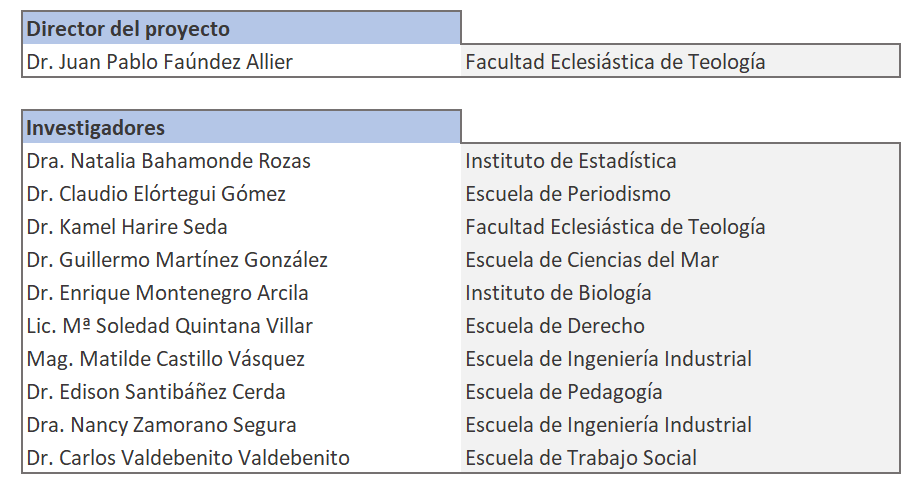
\includegraphics[height=8cm]{Heatmaps/EquipoInvestigador.png}
    \caption{Integrantes Comisión Investigadora. Fuente: Programa de Ciencias para la Familia.}
    \label{equipoInv}
\end{figure}
La diversidad de profesiones y áreas de estudio constituye una de las características principales de este equipo investigador, ya que provee distintas visiones y métodos para aproximarse al objeto de estudio que fue definido como un fenómeno complejo. 

\subsection{Formalización del problema}

En virtud de focalizar la investigación llevada a cabo por el Observatorio Internacional de la Familia, se han formulado una serie de interrogantes, en cuyas respuestas se encuentra el cumplimiento del objetivo inicialmente planteado. La interrogante original del observatorio se puede resumir de la siguiente forma: \textbf{¿Cuál es el rol que desempeñan las relaciones familiares en la pobreza de las personas, desde la perspectiva económica y afectiva?}\footnote{Ver información en \url{https://www.vaticannews.va/es/vaticano/news/2018-12/vaticano-observatorio-internacional-familia-pobreza-relaciones.html}}. 

En la búsqueda de una premisa elaborada que responda a esta pregunta, la comisión investigadora de la PUCV busca desagregar la interrogante para ser abordada desde diferentes aproximaciones disciplinares. En este contexto, nace el interés de la comisión en profundizar la comprensión de las dinámicas relacionales que surgen de la interacción entre los distintos elementos que componen el fenómeno de la pobreza, desde la perspectiva multidimensional. 

Los métodos de medición de la pobreza pretenden identificar al sujeto que se considera pobre y determinar la magnitud social en situación de pobreza. Esto supone, en primer lugar, definir qué se entiende por pobreza y establecer un umbral que actúe como límite diferenciador entre el sujeto pobre y el sujeto no pobre. La medición más difundida de pobreza se expresa mediante una función de ingresos o consumo (por individuo u hogar) que se encuentran bajo un determinado umbral en el que se satisfacen servicios básicos del mercado \cite{Ravallion2011OnPoverty}. En Chile, el umbral de pobreza por ingresos corresponde a la línea de la pobreza, cuantificada a través de una canasta básica de alimentos (CBA) \cite{CEPAL2018MedicionResultados}.

Un aspecto que motiva el consumo, es satisfacer necesidades básicas del individuo. Atkinson plantea que un individuo sufre de exclusión social si no puede satisfacer las necesites básicas respecto a la sociedad a la que pertenece. Pero ser pobre por ingresos no significa estar excluido socialmente y viceversa \cite{AtkinsonExclusionNote}. Resulta pertinente, por consiguiente, incluir una metodología capaz de capturar distintas carencias que se puedan traducir en una privación de las necesidades básicas determinadas por la sociedad; carencias que definirán la estructura de la pobreza.

El índice de pobreza multidimensional (\textit{IPM}) es una agregación de carencias categorizadas por dimensiones, que refleja la prevalencia de la pobreza (cantidad de personas en situación de pobreza) y la distribución conjunta de las privaciones (probabilidad de experimentar carencias simultáneas) \cite{Alkire2007CountingMeasurement}. Entendiendo que cada país tiene características distintas, la aplicación de esta metodología permite elegir y ajustar sus variables y parámetros. De esta manera, las dimensiones, las carencias, las ponderaciones y los umbrales de privación son elegidos por cada sociedad en función de sus requerimientos \cite{Alkire2011UnderstandingsMeasurement}.

El \textit{IPM} de Chile es una función de agregación de 15 carencias distribuidas en 5 dimensiones. Las primeras cuatro dimensiones presentan una ponderación de 22,5\% y la última dimensión pondera 10\%. Las carencias dentro de cada dimensión tienen la misma ponderación. 





\begin{figure}[H]
    \centering
    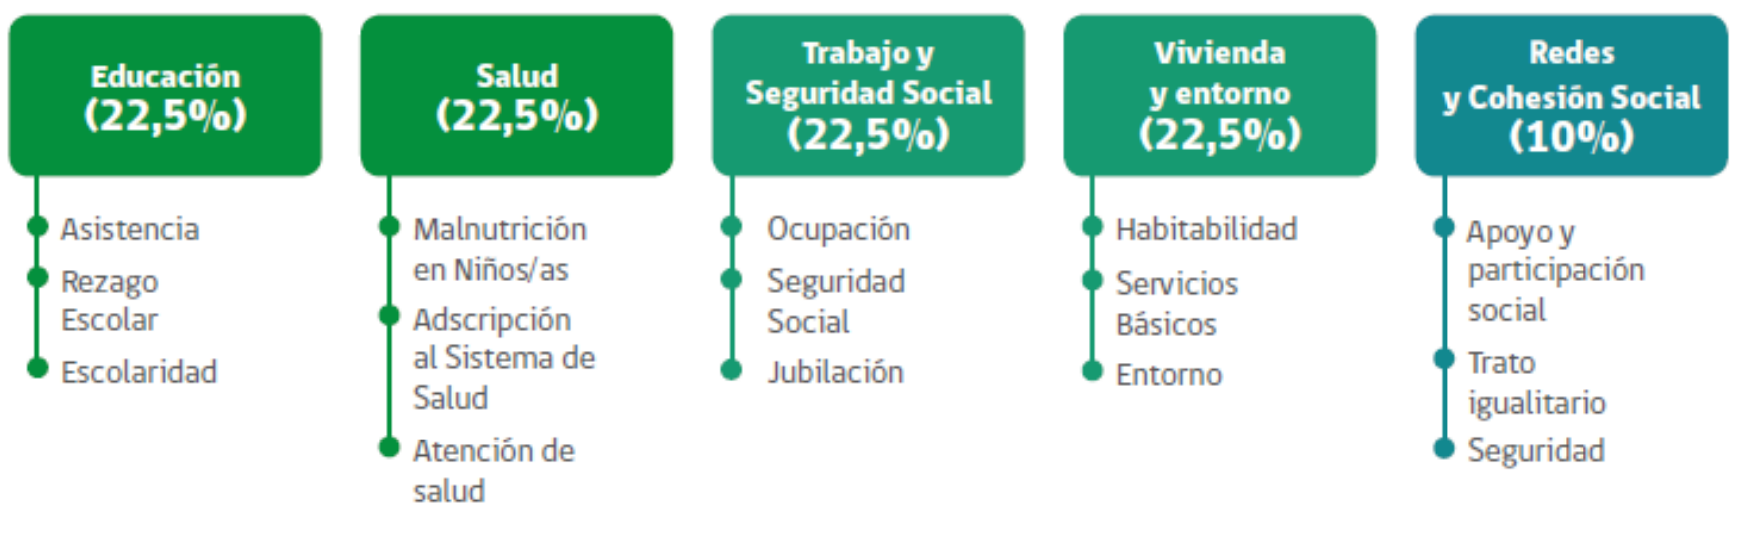
\includegraphics[width=14cm]{Max/multi5d.png}
    \caption{Modelo de medición de la pobreza multidimensional aplicado en Chile, y ponderaciones para el cálculo del IPM. Fuente: Ministerio de Desarrollo Social y Familia.}
    \label{modelo5d}
\end{figure}



En este contexto, el sociólogo chileno Pablo Beytía propuso en 2016 un acercamiento al estudio de la pobreza multidimensional, desde un enfoque relacional. Esto es, ya no desde una perspectiva mecanicista, sino que desde un enfoque sistémico, reconociendo las propiedades emergentes que surgen de las interacciones entre las distintas carencias \cite{Beytia2016LaMultidimensional}.

La comisión de investigadores designada por el Programa de Ciencias para la Familia considera el aporte de Beytía como una propuesta de análisis de gran relevancia para cumplir el objetivo que se le ha designado. En consecuencia, ha levantado los siguientes preguntas de investigación:

\begin{itemize}

    \item ¿Cuáles son las propiedades de la pobreza multidimensional que surgen de la interacción entre los distintos tipos de carencias?

    \item ¿Existen características relacionales entre las carencias que son propias de los diferentes tipos de hogares?

    \item ¿Cómo afecta el número de miembros de cada hogar, su zona de residencia, y su nivel de ingresos en la conformación estructural de sus carencias?

    \item ¿Cuál sería la distribución de la pobreza multidimensional, si a las carencias relacionadas a la dimensión de Redes y cohesión social se les atribuyera la misma relevancia que al resto de las carencias?

    \item ¿Cómo se proyecta la pobreza multidimensional en Chile en el período de crisis sanitaria y social?

\end{itemize}

Ante la necesidad de la comisión de encontrar respuestas, el presente proyecto de investigación busca aportar con información valiosa que contribuya en la comprensión del fenómeno de la pobreza, realizando un estudio desde una perspectiva relacional, para luego complementarlo aplicando criterios de descomponibilidad. Se espera que en su realización se provea a la comisión de los elementos necesarios para el correcto entendimiento de la pobreza multidimensional en la realidad nacional, el cual eventualmente podría permitir focalizar adecuadamente los recursos de las futuras intervenciones sociales que la Iglesia Católica realice en Chile.


\begin{figure}[H]
    \centering
    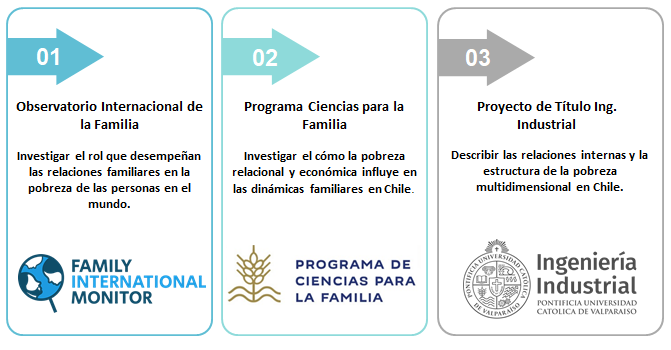
\includegraphics[width=\textwidth]{Max/problema.png}
    \caption{Rol del proyecto en el contexto global de investigación. Fuente: elaboración propia.}
    \label{problema}
\end{figure}



\subsection{Resultados esperados y criterios de aceptación}

%poner las hipótesis y criterios de aceptación

Los criterios de aceptación del estudio realizado se basan, en primera instancia, en la disposición de evidencia que permita aceptar o refutar una serie de afirmaciones que se plantean como respuestas posibles a las interrogantes enunciadas en la sección anterior. Estas afirmaciones pueden ser formalizadas en las siguientes hipótesis:

\begin{itemize}
    \item La aproximación al estudio de la pobreza multidimensional desde la perspectiva relacional permitiría profundizar en el entendimiento de las dinámicas relacionales; dinámicas que surgen de la interacción entre los distintos tipos de carencias. Se plantea la posibilidad de la existencia de factores relacionales que son inadvertidos desde la perspectiva analítica. 
    
    \item La aplicación de la propiedad de descomponibilidad\footnote{Partición de la muestra tomando en cuenta criterios que actúan como filtros de variedad.} al objeto del estudio (hogares pobres multidimensionales) permitiría identificar dinámicas relacionales particulares de cada subgrupo, las cuales estarían determinadas por ciertos factores externos\footnote{Los criterios de descomponibilidad definidos se basan en la clasificación de los factores externos.} a las carencias. Particularmente, se plantea que la diferenciación de los hogares según su estructura (tipos de hogares), según su zona de residencia (rural o urbana) y según su tamaño (número de integrantes) permitiría identificar dinámicas relacionales propias de los subconjuntos diferenciados. 

    \item Existe una relación entre la prevalencia de la pobreza multidimensional y el nivel de ingresos de los hogares pobres multidimensionales. Además, se puede identificar una relación lineal entre el nivel de ingresos y  la intensidad de la pobreza multidimensional (expresada en el índice de pobreza multidimensional \textit{IPM}). 


\end{itemize}  

En segunda instancia, los criterios de aceptación se refieren a la disposición de información que permita prever un escenario probable de la situación actual del fenómeno de la pobreza multidimensional en Chile, así como también del escenario de distribución de la pobreza multidimensional, si se le atribuyera la misma relevancia a las carencias de la dimensión \textit{Redes y cohesión social} que la atribuida al resto de las carencias, para el cálculo del \textit{IPM}.



 













\subsection{Identificación del sistema en estudio}
Si bien el objeto de estudio de este proyecto es la pobreza, esta no se entiende por sí sola, ya que requiere del componente humano para manifestarse. El sistema en estudio, en consecuencia, corresponde a los grupos familiares circunscritos dentro de Chile, cuyas características estructurales determinan la manifestación o no de la pobreza. Resulta relevante recordar que para efectos prácticos y en coherencia con la metodología utilizada, la unidad de análisis es el hogar. Por lo tanto, en este proyecto el hogar constituye la aproximación hacia el estudio de las familias en Chile.

Desde una perspectiva sistémica se entenderá que las familias corresponden a un sistema abierto, donde cada una es un grupo organizado de personas, con identidad propia y en constante interacción, que forman un entramado de relaciones \cite{I.Espinal.2006ElFamilia}. Estas y otras características como la auto-organización, las propiedades emergentes, la retroalimentación, la impredecibilidad y la adaptación, dan cuenta de que la familia también se puede considerar como un sistema complejo.



\newpage
\section{Metodología de ejecución del proyecto} % 10 puntos

La metodología empleada en el desarrollo del proyecto ``Análisis Relacional de la Pobreza Multidimensional en Chile"  se dividió en 3 etapas principales, cada una de las cuales estuvo orientada a comprobar un conjunto determinado de hipótesis y a contribuir en la búsqueda de respuestas a la problemática planteada en la definición del proyecto.

\begin{figure}[H]
    \centering
    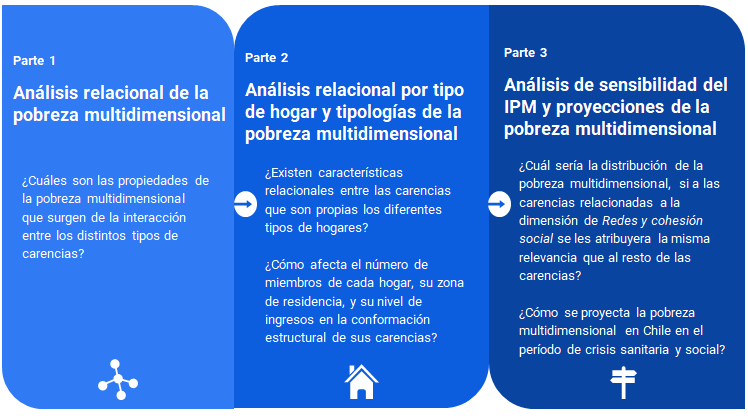
\includegraphics[width=\textwidth]{Max/intro_metodologia.png}
    \caption{División del trabajo metodológico y problemáticas planteadas. Fuente: elaboración propia.}
    \label{intro_metodologia}
\end{figure}






\newpage
\subsection{Metodología análisis relacional de la pobreza multidimensional}

La metodología descrita a continuación tiene por objetivo estudiar las dinámicas relacionales entre las carencias componentes de la pobreza multidimensional. Es decir, en su implementación se buscará entender, desde un enfoque no analítico, la forma en que los distintos tipos de carencias interactúan para conformar el estado de pobreza multidimensional de los hogares en Chile.


\begin{enumerate}
\item \textbf{Obtención de variables} 

Cada hogar se encuentra caracterizado por un conjunto de 15 atributos\footnote{Los atributos que indican la existencia de una carencia son compartidos por todos los miembros que componen un hogar, indistintamente de si alguno de ellos no la posee particularmente.} que indican la existencia o no existencia de cada una de las 15 carencias descritas en el modelo de pobreza multidimensional de 5 dimensiones\footnote{Modelo aplicado en la encuesta CASEN 2017.}. El criterio aplicado para el cálculo del indicador de cada una estas carencias se encuentra disponible en la documentación que dispone el Ministerio de Desarrollo Social y Familia (fig. \ref{tabla_indicadores}; Anexos - fig.\ref{criterios}), y determina la asignación de los valores 1 y 0, en caso de la existencia y la no existencia cada carencia. 


Las variables que requeridas para el análisis relacional corresponden a los indicadores de cada  una de las carencias que componen el índice de pobreza multidimensional (\textit{IPM}), para todos los hogares catalogados como pobres multidimensionales (es decir, aquellos con \textit{IPM} mayor o igual a 22.5\%). Estos indicadores, así como las clasificaciones de los hogares en situación de pobreza dimensional, se encuentran en la base de datos con los resultados de la encuesta CASEN 2017 que dispone el Ministerio de Desarrollo Social y Familia del Gobierno de Chile\footnote{En el documento anexo \ref{descripcion_base_datos} se dispone de una descripción extendida de la base de datos empleada, así como de los atributos asociados a la existencia de cada una de las carencias.}


De forma adicional, se define un conjunto de 5 variables para cada hogar pobre multidimensional de la muestra, cada una de las cuales representa un indicador agregado de las carencias que componen cada una de las 5 dimensiones del \textit{IPM}. Estas variables dimensionales se obtienen de la suma de los indicadores de las carencias que cada una de las dimensiones agrupa.\\

Formalmente, si se considera la definición de los siguientes conjuntos:\vspace{1em}\\
%%%%%%%%%%%%%%%%%%%%%%%%%%%%%%%%%%%%%%%%%%%%%%%%%%%%%%%%%%%%  CONJUNTO HOGARES POBRES multidimensionales
\begin{equation}
\begin{split}
Hogares= hogares\:pobres\:multidimensionales
\end{split}
\end{equation}
%%%%%%%%%%%%%%%%%%%%%%%%%%%%%%%%%%%%%%%%%%%%%%%%%%%%%%%%%%%%%  CONJUNTO DE DIMENSIONES
\begin{equation}
\begin{split}
Dimensiones=\:\{ Salud;\:Educacion;\:Trabajo\: y\: seguridad\:social;\\Vivienda\:y\:entorno;\:Redes\:y\:cohesion\:social\}
\end{split}
\end{equation}
%%%%%%%%%%%%%%%%%%%%%%%%%%%%%%%%%%%%%%%%%%%%%%%%%%%%%%%%%%%%%%% DIMENSION SALUD
\begin{equation}
\begin{split}
Salud=\: \{ Malnutricion\:infantil;\:Atencion;\:Sistema\:de\:salud \}
\end{split}
\end{equation}
%%%%%%%%%%%%%%%%%%%%%%%%%%%%%%%%%%%%%%%%%%%%%%%%%%%%%%%%%%%%%%%%%
\begin{equation}
\begin{split}
Educacion=\: \{ Escolaridad;\:Asistencia;\:Rezago\:escolar\}
\end{split}
\end{equation}
%%%%%%%%%%%%%%%%%%%%%%%%%%%%%%%%%%%%%%%%%%%%%%%%%%%%%%%%%%%%%%%%%
\begin{equation}
\begin{split}
Trabajo y  seguridad  social=\:\{ Ocupacion;\:Seguridad\:social\:;Jubilaciones\}
\end{split}
\end{equation}
%%%%%%%%%%%%%%%%%%%%%%%%%%%%%%%%%%%%%%%%%%%%%%%%%%%%%%%%%%%%%%%%%
\begin{equation}
\begin{split}
Vivienda y entorno=\:\{ habitabilidad;\:Servicios\:basicos;\:Entorno\}
\end{split}
\end{equation}
%%%%%%%%%%%%%%%%%%%%%%%%%%%%%%%%%%%%%%%%%%%%%%%%%%%%%%%%%%%%%%%%%
\begin{equation}
\begin{split}
Redes y cohesion social=\:\{ Trato\:igualitario;\:Seguridad;\:Apoyo\:y\:participacion\:social\}
\end{split}
\end{equation}
%%%%%%%%%%%%%%%%%%%%%%%%%%%%%%%%%%%%%%%%%%%%%%%%%%%%%%%%%%%%%%%%%
\begin{equation}
\begin{split}
Carencias=\:Salud\:\cup\:Educacion\:\cup\:Trabajo\:y\:seguridad\:social\\
\cup\:Vivienda\:y\:entorno\:\cup\:Redes\:y\:cohesion\:social\}
\end{split}
\end{equation}
%%%%%%%%%%%%%%%%%%%%%%%%%%%%%%%%%%%%%%%%%%%%%%%%%%%%%%%%%%%%%%%%%





Las variables obtenidas corresponderán a:


\begin{equation} \label{indicador}
\begin{split}
indicador_{ij}= \begin{cases}
        1;\:si\:hogar\:j\:posee\:carencia\:i\\
        0;\:si\:hogar\:j\:no\:posee\:carencia\:i
        \end{cases}
\end{split}
\end{equation}



\begin{equation} \label{indicador agregado}
\begin{split}
indicador\:dimensional_{zj}=\sum indicador_{ijz};\:z\epsilon Dimensiones
\end{split}
\end{equation}



Las figuras \ref{tabla_indicadores} y \ref{tabla_indicadores_dimensionales} muestran un resumen del criterio de valoración de las variables $indicador_{zj}$ e $indicador\:dimensional_{zj}$ para un hogar \textit{j}, respectivamente. 


\begin{figure}[H]
    \centering
    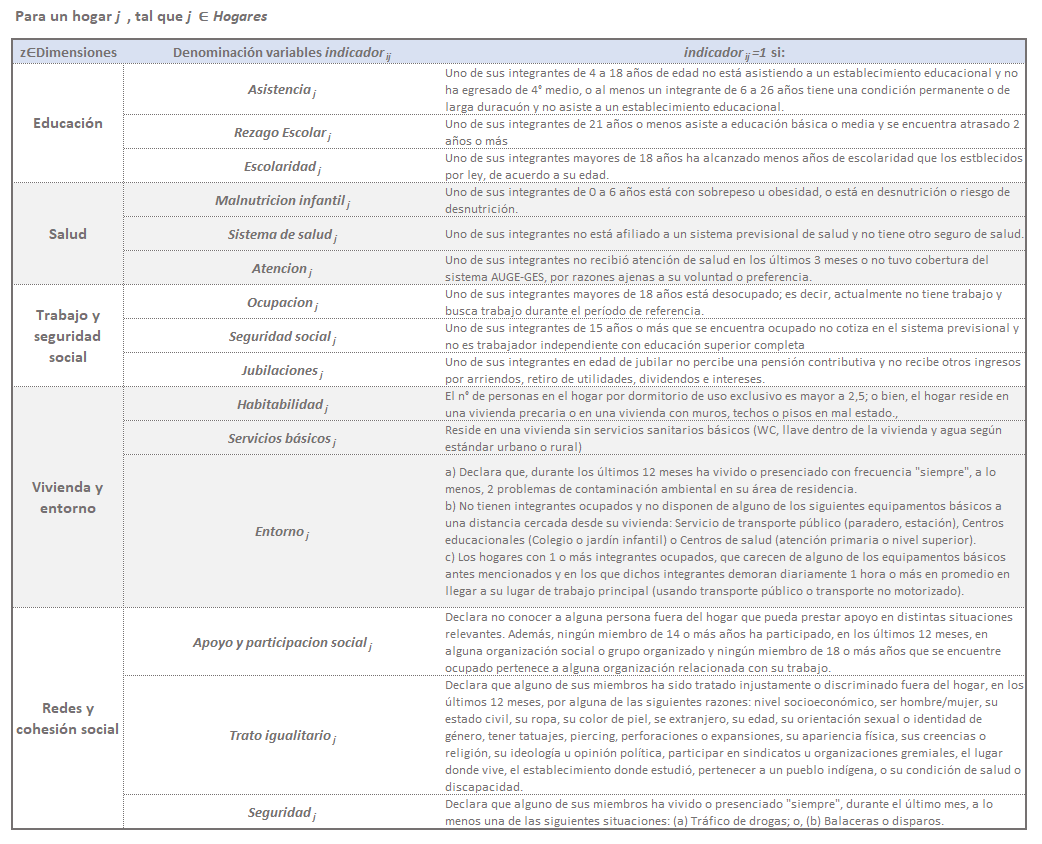
\includegraphics[width=\textwidth]{Max/tabla_indicadores.png}
    \caption{Valorización variables asociadas a carencias. Fuente: elaboración propia.}
    \label{tabla_indicadores}
\end{figure}


\begin{figure}[H]
    \centering
    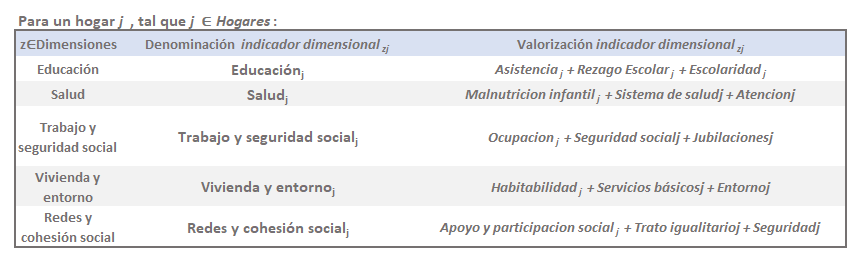
\includegraphics[width=\textwidth]{Max/tabla_indicadores_dimensionales.png}
    \caption{Valorización variables agregadas dimensionales. Fuente: elaboración propia.}
    \label{tabla_indicadores_dimensionales}
\end{figure}
\vspace{2em}


%%%%%%%%%%%%%%%%%%%%%%%%%%%%%%%%%%%%%%%%%%%%%%

\item \textbf{Cálculo de correlaciones entre carencias y dimensiones}

Para cada dupla de indicadores de carencias, se realiza el cálculo del coeficiente phi $\phi$, el cual consiste en una medida de la asociación entre dos o más variables cualitativas. Para este caso en particular, en el que se realiza la comparación de dos variables cualitativas en un dominio de sólo dos categorías (es decir, variables binarias o dicotómicas), el valor del coeficiente phi es equivalente al valor obtenido a través del cálculo del coeficiente de correlación lineal de Pearson \cite{Chedzoy2014Phi-Coefficient}\cite{Chedzoy2006EncyclopediaPhi-coefficient}. El valor del coeficiente phi indicará una mayor intensidad de relación en la medida en que más se acerque en su valor absoluto a 1, y en consecuencia, una menor intensidad de relación en la medida en que el valor se aproxime a 0, asociándose los valores positivos a la co-expresión de ambas variables, y los valores negativos a la co-exclusión.\vspace{1.5em}

Si se consideran como referencias para ejemplificar la obtención del coeficiente phi $\phi$ las carencias $x$ e $y$, se tiene que:
%%%%%%%%%%%%%%%%%%%%%%%%%%%%%%%%%%%%%%%%% carencias x y

\begin{equation}
\begin{split}
indicador_{xj}=\:indicador\:carencia\:x\:del\:hogar\:j\\
indicador_{yj}=\:indicador\:carencia\:y\:del\:hogar\:j
\end{split}
\end{equation}

Luego, para cada hogar pobre multidimensional $j$ se pueden definir las siguientes variables auxiliares:

%%%%%%%%%%%%%%%%%%%%%%%%%%%%%%%%%%%%%%%%% n11 (a)
\begin{equation} \label{n11}
\begin{split}
na_{j}= \begin{cases}
        1;\:si\:indicador_{xj}=\:1\:\ \wedge \:indicador_{yj}=\:1\\
        0;\:e.o.c.
        \end{cases}
\end{split}
\end{equation}
%%%%%%%%%%%%%%%%%%%%%%%%%%%%%%%%%%%%%%%%% n00 (b)
\begin{equation} \label{n00}
\begin{split}
nb_{j}= \begin{cases}
        1;\:si\:indicador_{xj}=\:0\:\ \wedge \:indicador_{yj}=\:0\\
        0;\:e.o.c.
        \end{cases}
\end{split}
\end{equation}
%%%%%%%%%%%%%%%%%%%%%%%%%%%%%%%%%%%%%%%%% n10  (c)
\begin{equation} \label{n10}
\begin{split}
nc_{j}= \begin{cases}
        1;\:si\:indicador_{xj}=\:1\:\ \wedge \:indicador_{yj}=\:0\\
        0;\:e.o.c.
        \end{cases}
\end{split}
\end{equation}
%%%%%%%%%%%%%%%%%%%%%%%%%%%%%%%%%%%%%%%%% n01 (d)
\begin{equation} \label{n01}
\begin{split}
nd_{j}= \begin{cases}
        1;\:si\:indicador_{xj}=\:0\:\ \wedge \:indicador_{yj}=\:1\\
        0;\:e.o.c.
        \end{cases}
\end{split}
\end{equation}


Luego, partir de (\ref{na}), (\ref{nb}), (\ref{nc}) y (\ref{nd}), podemos construir la tabla de contingencia de ambas carencias (fig. \ref{tabla_contingencia}).
%%%%%%%%%%%%%%%%%%%%%%%%%%%%%%%%%%%%%%%%% SUMATORIAS

\begin{equation} \label{na}
\begin{split}
a_{xy}=\sum na_{xy}
\end{split}
\end{equation}

\begin{equation} \label{nb}
\begin{split}
b_{xy}=\sum nb_{xy}
\end{split}
\end{equation}

\begin{equation} \label{nc}
\begin{split}
c_{xy}=\sum nc_{xy}
\end{split}
\end{equation}

\begin{equation} \label{nd}
\begin{split}
d_{xy}=\sum nd_{xy}
\end{split}
\end{equation}\\

%%%%%%%%%%%%%%%%%%

\begin{figure}[H]
    \centering
    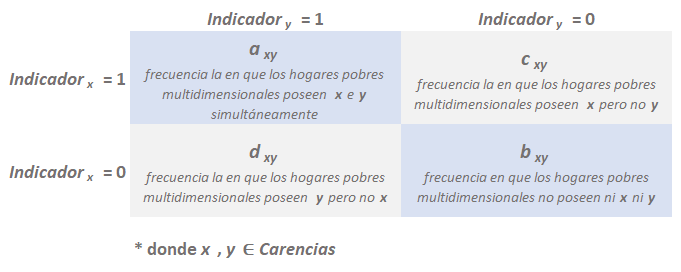
\includegraphics[height=6cm]{Max/tabla_contingencia2.png}
    \caption{Tabla de contingencia carencias $x$ e $y$. Fuente: elaboración propia.}
    \label{tabla_contingencia}
\end{figure}


El coeficiente phi $\phi$ entre las carencias $x$ e $y$ estará dado por:
%%%%%%%%%%%%%%%%%%%%%%%%%%%%%%%%%%%%%%%%  CÁLCULO COEFICIENTE PHI

\begin{equation} \label{calculophi}
\begin{split}
\phi_{xy}=\frac{a_{xy}*b_{xy}-c_{xy}*d_{xy}}{\sqrt{(a_{xy}+c_{xy})(b_{xy}+d_{xy})(b_{xy}+c_{xy})(a_{xy}+d_{xy})}} \: ;\: \phi_{xy} \in [-1;1]
\end{split}
\end{equation}\\

%\( \phi_{xy}=\frac{a*b-c*d}{\sqrt{(a+c)(b+d)(b+c)(a+d)}}\)\vspace{1.5em}\\





Posteriormente, se repite el procedimiento sobre los pares de combinaciones posibles entre las variables dimensionales, empleando como medida de relación el coeficiente de correlación lineal de Pearson $r$, el cual consiste en una medida de relación entre dos variables cuantitativas. Si se consideran los indicadores agregados dimensionales $v_j$ y $w_j$ de un hogar $j$, se tiene que $r_{vw}$ estará dado por la ecuación \ref{formulapearson}.


\begin{equation} \label{formulapearson}
\begin{split}
r_{vw}=\frac{ \sum_{j\in Hogares}^{}(v_j-\bar{v})(w_j-\bar{w}) }{
        \sqrt{\sum_{j \in Hogares}^{}(v_j-\bar{v})^2}\sqrt{\sum_{j\in Hogares}^{}(w_j-\bar{w})^2}}\: ;\: r_{vw} \in [-1;1]
\end{split}
\end{equation}

\vspace{2em}

%%%%%%%%%%%%%%%%%%%%



Los resultados del cálculo de correlaciones, para ambos conjuntos de variables, se grafican posteriormente en un mapa de calor dispuesto como matriz de doble entrada, en cuyas intersecciones se encuentran representadas numéricamente las correlaciones entre dos indicadores de carencia y entre dos indicadores agregados dimensionales, según corresponda.

\vspace{2em}

\item \textbf{Análisis de red de carencias y red de dimensiones}

Las correlaciones obtenidas en el paso anterior son analizadas mediante el modelo de análisis de red ponderada de correlaciones aplicado al estudio de la pobreza multidimensional, el cual fue propuesto por el sociólogo Pablo Beytía \cite{Beytia2016PobrezaChile}. 

Este modelo supone la construcción de una red no dirigida, para la cual el conjunto de nodos representa al conjunto \textit{Carencias} y el conjunto de arcos representa la relación existente entre los distintos pares de carencias. La intensidad de estas relaciones están caracterizadas mediante el peso de los arcos: si la correlación calculada entre dos carencias $x$ e $y$ (nodos) es mayor o igual a $0$, el peso del arco será igual a $\phi_{xy}$; en caso contrario, si la correlación es menor o igual a $0$, el peso del arco será $0$. De forma gráfica, la diferencia entre el peso de distintos arcos se visualizará en su grosor (fig. \ref{modelo_red_carencias}).


Formalmente, dadas las carencias $x$ e $y$, el peso del arco que vincula a ambas carencias $peso_{xy}$ se determina como se indica en la ecuación \ref{pesoarco}.

\begin{equation} \label{pesoarco}
\begin{split}
peso_{xy}= \begin{cases}
        \phi_{xy};\:si\:\phi_{xy}>\:0\\
        0;\:e.o.c.
        \end{cases}
\end{split}
\end{equation}\\




\begin{figure}[H]
    \centering
    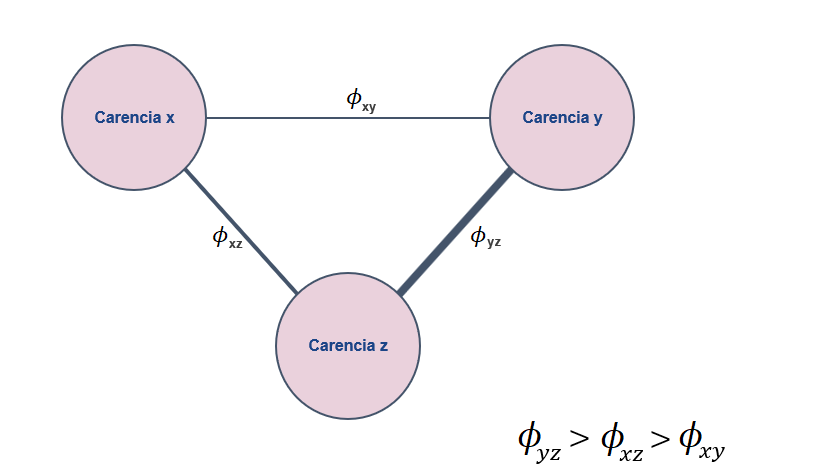
\includegraphics[height=6cm]{Max/redes_phi.png}
    \caption{Modelo red de carencias. Fuente: elaboración propia, basada en modelo de Beytía \cite{Beytia2016PobrezaChile}.}
    \label{modelo_red_carencias}
\end{figure}

Este procedimiento se realiza nuevamente, esta vez representando en los nodos al conjunto \textit{Dimensiones}, en los arcos a las variables agregadas dimensionales, y en el pesos de los arcos los valores positivos obtenidos para el cálculo del coeficiente de Pearson entre las variables agregadas dimensionales (fig. \ref{modelo_red_dimensiones}).


\begin{figure}[H]
    \centering
    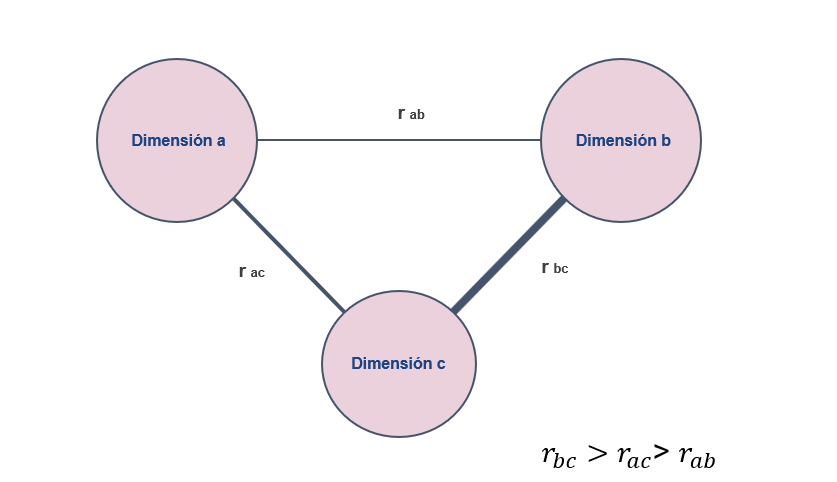
\includegraphics[height=6cm]{Max/redes_pearson.png}
    \caption{Modelo red de dimensiones. Fuente: elaboración propia, basada en modelo de Beytía \cite{Beytia2016PobrezaChile}.}
    \label{modelo_red_dimensiones}
\end{figure}

Posteriormente se efectuará el cálculo de dos medidas de centralidad de la red, las cuales permitirán describir las interacciones relacionales directas e indirectas que existen entre las distintas carencias. Estas medidas corresponden al \textit{grado nodal} de cada carencia, el cual es una medida de centralidad que nos indica la preponderancia de un elemento de la red; y el \textit{grado de intermediación}, el cual indica el grado en que una carencia actúa de enlace entre otras dos carencias que no se encuentran vinculadas directamente entre sí. 


Dada una carencia $x$, se define \textit{grado nodal} del nodo que representa a dicha carencia $s_{x}$ como se indica en la ecuación \ref{gradonodal}\cite{Opsahl2010NodePaths}\cite{CharuC.Aggarwal2011SocialAnalytics}.


\begin{equation} \label{gradonodal}
\begin{split}
s_{x}=\sum_{k\in Carencias\:/\:k\neq x}^{}peso_{xk}
\end{split}
\end{equation}


Dadas las carencias $y$ y $z$, se define $g_{yz}$ como el número de caminos más cortos en la red que conectan los nodos que representan dichas carencias (entendiendo por caminos, a las combinaciones de arcos de la red que permitirían transitar desde una carencia a la otra). Si además consideramos la carencia $x$, se define $g_{yz}(x)$ como el número de caminos más cortos de la red que conectan los nodos de las carencias $y$ y $z$, y que además pasan por el nodo de la carencia $x$. Luego, el \textit{grado de centralidad} $c_{x}$ del nodo que representa a la carencia $x$ se obtendrá como se indica en la ecuación \ref{gradocentral}\cite{Opsahl2010NodePaths}\cite{CharuC.Aggarwal2011SocialAnalytics}.


\begin{equation} \label{gradocentral}
\begin{split}
c_{x}=\sum_{y,z\in Carencias\:/\:y,z\neq x}^{}\frac{g_{yz}(x)}{g_{yz}}
\end{split}
\end{equation}







\end{enumerate}


\subsection{Metodología análisis relacional de la pobreza multidimensional por tipo de hogar y tipologías de la pobreza multidimensional}

La metodología descrita en esta etapa constituye, en primera instancia, una continuación de la ya descrita, esta vez ajustando el enfoque del análisis relacional mediante la división de la muestra de hogares pobres multidimensionales según su clasificación. Posteriormente, la metodología se centra en el análisis de las distintas conformaciones de carencias que caracterizan a los hogares pobres multidimensionales, así como de 2 factores externos al \textit{IPM} que pueden afectar su prevalencia (zona de residencia y número de personas que componen el hogar). Finalmente, se describirá la metodología del análisis comparativo entre el nivel de ingreso de los hogares pobres multidimensionales  y el nivel de pobreza multidimensional, expresada en el \textit{IPM}. 



\subsubsection{Metodología análisis relacional por tipo de hogar}
    

\begin{enumerate}

\item \textbf{Clasificación de hogares}

La clasificación de los hogares se basa en la distinción empleada por el Ministerio de Desarrollo Social y Familia, la cual establece 6 categorías: \textit{Unipersonal}, \textit{Nuclear Monoparental}, \textit{Nuclear Biparental}, \textit{Extendido Monoparental}, \textit{Extendido Biparental} y \textit{Censal}. Con el fin de identificar los criterios de clasificación para cada tipo, es necesario considerar las siguientes definiciones:
\begin{itemize}
    \item \textbf{Hogar:} ``se consideran miembros de un hogar a todas aquellas personas que, siendo residentes de una misma vivienda, pueden tener o no vínculos de parentesco entre sí y habitualmente hacen vida en común, es decir, se alojan y se alimentan juntas. Dicho de otra forma, habitan en la misma vivienda y tienen presupuesto de alimentación común. Un hogar puede estar constituido por una persona o un grupo de personas. Puede ocurrir que en una vivienda exista uno o más hogares. Sin embargo, un hogar no puede ocupar más de una vivienda.
Se excluyen aquellas personas que estuvieron ausentes más de seis meses en el último año, exceptuándose el jefe del hogar y los niños menores de seis meses''. \cite{MDS2019Manual2017}
    
    \item \textbf{Jefe(a) de hogar:} ``es aquel miembro (hombre o mujer) considerado como tal por las otras personas del hogar, ya sea por razones de dependencia económica, parentesco, edad, autoridad o respeto. En todos los hogares se identifica un solo jefe o jefa''. \cite{MDS2019Manual2017}
    
    \item \textbf{Núcleo familiar:} ``es una parte de un hogar (es decir, un subconjunto de sus miembros) y puede estar constituido por una persona sola o un grupo de personas. Comúnmente corresponden a parejas o adultos/as junto a una o más personas que dependen de ellos/as. Puede ocurrir que en un hogar exista uno o más núcleos familiares. Sin embargo, no puede darse que un núcleo familiar esté distribuido en más de un hogar''. \cite{MDS2019Manual2017}
\end{itemize}

En otras palabras, un hogar se define como el conjunto de personas que habitan en la misma vivienda y comparten gastos de alimentación. Al no mediar necesariamente relaciones familiares en su conformación. se define un núcleo familiar como el subconjunto de miembros de un hogar que comparten un tipo de relación más estrecha, en general de parentesco. Bajo esta definición, una vivienda puede albergar a más de un hogar, y un hogar a su vez puede estar constituido por uno o más núcleos. Por el contrario, un núcleo no puede pertenecer a más de un hogar, y un hogar no puede pertenecer a más de una vivienda.


Los tipos de hogares se definen en función de los núcleos familiares que los componen y de las relaciones existentes entre el o la designada como Jefe(a) de hogar y el resto de los miembros del hogar, según los siguientes criterios\footnote{Los criterios de clasificación utilizados para la distinción de los tipos de hogares se basan en la información obtenida de forma directa en la Secretaría Regional Ministerial de Desarrollo Social y Familia Metropolitana del Gobierno de Chile.}:

\begin{itemize}
    \item \textbf{Unipersonal:} hogares conformados por solo un integrante.
    
    \item \textbf{Nuclear Monoparental:} hogares conformados por dos o más personas pertenecientes a un mismo núcleo, y cuyo Jefe(a) de hogar no tiene una relación de pareja (formal o informal) con otro miembro del hogar (de distinto o igual sexo).
    
    \item \textbf{Nuclear Biparental:} hogares conformados por dos o más personas pertenecientes a un mismo núcleo, y cuyo Jefe(a) de hogar tiene una relación de pareja (formal o informal) con otro miembro del hogar (de distinto o igual sexo).
    
    \item \textbf{Extendido Monoparental:} hogares conformados por más de un núcleo (donde al menos uno está conformado por dos o más miembros), y cuyo Jefe(a) de hogar no tiene una relación de pareja (formal o informal) con otro miembro del hogar (de distinto o igual sexo).
    
    \item \textbf{Extendido Biparental:} hogares conformados por más de un núcleo (donde al menos uno está conformado por dos o más miembros), y cuyo Jefe(a) de hogar tiene una relación de pareja (formal o informal) con otro miembro del hogar (de distinto o igual sexo).
    
    \item \textbf{Censal:} hogares conformados por dos o más personas sin relaciones familiares (cada persona constituye un núcleo familiar diferente).
\end{itemize}

A continuación ilustrará el criterio de clasificación mediante un ejemplo sencillo:

\begin{itemize}
    \item En una casa (\textit{vivienda}) residen 2 estudiantes universitarios: Magdalena y Domingo. Debido a que no comparten un presupuesto de alimentación (i.e. realizan las compras de víveres por separado),  cada uno de ellos constituye un hogar independiente. Al ser cada uno de ellos los únicos miembros de sus hogares respectivos, ambos hogares serían del tipo \textbf{unipersonal}.
    
    \item Eventualmente, los estudiantes deciden empezar a compartir los gastos de alimentación para aprovechar los beneficios de unir ambos presupuestos.  Desde ese momento pasan a constituir un único hogar. Sin embargo, debido a que la relación que los vincula se basa solo en un motivo económico (y no de dependencia o parentesco), cada uno de ellos constituye un núcleo familiar independiente. Luego, al estar el hogar conformado por 2 personas, cada una de las cuales constituye un núcleo diferente, este se clasificaría como \textbf{censal}.
    
    \item Con el tiempo ambos estudiantes estrechan su relación, inician una relación de pareja y tienen un hijo. Ahora se puede decir que, al existir un vínculo de familiaridad y dependencia entre ellos (y su hijo), los tres conforman un solo núcleo familiar, y un sólo hogar. Magdalena es quien, en general, toma las decisiones del hogar, por lo que se le puede identificar como \textit{jefa de hogar}. Al tener Magdalena una pareja dentro del hogar (Domingo), y debido a que los tres miembros del hogar conforman un solo núcleo, el hogar se clasificaría como \textbf{nuclear biparental}.
    
    \item Luego de un par de años, Magdalena y Domingo deciden terminar su relación, por lo que Domingo se traslada a otra residencia (deja, por lo tanto, de pertenecer al hogar y al núcleo familiar). Magdalena y su hijo aún conforman un hogar y un núcleo. Ahora bien, debido a que ella, como jefa de hogar no tiene una relación de pareja con otro miembro del hogar, junto a su hijo conforman un hogar clasificado como \textbf{nuclear monoparental}. 
    
    \item Con el fin de mejorar su economía familiar, Magdalena comienza a arrendarle una habitación de huéspedes a sus amiga Inés y Sonja, y juntas deciden además compartir gastos de alimentación (por lo tanto conforman, junto al hijo de Magdalena, un sólo hogar). Al no mediar una relación de parentesco o dependencia entre ellas, Inés y Sonja constituyen, cada una de ellas, un núcleo familiar independiente, y debido a que Magdalena (jefa de hogar) no tiene una relación de pareja con otro miembro del hogar, el hogar que constituyen es del tipo \textbf{extendido monoparental}.
    
    \item Finalmente, Magdalena estrecha su relación con Sonja y comienzan una relación de pareja. Sonja desde entonces pasa a constituir parte del núcleo familiar de Magdalena. El hogar entonces queda constituido por dos núcleos: el de Magdalena, su hijo y Sonja, y el de Inés. Al tener Magdalena (jefa de hogar) una pareja dentro del hogar, los cuatro conforman un hogar \textbf{extendido biparental}.
    
\end{itemize}

\vspace{2em}


\item \textbf{Análisis de red de carencias por tipo de hogar}

Para cada subconjunto de la muestra particionada según la clasificación por tipo de hogar definida en el punto anterior, se efectuará el cálculo del coeficiente $\phi$ entre cada dupla de carencias y, posteriormente, el análisis de red de carencias, siguiendo el mismo procedimiento empleado anteriormente para el conjunto total de hogares pobres multidimensionales.

\end{enumerate}


%%%%%%%%%%%%%%%%%%%%%%%%%%%%%%%%%%%%%%%%%%%%%%%%%%%%%%%%%%%%%%%%%%%%%%%%%%%%%%


\subsubsection{Metodología análisis tipológico}


\begin{enumerate}
\item \textbf{Cálculo del \textit{IPM} por hogar}

Para cada hogar clasificado como pobre multidimensionalmente se calculará el \textit{IPM}\footnote{Si bien la base de datos de la encuesta CASEN 2017 dispuesta por el Ministerio de Desarrollo Social y Familia incluye la clasificación de cada hogar en \textit{pobre} y \textit{no pobre} respecto a la pobreza multidimensional, no incorpora el valor calculado para el \textit{IPM}}, según la ponderación del modelo de 5 dimensiones (fig. \ref{ponderaciones}).

\begin{figure}[H]
    \centering
    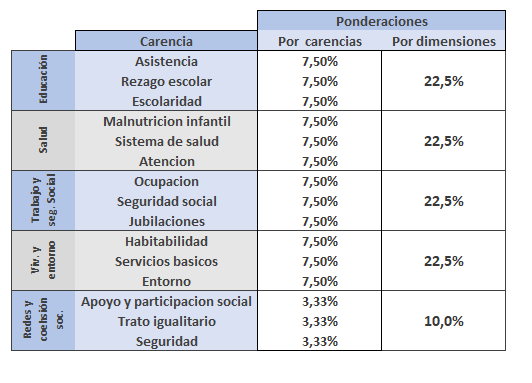
\includegraphics[height=9cm]{Max/ponderaciones.png}
    \caption{Ponderaciones de carencias y dimensiones para el cálculo del \textit{IPM} - CASEN 2017. Fuente: elaboración propia.}
    \label{ponderaciones}
\end{figure}

\vspace{2em}

\item \textbf{Determinación tipologías}


 Se calculará la frecuencia del conjunto de combinaciones posibles entre las 15 carencias del modelo de pobreza multidimensional de 5 dimensiones, para los hogares pobres multidimensionales registrados en la encuesta CASEN 2017. Cada una de estas combinaciones configura una tipología específica de la estructura de carencias, la cual será caracterizada por un \textit{IPM} asociado.
 
 \vspace{2em}

\item \textbf{Determinación tipologías por factores externos}

El procedimiento de determinación de tipologías y análisis de frecuencia se realizará nuevamente, esta vez  aplicando el principio de descomponibilidad a través de una partición de los datos según los siguientes factores externos:

    \begin{itemize}
        \item  \textbf{Zona} (de residencia), pudiendo los hogares pertenecer a las categorías \textit{rural} y \textit{urbano}. 
        \item \textbf{Número de integrantes} que conforman el hogar, sin considerar al personal de servicio doméstico puertas adentro. 
    \end{itemize}
\end{enumerate}


\subsubsection{Metodología análisis comparativo con nivel de ingresos}

La metodología descrita a continuación busca comprender la relación entre los niveles de ingresos de los hogares pobres multidimensionales y sus estructuras de carencias, empleando como medida de referencia la línea de la pobreza por ingresos (\textit{LP}). 

La línea de la pobreza es definida por la \textit{CEPAL} como la representación de un valor monetario en el que se considera el costo de adquisición de una canasta básica de alimentos (\textit{CBA})\footnote{La \textit{CBA} se construye, según la \textit{CEPAL},  ``de manera que satisfaga los requerimientos calóricos promedio de la población, mediante una estructura de bienes y precios proveniente de las pautas de consumo observadas en un grupo de referencia y ajustada de manera que cuente con equilibrios nutricionales básicos''\cite{CEPAL2018MedicionResultados}.}, expresado sobre la base de la relación entre el gasto total y el gasto en alimentos \cite{CEPAL2018MedicionResultados}. La medición de la pobreza por ingresos, se determina mediante la comparación entre el ingreso percibido del hogar y el ingreso mínimo necesario para satisfacer las necesidades básicas que están representadas en la \textit{CBA}, siendo el valor de \textit{LP} el ingreso necesario para financiar la \textit{CBA}. La línea de la pobreza es calculada regularmente por el Ministerio de Desarrollo Social y Familia, y en su determinación se realiza además un ajuste en función del número de personas que integran el hogar, debido a que se supone la existencia de economías de escala para ciertos gastos. En consecuencia, todos aquellos hogares cuyos niveles de ingresos sean inferiores a \textit{LP}, serán catalogados como pobres por ingresos \cite{CEPAL2018Medicion2017}.


Ante la inexistencia de una metodología oficial del Gobierno de Chile que defina una estratificación socio-económica, el centro de estudios e investigación privado \textit{Libertad y Desarrollo} realizó el año 2019 una propuesta de clasificación socio-económica expresada en términos del nivel de ingresos relativo a la línea de la pobreza, con el fin de acercarse al marco metodológico empleado por el Banco Mundial \cite{LibertadyDesarrollo2019HaciaChile}. Esta propuesta considera 6 categorías socio-económicas, definidas como se indica en la fig. \ref{clasld}.


\begin{figure}[H]
    \centering
    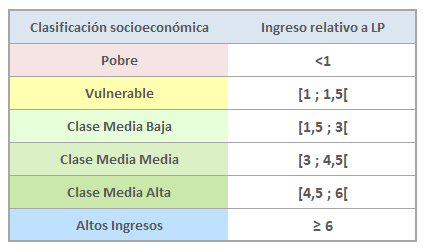
\includegraphics[height=6cm]{Max/clasificacion_ld.png}
    \caption{Propuesta \textit{Libertad y Desarrollo} de clasificación socio-económica por ingreso, expresado en términos de \textit{LP}. Fuente: elaboración propia, a partir de información dispuesta por \textit{Libertad y Desarrollo} \cite{LibertadyDesarrollo2019HaciaChile}. }
    \label{clasld}
\end{figure}



\begin{enumerate}
    


\item \textbf{Definición variable relativa de ingreso}

Para simplificar el análisis respecto al ingreso de los hogares, este se realizará empleando el indicador relativo del ingreso ajustado del hogar respecto a la línea de la pobreza. Para cada hogar $j$, el indicador relativo $ingreso\:relativo_{j}$ se define como el cociente entre el producto del ingreso \textit{per cápita} del hogar corregido (\textit{ypc}) y el número de personas de componen el hogar $n_{j}$,  y la línea de pobreza (\textit{LP}) ajustada según el número de personas que componen el hogar $LP_n$. Se emplearán como referencia para la \textit{LP} los valores calculados por el Ministerio de Desarrollo Social y Familia en el mes de noviembre de 2017 (fig. \ref{LPLPE}).

\begin{equation} \label{calculophi}
\begin{split}
ingreso\:relativo_{j}=\frac{ypc_{j}*n_{j}}{LP_{n}}\: ;\:n=n_{j}
\end{split}
\end{equation}\\

%\( \phi_{xy}=\frac{a*b-c*d}{\sqrt{(a+c)(b+d)(b+c)(a+d)}}\)\vspace{1.5em}\\



\begin{figure}[H]
    \centering
    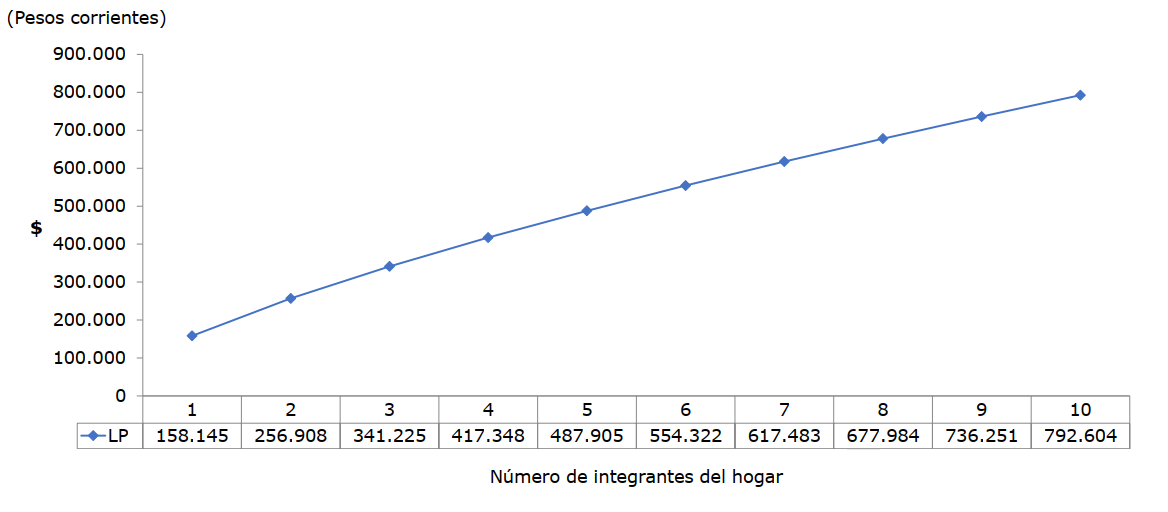
\includegraphics[width=\textwidth]{Max/linea_pobreza.png}
    \caption{Valor de la línea de la pobreza ($LP_n$) en función del número de integrantes del hogar $n$, Noviembre 2017. Fuente: Ministerio de Desarrollo Social y Familia}
    \label{LPLPE}
\end{figure}

\vspace{2em}

\item \textbf{Clasificación hogares pobres multidimensionales por estrato socio-económico}

Los hogares pobres multidimensionales se clasificarán en distintos intervalos socio-económicos, según el criterio propuesto por \textit{Libertad y Desarrollo}, con el objetivo de identificar el grado de contribución de cada categoría al total de hogares pobres multidimensionales.

\vspace{2em}


\item \textbf{Comparación indicador ingreso relativo e \textit{IPM}}

Los valores obtenidos para el indicador relativo de ingreso de cada hogar pobre dimensional se grafican en función del índice de pobreza multidimensional, a través de un diagrama de dispersión. El grado de relación entre ambas variables se medirá empleando para ello el coeficiente de correlación lineal de Pearson. 

\vspace{2em}


\item \textbf{Comparación indicador ingreso relativo y padecimiento de carencias}

Con el fin de determinar la relación particular entre el padecimiento de una carencia del modelo de 5 dimensiones y el nivel de ingreso de los hogares, se analizará la distribución del indicador relativo de ingreso para cada conjunto de hogares pobres multidimensionales que padezcan una carencia en particular. 

\end{enumerate}




\newpage
\subsection{Metodología análisis de sensibilidad del \textit{IPM} y proyecciones de la pobreza multidimensional}


\subsubsection{Metodología análisis de sensibilidad del \textit{IPM}}


Se recalculará el índice de pobreza multidimensional de los hogares de la muestra CASEN 2017, esta vez ponderando cada indicador de carencias de igual forma (fig. \ref{ponddos}). 

\begin{figure}[H]
    \centering
    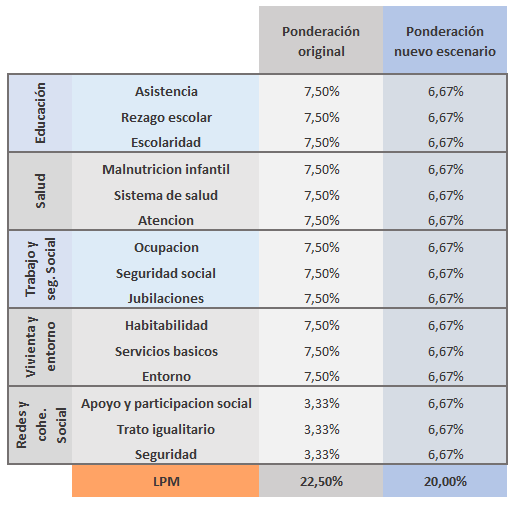
\includegraphics[height=10cm]{Max/ponderaciones_sensib.png}
    \caption{Ponderación de carencias para análisis de sensibilidad del \textit{IPM}. Fuente: elaboración propia.}
    \label{ponddos}
\end{figure}

La línea de la pobreza multidimensional (\textit{LPM}) empleada originalmente, se determinó en función de la ponderación del \textit{IPM} en hogares que padecen un mínimo de tres carencias pertenecientes a las dimensiones \textit{Educación}, \textit{Salud}, \textit{Vivienda y entorno} y \textit{Trabajo y seguridad social}, correspondiente a un 22.5\%. En lineamiento con lo anterior, la línea de pobreza dimensional definida para el nuevo escenario, corresponderá a la ponderación del \textit{IPM} de los hogares que padecen un mínimo de tres carencias, siendo estas pertenecientes a cualquiera de las cinco dimensiones (es decir, incluyendo la dimensión \textit{Redes y cohesión social}), correspondiente a un 20\%. 

Habiendo obtenido una nueva distribución de la pobreza multidimensional, se realizará nuevamente un análisis reticular de las carencias de los hogares pobres multidimensionales.




\subsubsection{Metodología proyecciones de la pobreza multidimensional}
Se realizará una proyección del \textit{IPM} promedio y de la prevalencia de la pobreza multidimensional para el segundo semestre de 2020. Esta se construirá en base a la proyección de la incidencia las carencias \textit{Ocupación} y \textit{Seguridad}, bajo el supuesto \textit{ceteris paribus} respecto a la medición del resto de carencias en la encuesta CASEN 2017. En otras palabras, se trabajará bajo el supuesto de que para ninguna de las carencias contempladas en el modelo trabajado (exceptuando \textit{Ocupación} y \textit{Seguridad}), han existido variaciones significativas en los últimos tres años. 

\begin{enumerate}

    \item \textbf{Proyección prevalencia Ocupación}
    
    Para la proyección de la frecuencia de la carencia \textit{ocupación} en los hogares, se asumirá la existencia de una relación directamente proporcional entre la tasa de desocupación estimada por el \textit{INE}\footnote{El Instituto Nacional de Estadísticas emite periódicamente boletines con la estimación de la tasa desocupación, los cuales están disponibles en el sitio \url{https://www.ine.cl/estadisticas/sociales/mercado-laboral/ocupacion-y-desocupacion}}. Si definimos $f.carencia ocupacion$ como la frecuencia porcentual de hogares que padecen la carencia de \textit{ocupación}, $t. desocupacion$ como la tasa de desocupación estimada por el \textit{INE}, $t$ como el período de referencia para el cálculo, y $t+h$ como el período sobre el cual se realiza la proyección, la proyección de la frecuencia de la carencia \textit{ocupación}, en el período $t+h$ estará dada por:
    
    \begin{equation}\label{calculo_proyeccion_ocupacion}
        \begin{split}
            f.carencia\:ocupacion_{t+h}=\frac{t.desocupacion_{t+h}*f.carencia\:ocupacion_t}{t.desocupacion_t}\\
        \end{split}
    \end{equation}
    
    \vspace{2em}
    
    
    
    
    \item \textbf{Proyección prevalencia Seguridad}
    
    La proyección de la carencia \textit{seguridad} se realizará de forma similar a la de \textit{ocupación}, pero empleando como medida referencial el índice de \textit{percepción del aumento de la delincuencia y exposición frente al delito} \footnote{El Instituto Nacional de Estadísticas emite anualmente un boletín con los resultados de la Encuesta Nacional Urbana de Seguridad Ciudadana (ENUSC), la cual incorpora el indicador de \textit{Percepción del aumento de la delincuencia y exposición frente al delito}. Los resultados de la ENUSC se encuentran disponibles en el sitio \url{https://www.ine.cl/estadisticas/sociales/seguridad-publica-y-justicia/seguridad-ciudadana}}. De esta forma, si definimos $f.carencia seguridad$ como la frecuencia porcentual de hogares que padecen la carencia de \textit{seguridad}, $i. seguridad$ como la estimación de la percepción del aumento de la delincuencia y exposición frente al delito realizada por el \textit{INE}, $t$ como el período de referencia para el cálculo, y $t+h$ como el período sobre el cual se realiza la proyección, la proyección de la frecuencia de la carencia \textit{seguridad}, en el período $t+h$ estará dada por \ref{calculo_proyeccion_seguridad}.
    
    \begin{equation}\label{calculo_proyeccion_seguridad}
        \begin{split}
            f.carencia\:seguridad_{t+h}=\frac{i.seguridad_{t+h}*f.carencia\:seguridad_t}{i.seguridad_t}\\
        \end{split}
    \end{equation}
    
    
    \item \textbf{Proyección IPM}


Para la proyección del \textit{IPM} en el período $t+h$ se empleará el método \textit{Montecarlo}. Este corresponde a una metodología de simulación empleada para la estimación de variables no determinísticas, cuando su cálculo de forma analítica es demasiado complejo \cite{Law1991SimulationAnalysis}. El método \textit{Montecarlo}, para este caso en particular, se puede definir a través de los siguientes pasos:

\vspace{2em}

\underline{Paso 1 - Definición de las medidas de desempeño:} 

El método se aplicará para estudiar, como se mencionó, variables no determinísticas complejas, que corresponderán a las medidas de desempeño. En el caso particular del presente estudio, estas medidas de desempeño corresponderán a 1- \textit{IPM} promedio de hogares; 2- Desviación estándar del \textit{IPM} de los hogares; y 3- Frecuencia porcentual de los hogares pobres multidimensionales.

\vspace{2em}
        
\underline{Paso 2- Definición de un modelo de entrada:} 

Se definen los parámetros y la distribución de las variables aleatorias sobre los que se realiza el cálculo de las medidas de desempeño. Para este caso en particular, los parámetros corresponderán al conjunto de valores de los indicadores de cada carencia (con excepción de las carencias ocupación y seguridad), así como las ponderaciones empleadas para el cálculo del \textit{IPM}. Las variables aleatorias del modelo de entrada corresponderán a los indicadores por hogar de las carencias \textit{ocupación} y \textit{seguridad}, para las cuales se asumirá una distribución \textit{Bernoulli}\footnote{Este supuesto se empleará para simplificar el cálculo de la proyección del \textit{IPM}. En la realidad pueden existir diferencias en la distribución de ambas carencias para distintos grupos demográficos (determinados por factores como la zona y región de residencia, el rubro en el que se desempeñan las personas y el nivel de escolaridad, entre muchos otros.} con un valor $p$ estimado a partir de las frecuencias proyectadas de cada carencia.\\
        

        Dado el conjunto $Hogares$, donde $j \in Hogares$, se definen los parámetros $Asistencia_j$, $Escolaridad_j$, $Rezago\:escolar_j$, $Malnutricion \:infantil_j$, $Atencion_j$, $Sistema \: de \:salud_j$, $Seguridad\:social_j$, $Jubilaciones_j$, $habitabilidad_j$, $servicios\:basicos_j$, $entorno_j$; $trato\:igualitario_j$ y $apoyo\:y\:participacion\:social_j$ como los indicadores asociados a las carencias, para todos los hogares $j\in Hogares$.\\ 
        
        Se definen las variables aleatorias $ocupacion_j$ y $seguridad_j$, como los valores de los indicadores de las carencias \textit{ocupación} y \textit{seguridad}, para todo $h\in Hogares$.
        
        
        \begin{equation} \label{bernoulli}
        \begin{split}
        ocupacion_j\sim Be(p)\\
        seguridad_j\sim Be(q)
        \end{split}
        \end{equation}
        
        \begin{equation} \label{bernoulli}
        \begin{split}
        p=  f.carencia\:ocupacion_{t+h}\\
        q=  f.carencia\:seguridad_{t+h}
        \end{split}
        \end{equation}


\vspace{2em}        

\underline{Paso 3 - Generación de datos aleatorios:} 

Se generará un conjunto de valores aleatorios para las variables asociadas a las carencias ocupación y seguridad definidas en el paso anterior, empleando la distribución estimada para cada una de ellas. 


\vspace{2em}

\underline{Paso 4 - Obtención medidas de desempeño:} 

Se realizará el cálculo de las medidas de desempeño definidas en el paso 1, empleando para ello los parámetros definidos en el paso 2 y los valores de las variables aleatorias obtenidas en 3. 


\vspace{2em}

\underline{Paso 5- Estimación de medidas de desempeño:} 

Los pasos 3 y 4 se iterarán, almacenando en cada ciclo los valores obtenidos en el cálculo de las medidas de desempeño. Se realizará la estimación de las medidas de desempeño, empleando como estimador el promedio de las observaciones realizadas en cada iteración. El número de iteraciones (largo de la simulación) se ampliará hasta que se observe que el promedio de las observaciones de las medidas de desempeño converja en un valor definido. 

   
 
    
    
   

    
    
    
    

    
    
\end{enumerate}













\newpage
\section{Resultados obtenidos} % 30 puntos




\subsection{Resultados análisis relacional de la pobreza multidimensional}

La encuesta CASEN 2017 recoge una muestra de 216.439 personas, agrupadas en un total de 71.133 hogares. De ellas, 206.572 personas (95,4\%), cuentan con todos los indicadores de carencias y 44.972 personas (20,8\%), son catalogadas como pobres según el criterio de pobreza multidimensional de 5 dimensiones (fig. \ref{pobresXpersona}). Si sólo se considerase a aquellas personas con todos los indicadores de carencias requeridos para el cálculo del IPM, la prevalencia de la pobreza multidimensional por persona ascendería a un 21,8\%.

Si se analiza la distribución de la frecuencia de la pobreza multidimensional por hogar, se puede observar que del total de 71.133 hogares, 67.820 (95,3\%) cuentan con todos los indicadores de carencias y 12.392 (17,4\%) corresponden a hogares pobres multidimensionales (fig. \ref{pobresXhogar}). Si sólo se consideran aquellos hogares con todos los indicadores de carencias requeridos para el cálculo del IPM, la prevalencia de la pobreza multidimensional por hogar es de un 18,3\%.


\begin{figure}[H]
    \centering
    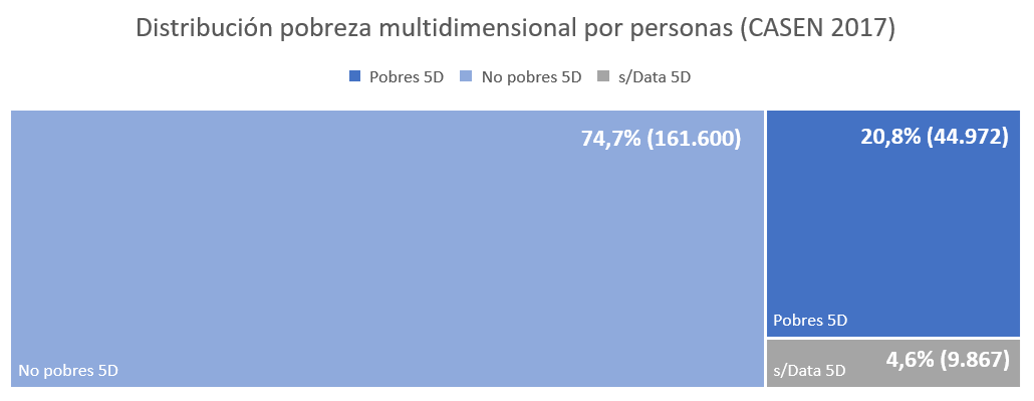
\includegraphics[width=\textwidth]{Mati N/pobrezaXpersonas.png}
    \caption{Distribución pobreza multidimensional por personas - CASEN 2017. Fuente: Elaboración propia.}
    \label{pobresXpersona}
\end{figure}

\begin{figure}[H]
    \centering
    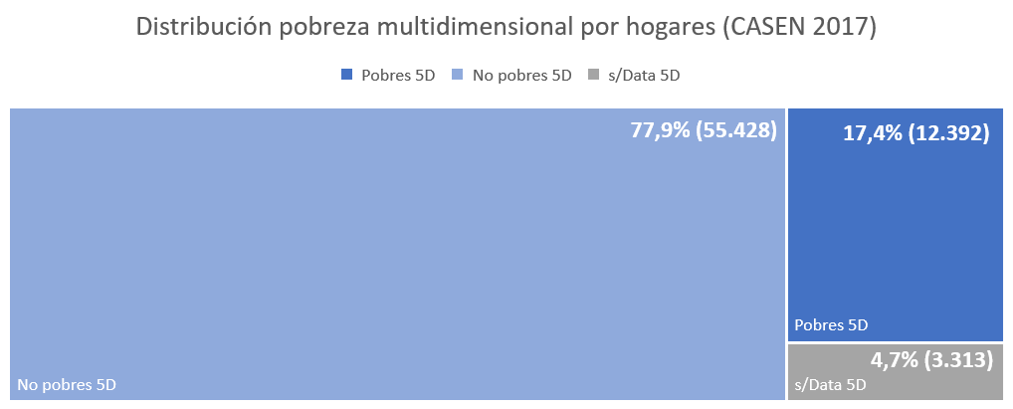
\includegraphics[width=\textwidth]{Mati N/pobrezaXhogares.png}
    \caption{Distribución pobreza multidimensional por hogares - CASEN 2017. Fuente: Elaboración propia.}
    \label{pobresXhogar}
\end{figure}
 

 
 Las variables de entrada para el modelo del análisis relacional corresponden, por lo tanto, al conjunto de indicadores de carencia para cada hogar pobre multidimensional, esto es, 12.392 indicadores de carencia por cada una de las 15 carencias. En la figura \ref{frecuenciatodos} se dispone de un resumen de la frecuencia de cada carencia en los hogares pobres multidimensionales. 


 \begin{figure}[H]
  \centering
    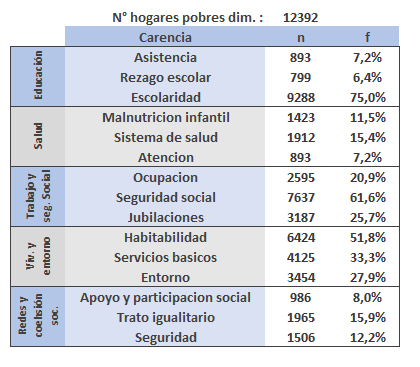
\includegraphics[height=9cm]{HOGARES/tabla_frec_general.png}
    \caption{Frecuencia de carencias hogares pobres multidimensionales. Fuente: Elaboración propia.}
    \label{frecuenciatodos}
\end{figure}
 

 
 Se puede apreciar que las 3 carencias más comunes (y también las únicas con una prevalencia superior al 50\%) corresponden a \textit{escolaridad} (75,0\%), \textit{seguridad social} (61,6\%) y \textit{habitabilidad} (51,8\%). En el otro extremo, las 4 carencias menos frecuentes (y que están presentes en menos del 10\% de los hogares pobres multidimensionales) son \textit{rezago escolar} (6,4\%), \textit{asistencia} (7,2\%), \textit{atención} (7,2\%) y \textit{apoyo y participación social} (8,0\%). 
 
 
 
 Para el cálculo de los coeficientes de correlación $\phi$ y $r$ (para los indicadores de carencias y los indicadores agregados dimensionales, respectivamente) se emplearon las bibliotecas de software libre NumPy y Pandas (Python).
 
 En la figura \ref{pearsoncarencias} se pueden observar los 105 resultados del cálculo del coeficiente $\phi$ entre los distintos pares de carencias, 35 de los cuales corresponden a valores positivos comprendidos en el intervalo [0,0018;0,0968], por lo que, en general, se puede decir que existe una relación de muy baja significancia entre las distintas carencias.
 


%%%%%%%%%%%%%%%%%%%% índice de pearson carencias
\begin{figure}[H]
    \centering
        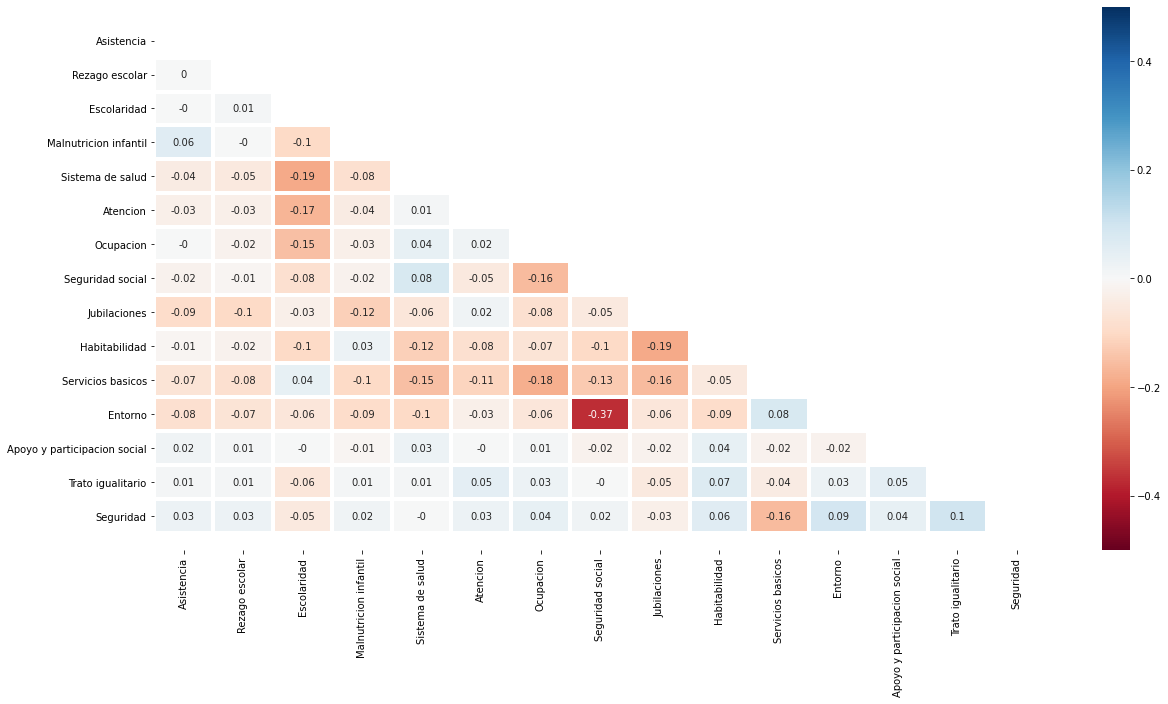
\includegraphics[width=\linewidth]{Heatmaps/Heatmap_pearson_Correlaciones.png}
    \caption{Mapa de calor coeficientes de correlación por carencias.Fuente: elaboración propia.}
    \label{pearsoncarencias}
\end{figure}



La red de carencias definida a partir de los resultados obtenidos en el cálculo de correlaciones se puede apreciar en la figura \ref{grafoPos}.

%%%%%%%%%%%%%%%%%%%% grafo carencias positivas
\begin{figure}[H]
    \centering
        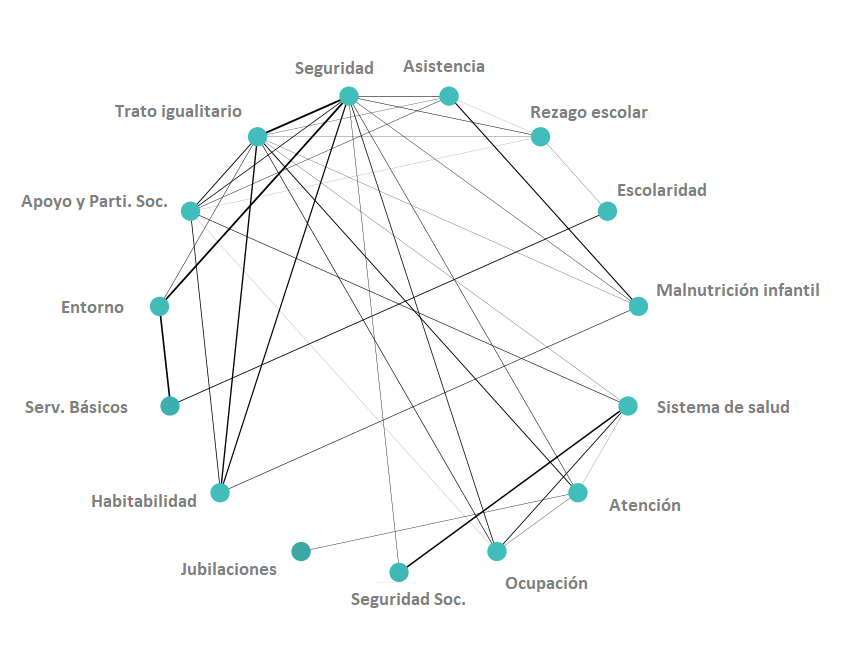
\includegraphics[width=11cm]{Grafos/GrafoCarencias.png}
    \caption{Red de carencias. Fuente: elaboración propia.}
    \label{grafoPos}
\end{figure}






%%%%%%%%%%%%%%%%%%%% analisis carencias positivas
\begin{figure}[H]
    \centering
        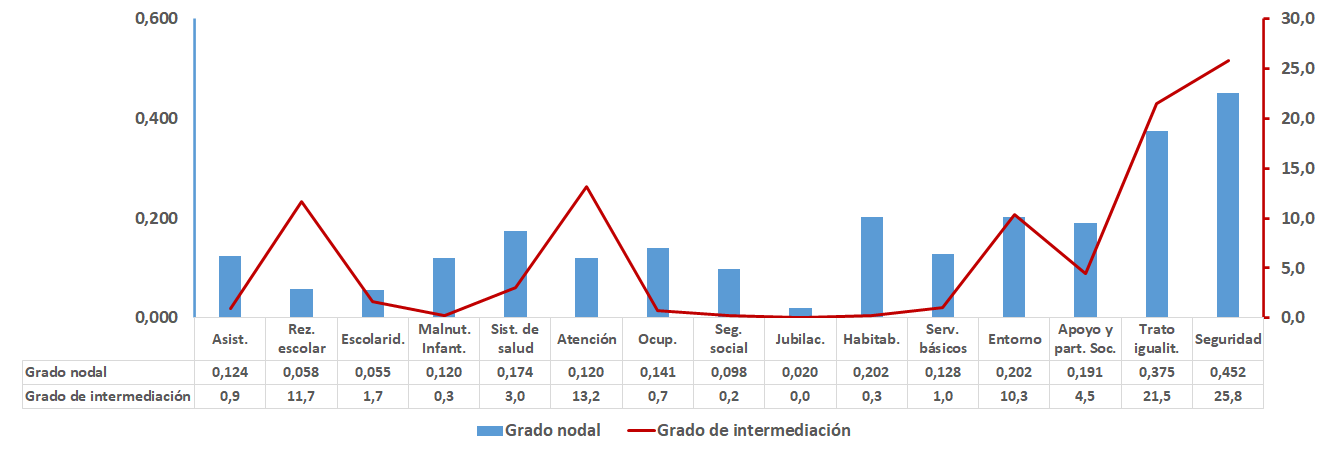
\includegraphics[width=\textwidth]{Grafos/nc_general.png}
    \caption{Medidas de centralidad de la red carencias. Fuente: elaboración propia.}
    \label{analisisPos}
\end{figure}

Observando las medidas de centralidad obtenidas de la red de carencias, se evidencia que las carencias con mayor grado nodal corresponden a \textit{seguridad} (0,452) y \textit{trato igualitario} (0,375), las que a su vez son las carencias con mayor grado de intermediación con 25,83 y 21,53 respectivamente. Es importante recordar que el grado nodal no tiene relación con las causas de la pobreza, sino que expresa, más bien, la importancia que tiene dicha carencia dentro de la red y que permite entender la dinámica interna de la pobreza. En este sentido, se podría decir que las carencias \textit{seguridad} y \textit{trato igualitario} serían buenos predictores simples de la pobreza multidimensional, y a su vez son aquellas que tienen en promedio una relación más significativa con el resto de las carencias. 


Los resultados del cálculo del coeficiente $r$ entre los indicadores dimensionales agregados (fig. \ref{PearsonDim}), muestran que, del total de 10 resultados, sólo 2 corresponden a relaciones positivas, comprendidas en el intervalo [0,0187;0,0435], lo cual indica una relación de muy baja significancia entre las carencias agregadas por dimensión.

%%%%%%%%%%%%%%%%%%%% índice de pearson DIM
\begin{figure}[H]
    \centering
        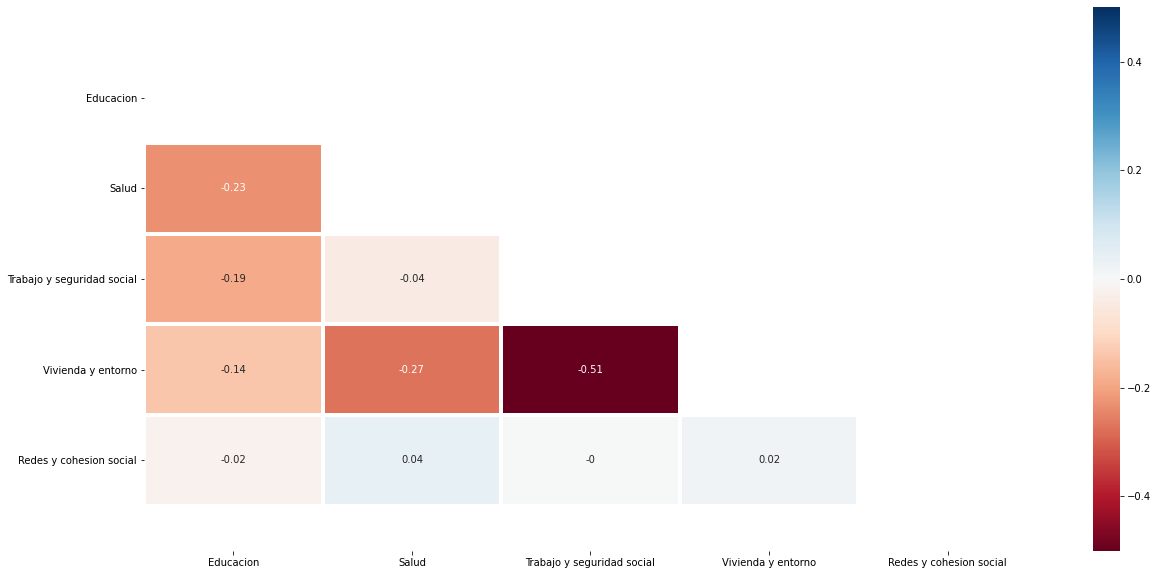
\includegraphics[width=\linewidth]{Heatmaps/Heatmap_pearson_DIM.png}
    \caption{Mapa de calor coeficientes de correlación por dimensiones. Elaboración propia}
    \label{PearsonDim}
\end{figure}

%%%%%%%%%%%%%%%%%%%%%%%%%%%%%% dimensiones
\begin{figure}[H]
  \centering
      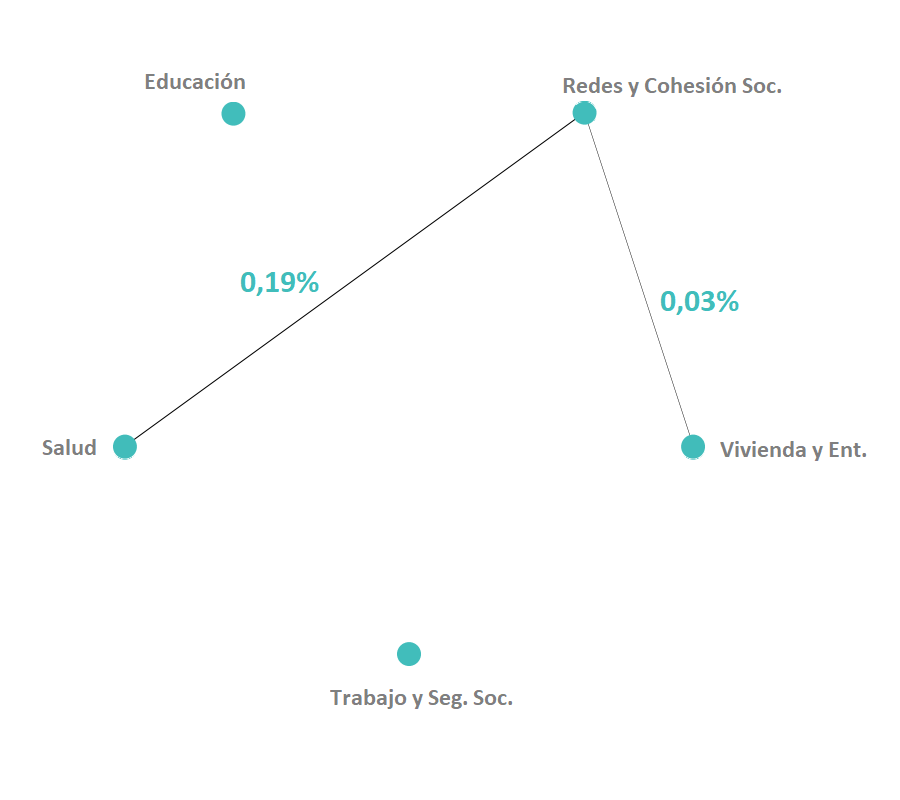
\includegraphics[height=9cm]{Grafos/GrafoDimensiones.png} 
    \caption{Red de dimensiones. Fuente: elaboración propia}
    \label{grafodimpos}
\end{figure}
%%%%%%%%%%%%%%%%%%%%%%%%%%%%%%%
%%%%%%%%%%%%%%%%%%%% analisis dim positivas
\begin{figure}[H]
    \centering
        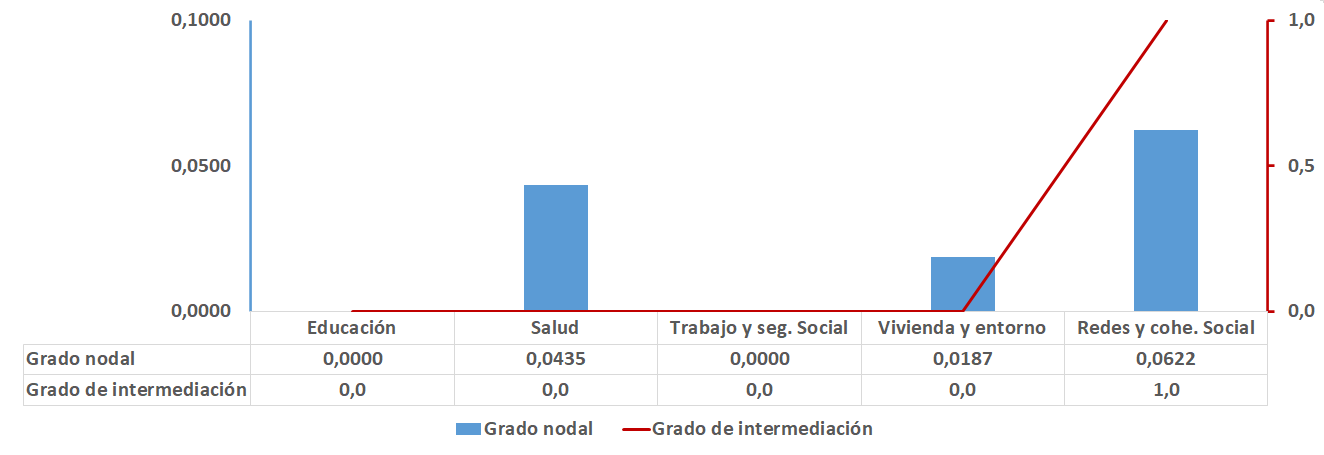
\includegraphics[width=\textwidth]{Grafos/nc_dimensional.png}
    \caption{Medidas de centralidad red de dimensiones. Elaboración propia.}
    \label{analisisDIMPOS}
\end{figure}




Las dimensiones con mayor grado nodal corresponden a \textit{Redes y cohesión social} (0,0622) y \textit{Salud} (0,0435), y la dimensión con mayor grado de intermediación corresponde a \textit{Redes y cohesión social} (1,00). Por lo tanto, la existencia de las carencias de las dimensiones  \textit{Redes y cohesión social} y \textit{Salud} tienden a estar más conectadas con el resto de las carencias de la red.



\subsection{Resultados análisis relacional por tipo de hogar y tipologías de la pobreza multidimensional}
%%%%%%%%%%%%%%%%%%%%%%%%%%%%%%%%%%%%%%%%%%%%%%%%%%%%%%%%%%%%%%%%%%%%%%%%%%%%%%%%%%%%%%%%%%%%% Resultados Mati N
En esta segunda etapa, a la muestra de hogares pobres multidimensionales se le aplicó la propiedad de descomponibilidad tomando en cuenta tres criterios (clasificación según tipo de hogar, zona de residencia y número de personas que componen el hogar), y se obtuvo, de este modo, distintos subconjuntos que permitieron focalizar el estudio. También se realizó un análisis comparativo entre la pobreza multidimensional y el nivel de ingresos de los hogares, empleando como medida de referencia la línea de la pobreza por ingresos LP.


\subsubsection{Análisis relacional por tipo de hogar}
La descomposición de la muestra por tipo de hogar generó 6 subgrupos de análisis, que corresponden a los 6 tipos de hogares según las definiciones especificadas en la metodología. En la figura \ref{distHogarTotal} se presenta la distribución de los hogares considerando la muestra total de hogares, y en la Figura \ref{distHogarpobres} se presenta la distribución de los hogares considerando la muestra de hogares pobres multidimensionales. 

\begin{figure}[H]
    \centering
    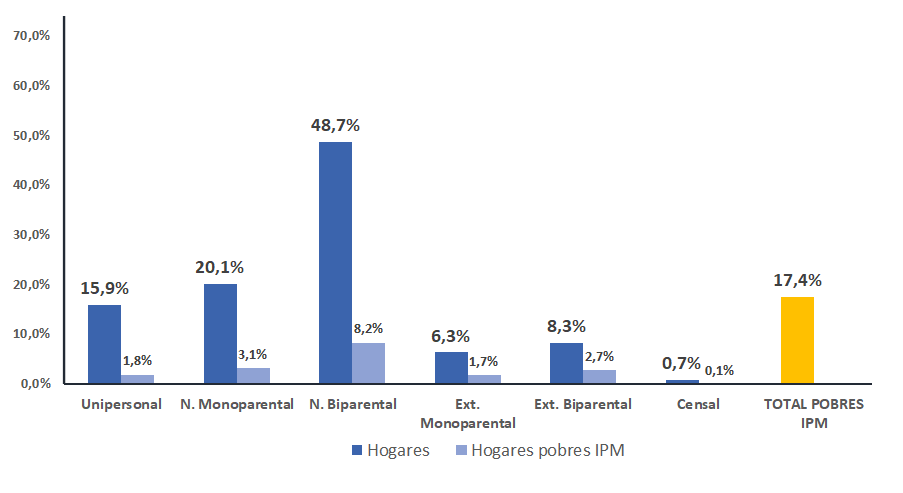
\includegraphics[width=\textwidth]{Max/distribucion_tipo_hogar_casen.png}
    \caption{Distribución por tipo de hogar. Fuente: elaboración propia.}
    \label{distHogarTotal}
\end{figure}

\begin{figure}[H]
    \centering
    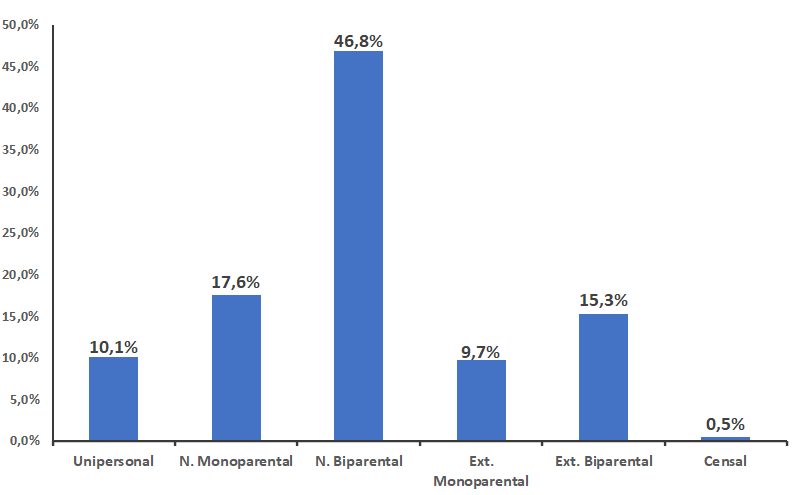
\includegraphics[width=\textwidth]{Max/distribucion_hog_pobres_por_tipo_hogar.png}
    \caption{Distribución por tipo de hogar, hogares pobres multidimensionales. Fuente: elaboración propia.}
    \label{distHogarpobres}
\end{figure}
Como se puede apreciar, el tipo de hogar biparental nuclear es el más presente en la muestra total y en la muestra de hogares pobres multidimensionales. Mientras que el tipo de hogar censal es el menos presente en la muestra total y en la muestra de hogares pobres multidimensionales. A continuación, se detallan los resultados para cada tipo de hogar.


\paragraph{Análisis relacional Hogar Unipersonal}

El subgrupo de hogares unipersonales está compuesto por 1.246 hogares pobres multidimensionales, los que representan el 10,1\% del total de hogares pobres multidimensionales. En la Figura \ref{freHUni} se presenta un resumen de la distribución de carencias de la muestra.
\begin{figure}[H]
    \centering
        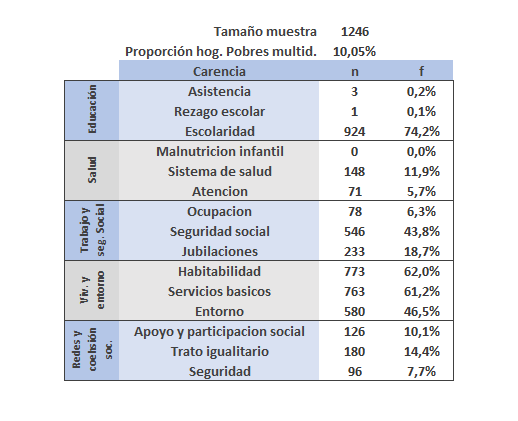
\includegraphics[height=9cm]{HOGARES/tabla_unip.png}
    \caption{Frecuencia de carencias Hogar Unipersonal. Fuente: Elaboración propia.}
    \label{freHUni}
\end{figure}
Como se puede observar, Escolaridad es la carencia más presente en los hogares unipersonales con una frecuencia de 74,2\%. Habitabilidad, Servicios básicos y Entorno, todas pertenecientes a la dimensión Vivienda y entorno, son las otras carencias más frecuentes. La carencia Malnutrición infantil no se encuentra presente en ningún hogar, y las carencias Asistencia Escolar y Rezago Escolar son las carencias menos presentes en los hogares, con frecuencias de 0,2\% y 0,1\% respectivamente. Esto resulta previsible debido a la definición de este tipo de hogar (hogares conformados por un solo integrante), ya que se espera que las personas que viven solas sean adultas. 

En la figura \ref{HMUni} se presenta el mapa de calor con las correlaciones entre las carencias y en la figura \ref{RedUnipos} la red de carencias.

\begin{figure}[H]
    \centering
        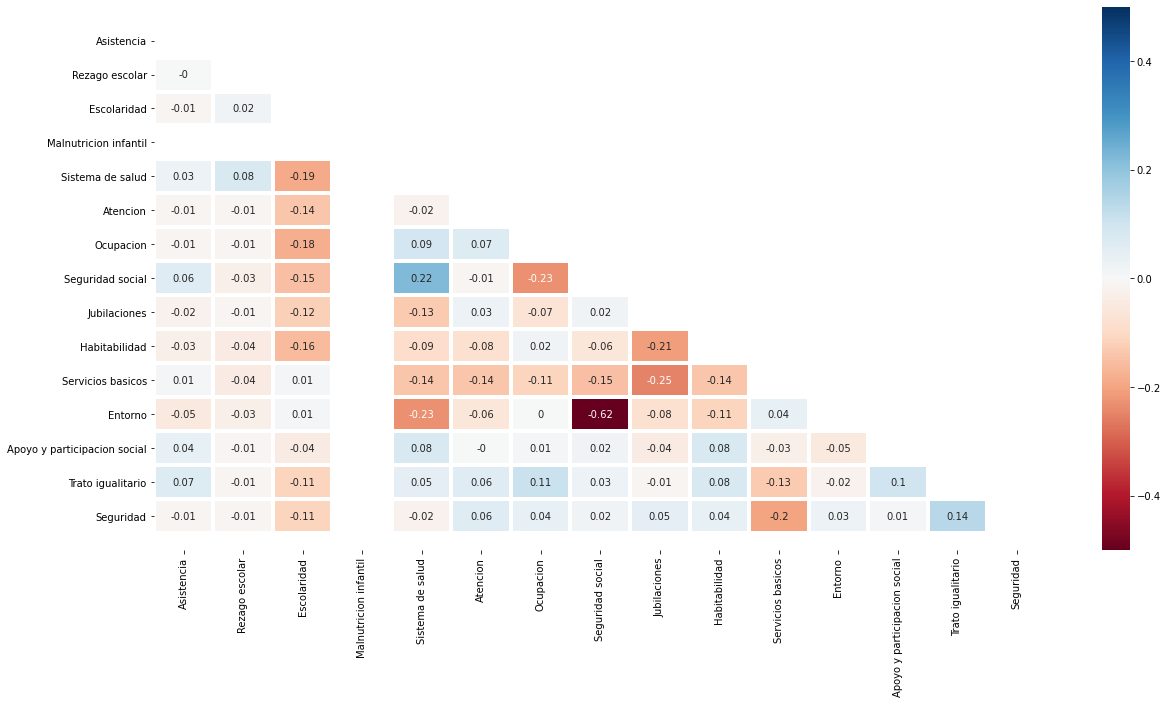
\includegraphics[height=10cm]{Heatmaps/Heatmap_pearson_car_unip.png}
    \caption{Coeficiente de correlación phi entre carencias Hogar unipersonal. Fuente: Elaboración propia.}
    \label{HMUni}
\end{figure}
\begin{figure}[H]
  \centering
    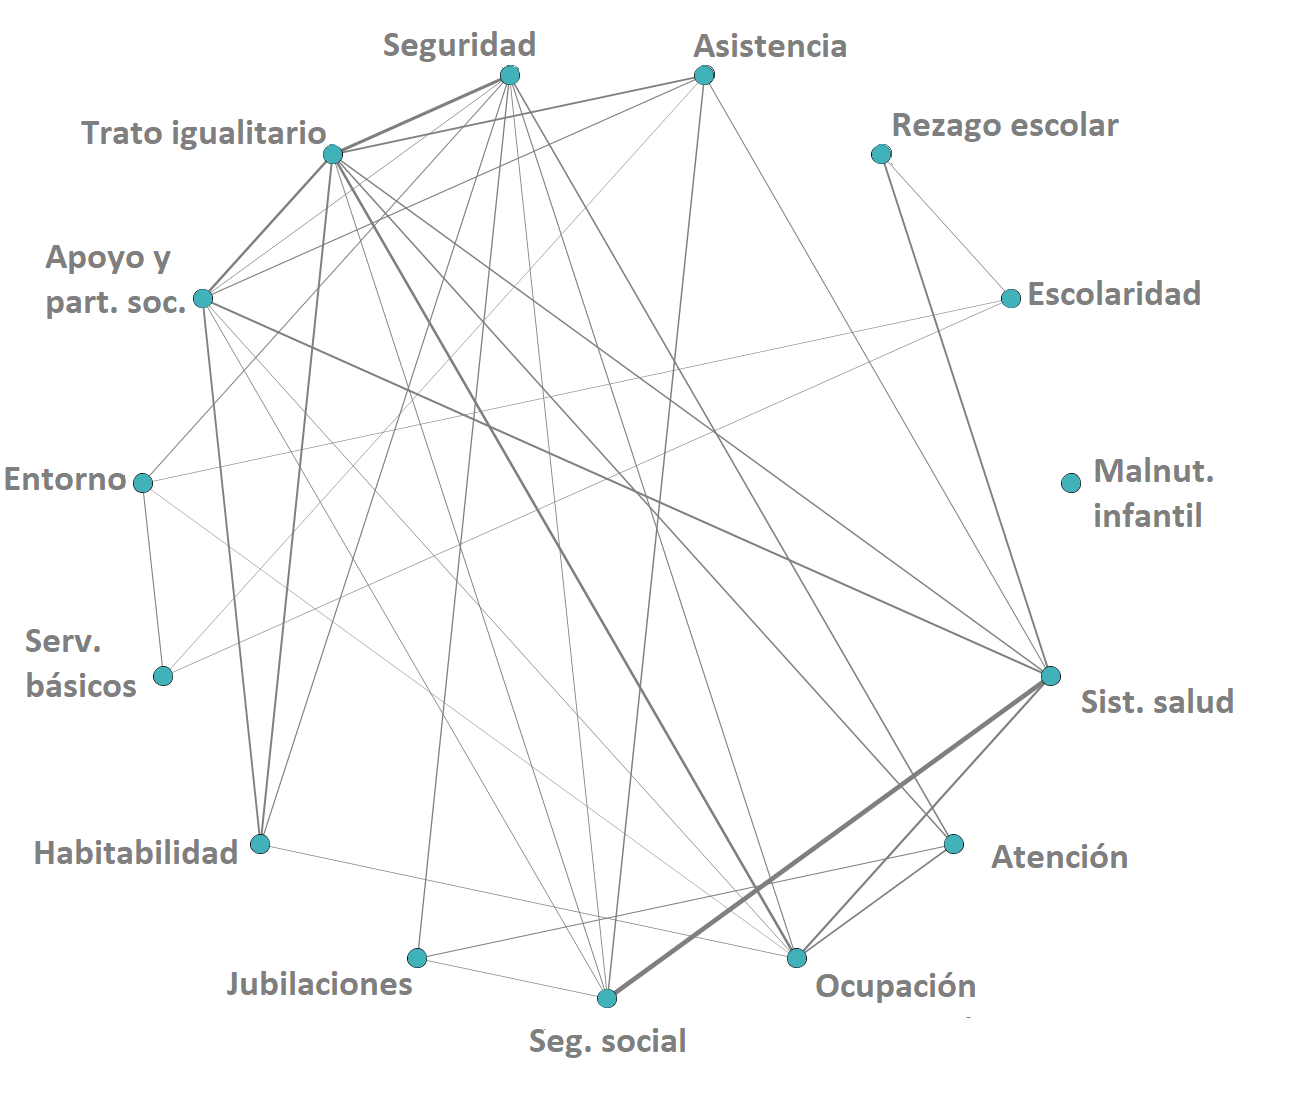
\includegraphics[height=8cm]{Grafos/grafo_unipersonal_pos.png}
    \caption{Red de carencias Hogar Unipersonal. Fuente: Elaboración propia.}
    \label{RedUnipos}
\end{figure}

En el mapa de calor y en las redes de correlaciones se puede observar que las correlaciones positivas más fuertes se presentan entre las carencias Seguridad social y Adscripción a sistema de salud (0,22), Trato igualitario y Seguridad (0,14), Trato igualitario y Ocupación (0,11), y Trato igualitario y Apoyo y participación social (0,1). 

En la figura \ref{CenUni} se muestran los pesos nodales y los grados de intermediación de la red de carencias.
\begin{figure}[H]
    \centering
    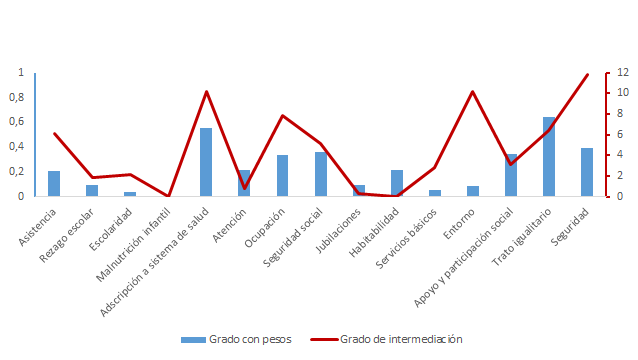
\includegraphics[width=\textwidth]{Grafos/nc_unipersonal.png}
    \caption{Medidas de centralidad Red de carencias Hogar Unipersonal. Fuente: elaboración propia.}
    \label{CenUni}
\end{figure}
Como se puede apreciar, las carencias con mayor grado nodal son Trato igualitario y Adscripción a sistema de salud, y las carencias con mayor grado de intermediación son Seguridad, Adscripción a sistema de salud y Entorno. 

Si bien Escolaridad es la carencia más presente en los hogares unipersonales, las dinámicas internas de este tipo de hogar sugieren que las carencias Adscripción a sistema de salud, Trato igualitario, Seguridad y Entorno podrían ser predictores simples de que un hogar es pobre multidimensional, debido a los vínculos que generan estas carencias con otras de la red. 

\paragraph{Análisis relacional Hogar Nuclear Monoparental }



El subgrupo de hogares nucleares monoparentales está compuesto por 2.180 hogares pobres multidimensionales, los que representan el 17,6\% del total de hogares pobres multidimensionales. En la figura \ref{freHMononuc} se muestran las distribuciones de las carencias.
\begin{figure}[H]
  \centering
    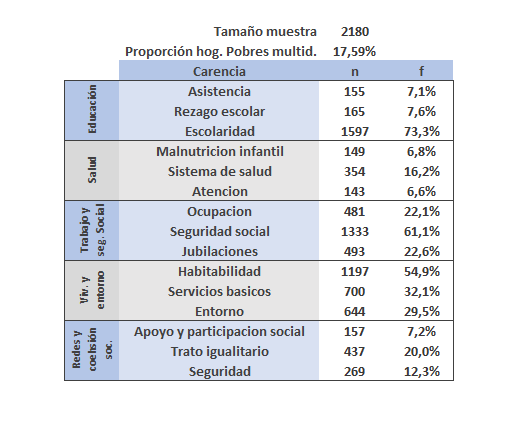
\includegraphics[height=9cm]{HOGARES/tabla_mononuc.png}
    \caption{Frecuencia carencias Hogar Nuclear Monoparental. Fuente: elaboración propia.}
    \label{freHMononuc}
\end{figure}
Como se puede observar, las carencias más frecuentes en este subgrupo son Escolaridad, Seguridad social y Habitabilidad con frecuencias de 73,3\%, 61,1\% y 54,9\% respectivamente. Mientras que las carencias menos frecuentes son Atención, Malnutrición infantil, Asistencia escolar, Apoyo y participación social y Rezago escolar.

En la figura \ref{HM_HMononuc} se presenta el mapa de calor con las correlaciones entre las distintas carencias, y en la figura \ref{RedMononucpos} la red de carencias.

\begin{figure}[H]
    \centering
    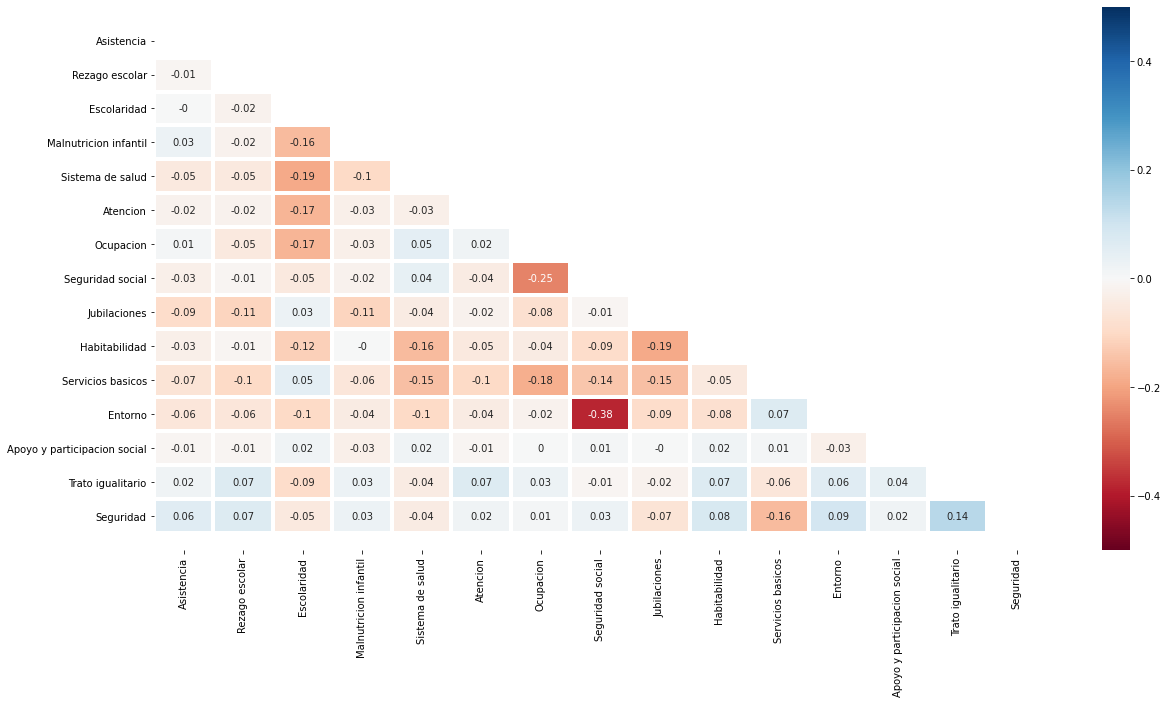
\includegraphics[height=10cm]{Heatmaps/Heatmap_pearson_car_monuc.png}
    \caption{Coeficiente de correlación phi entre carencias Hogar Nuclear Monoparental. Fuente: elaboración propia.}
    \label{HM_HMononuc}
\end{figure}

\begin{figure}[H]
  \centering

    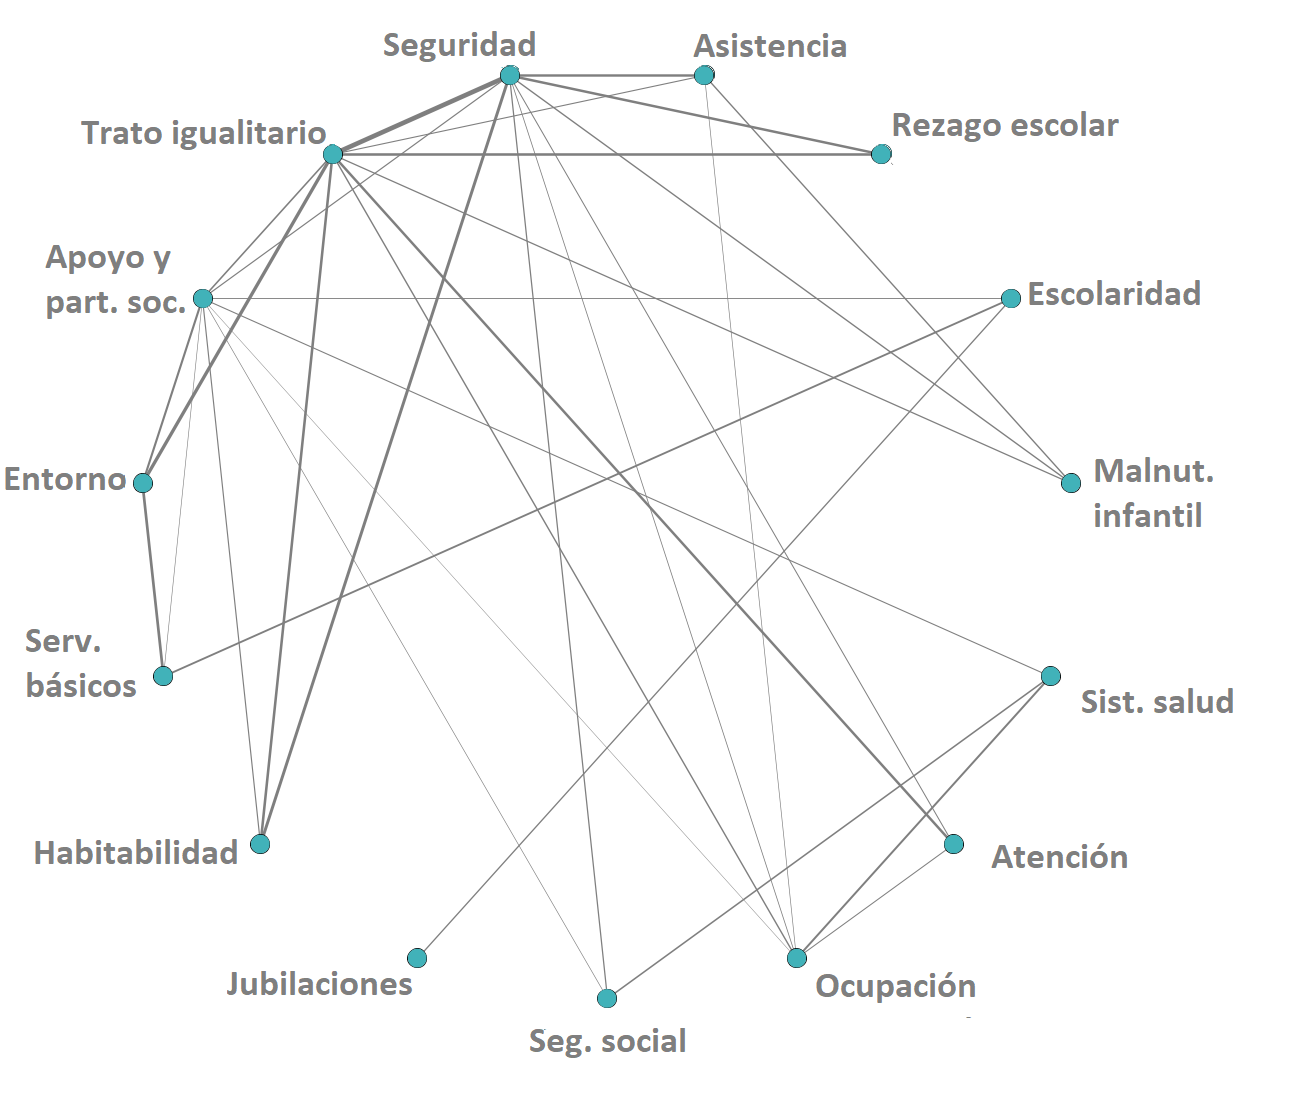
\includegraphics[width=10cm]{Grafos/grafo_mononuc_pos.png}
    \caption{Red de carencias Hogar Nuclear Monoparental. Fuente: elaboración propia.}
    \label{RedMononucpos}

\end{figure}

Las correlaciones positivas más fuertes se presentan entre las carencias Seguridad y Trato igualitario (0,14), Seguridad y Entorno (0,09), y Seguridad y Habitabilidad (0,08). 

\begin{figure}[H]
    \centering
    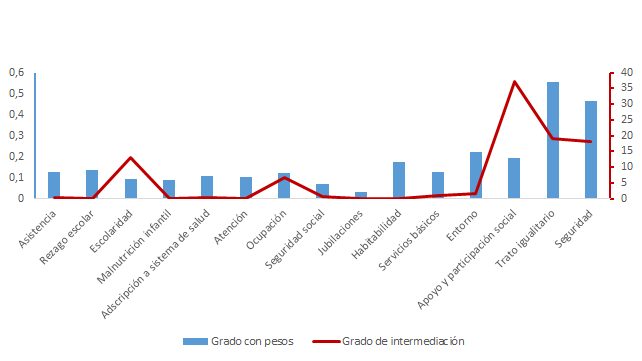
\includegraphics[width=\textwidth]{Grafos/nc_mononuc.png}
    \caption{Medidas de centralidad Red de carencias Hogar Monoparental Nuclear. Fuente: Elaboración propia.}
    \label{CenMononuc}
\end{figure}
Las carencias con mayor grado nodal son Trato igualitario (0,55) y Seguridad (0,46), y las carencias con mayor grado de intermediación son Apoyo y participación social (37,06), Trato igualitario (19,06), y Seguridad (18,1).

Las carencias Apoyo y participación social, Trato igualitario y Seguridad, pertenecientes a la dimensión Redes y cohesión social, son las que están más conectadas con el resto de las carencias de la red, y su manifestación en este tipo de hogar se considera un predictor simple para determinar que un hogar es pobre multidimensional.  

\paragraph{Análisis relacional Hogar Nuclear Biparental}
El subgrupo de hogares nucleares biparentales tiene un tamaño de muestra de 5.804 hogares pobres multidimensionales, que representan el 46,8\% del total de hogares pobres multidimensionales. En la Figura \ref{freBinuc} se presentan las distribuciones de las carencias.
\begin{figure}[H]
  \centering
    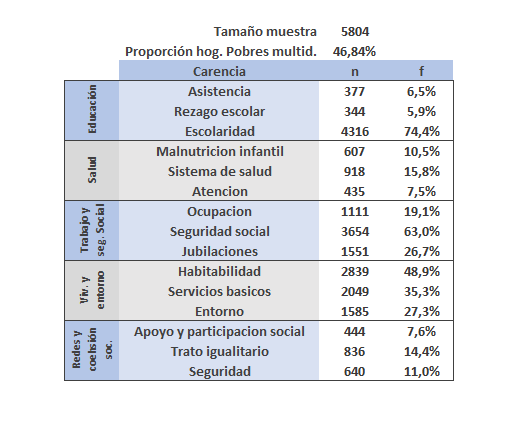
\includegraphics[height=9cm]{HOGARES/tabla_binuc.png}
    \caption{Frecuencia de carencias Hogar Nuclear Biparental. Fuente: elaboración propia.}
    \label{freBinuc}
\end{figure}
Las carencias más frecuentes son Escolaridad, Seguridad social y Habitabilidad con frecuencias de 74,4\%, 63\% y 48,9\% respectivamente. Mientras que las carencias menos frecuentes son Rezago escolar, Asistencia escolar, Atención de salud y Apoyo y participación social con frecuencias de 5,9\%, 6,5\% y 7,5\% respectivamente.

En la Figura \ref{HMBinuc} se presentan las correlaciones entre carencias y en la figura \ref{RedBinucpos} la red de carencias.
\begin{figure}[H]
    \centering
    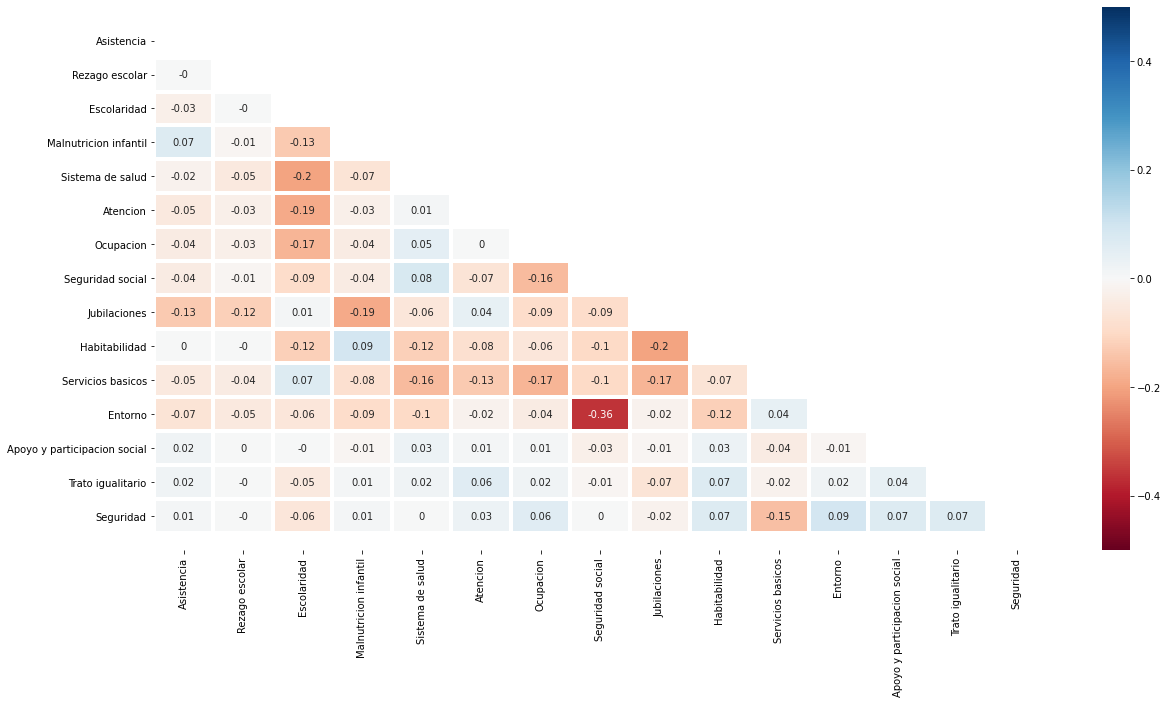
\includegraphics[height=10cm]{Heatmaps/Heatmap_pearson_car_binuc.png}
    \caption{Coeficiente de correlación phi entre carencias Hogar Nuclear Biparental. Fuente: elaboración propia.}
    \label{HMBinuc}
\end{figure}

\begin{figure}[H]
  \centering
    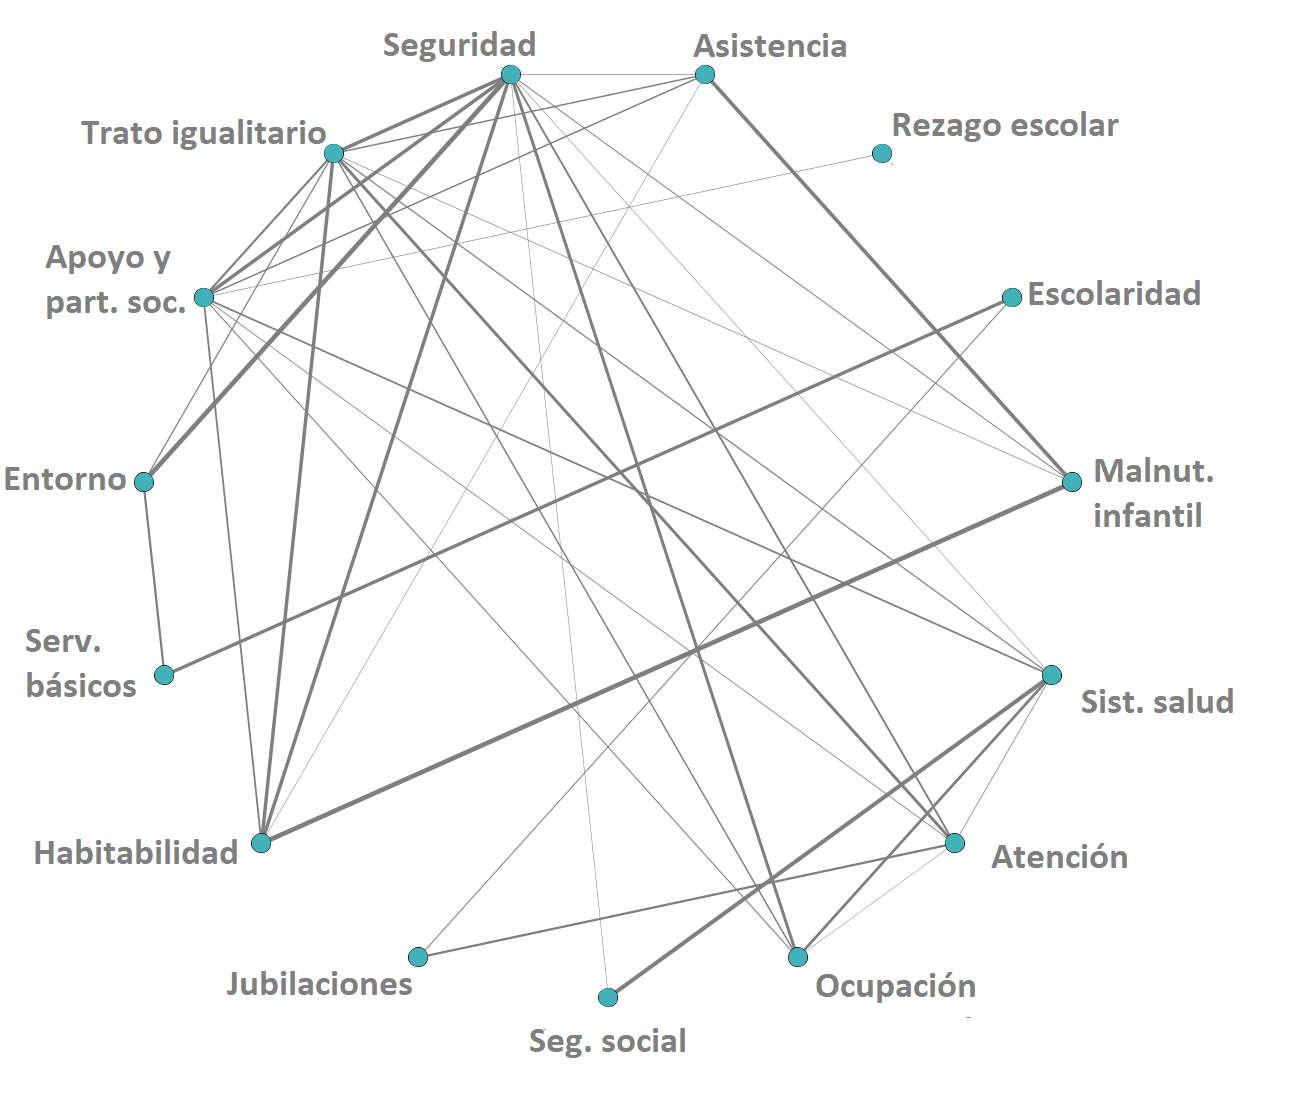
\includegraphics[width=10cm]{Grafos/grafo_binuc_pos.png}
    \caption{Red de carencias Hogar Nuclear Biparental. Fuente: elaboración propia.}
    \label{RedBinucpos}
\end{figure}

Las correlaciones positivas más fuertes se presentan entre las carencias Habitabilidad y Malnutrición infantil (0,09), Seguridad y Entorno (0,09), y Seguridad social y Sistema de salud (0,08). 

En la figura \ref{CenBinuc} se muestran los grados nodales y los grados de intermediación de la red de carencias. 
\begin{figure}[H]
    \centering
    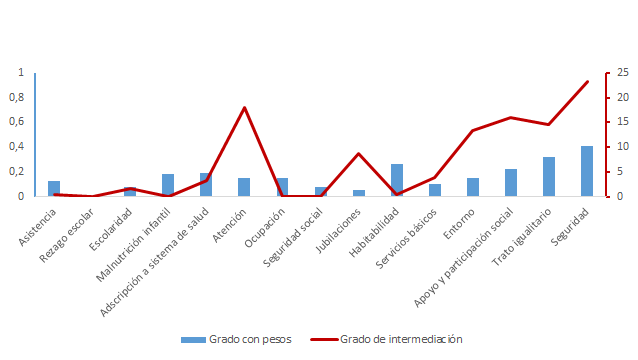
\includegraphics[width=\textwidth]{Grafos/nc_binuc.png}
    \caption{Medidas de centralidad Red de carencias Hogar Nuclear Biparental. Fuente: elaboración propia.}
    \label{CenBinuc}
\end{figure}
Las carencias con mayor grado nodal son Seguridad (0,41) y Trato igualitario (0,32). Mientras que las carencias con mayor grado de intermediación son Seguridad (23,3), Atención de salud (18,03), Apoyo y participación social (16,06) y Trato igualitario (14,63).

Las carencias Apoyo y participación social, Trato igualitario y Seguridad, pertenecientes a la dimensión Redes y cohesión social, y Atención de salud, son las que están más conectadas con otras carencias, lo que permite que actúen como predictores simples en este tipo de hogar para identificar a un hogar pobre multidimensional.  

\paragraph{Análisis relacional Hogar Extendido Monoparental}

El subgrupo de hogares extendidos monoparentales comprende 1.202 hogares, que representan el 9,7\% del total de hogares pobres multidimensionales. En la Figura \ref{freMonoex} se muestran las distribuciones de las carencias.

\begin{figure}[H]
  \centering
    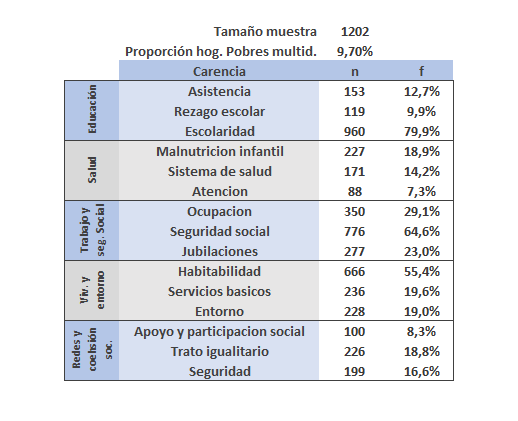
\includegraphics[height=9cm]{HOGARES/tabla_monoex.png}
    \caption{Frecuencia de carencias Hogar Extendido Monoparental. Fuente: elaboración propia.}
    \label{freMonoex}
\end{figure}
Como se puede observar, las carencias más frecuentes son Escolaridad, Seguridad social y Habitabilidad, con frecuencias de 79,9\%, 64,6\% y 55,4\% respectivamente. Las carencias menos frecuentes son Atención de salud, Apoyo y participación social, y Rezago escolar.

En la Figura \ref{HMMonoex} se presenta el mapa de calor de las correlaciones entre carencias y en la figura \ref{RedMonoexpos} la red de carencias.

\begin{figure}[H]
    \centering
    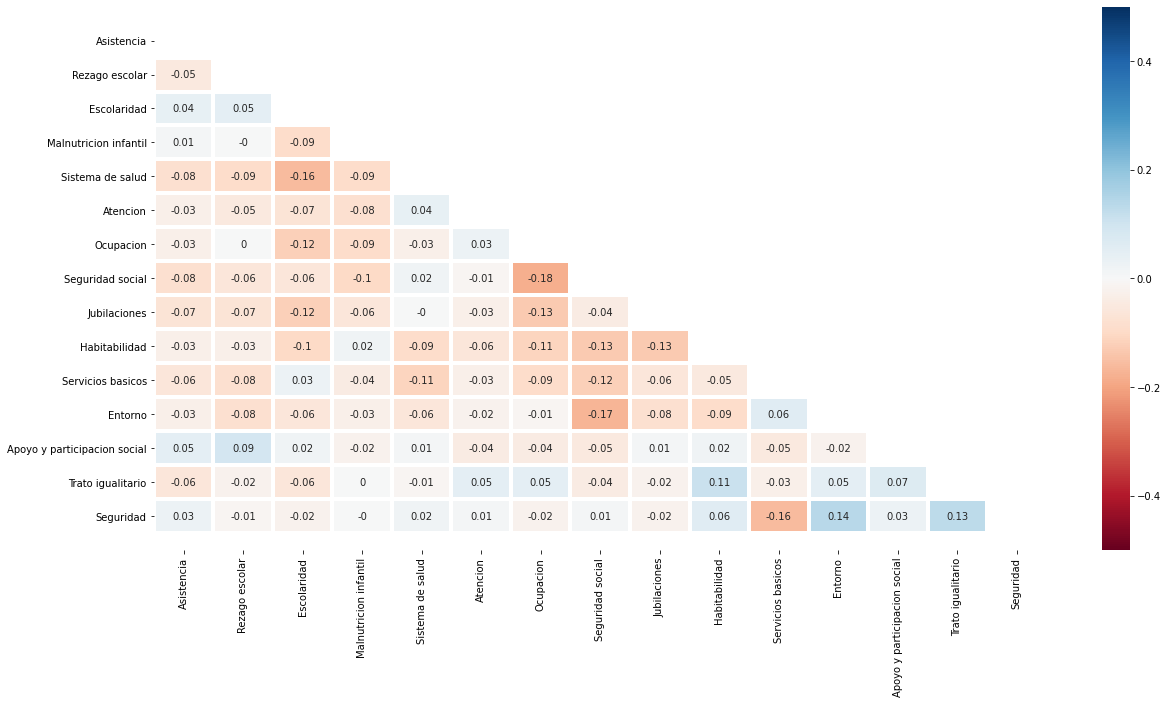
\includegraphics[height=10cm]{Heatmaps/Heatmap_pearson_car_monoex.png}
    \caption{Coeficiente de correlación phi entre carencias Hogar Extendido Monoparental. Fuente: elaboración propia.}
    \label{HMMonoex}
\end{figure}

\begin{figure}[H]
  \centering
    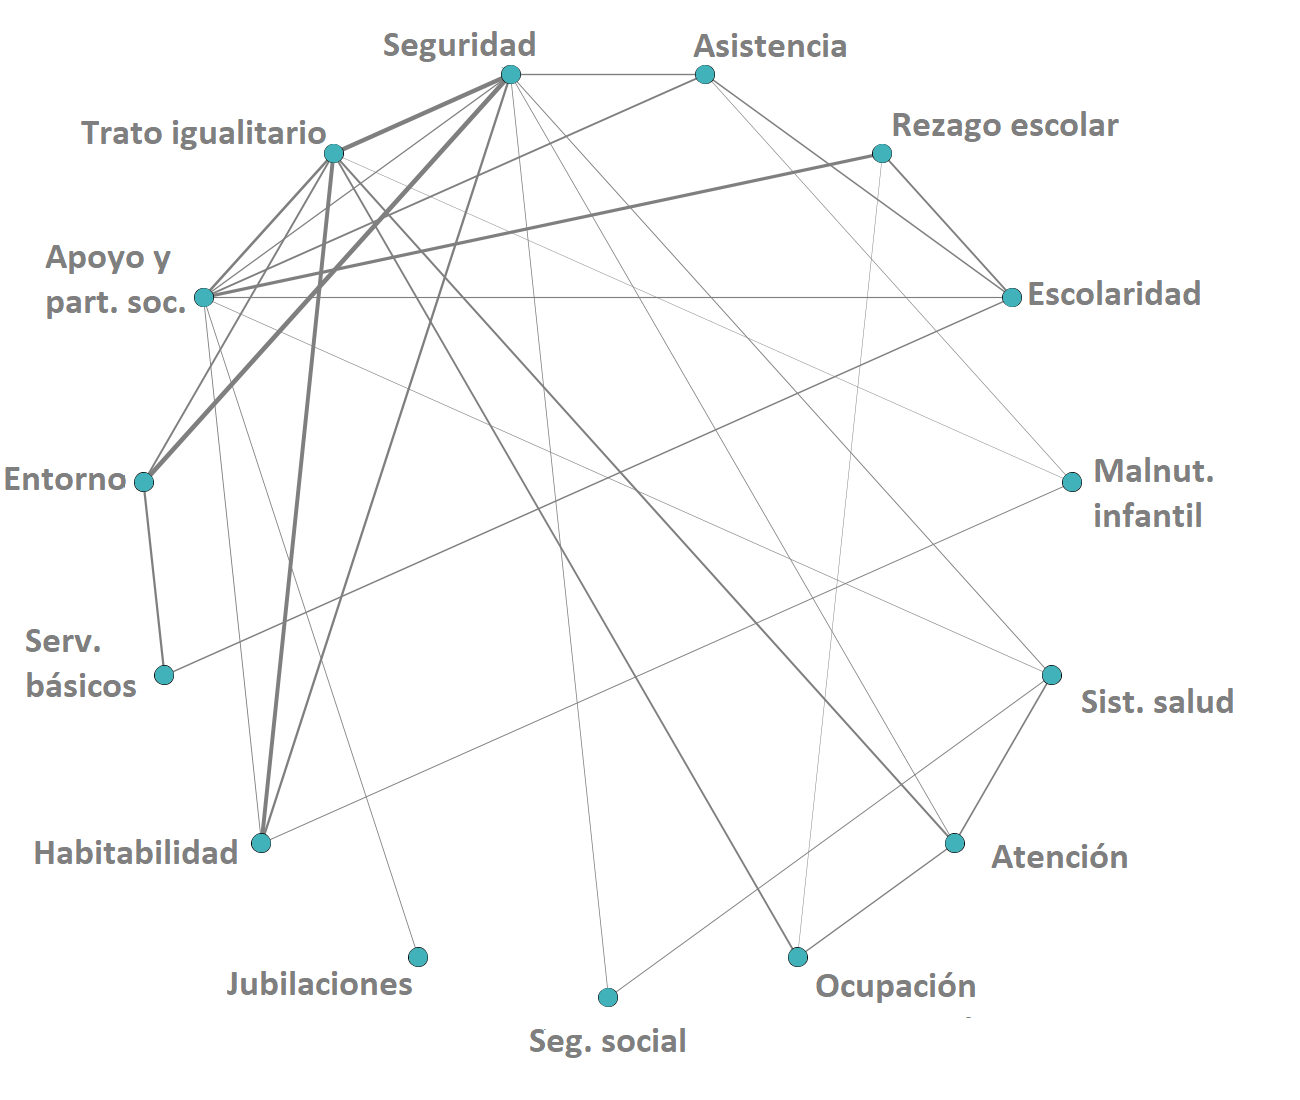
\includegraphics[width=10cm]{Grafos/grafo_monoex_pos.png}
    \caption{Red de carencias Hogar Extendido Monoparental. Fuente: elaboración propia.}
    \label{RedMonoexpos}
\end{figure}
Las correlaciones positivas más fuertes se presentan entre las carencias Seguridad y Entorno (0,14), Seguridad y Trato igualitario (0,13) y Trato igualitario y Habitabilidad (0,11). 

En la figura \ref{CenMonoex} se muestran los grados nodales y grados de intermediación de la red de carencias.

\begin{figure}[H]
    \centering
    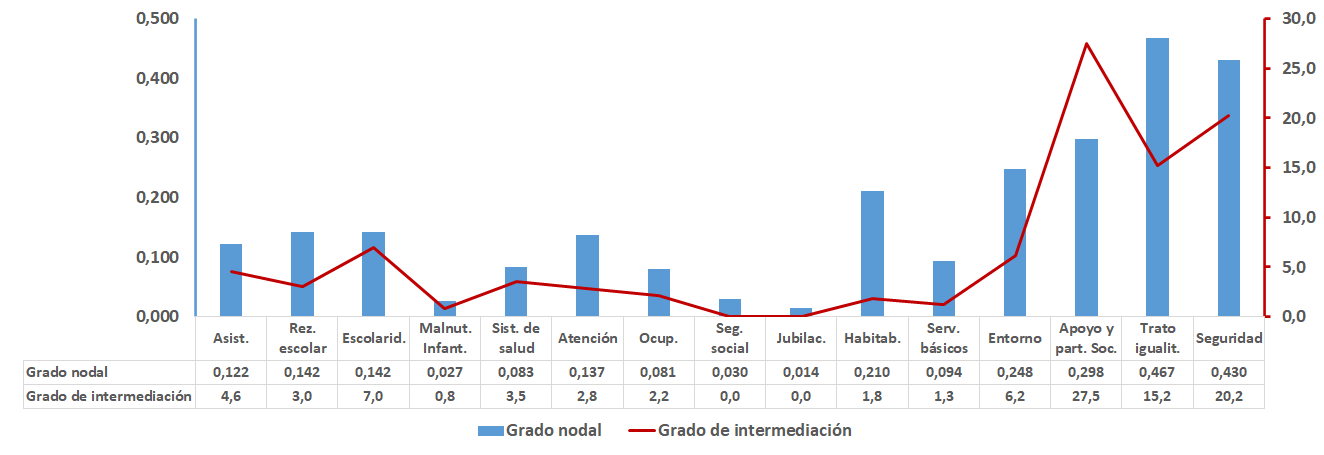
\includegraphics[width=\textwidth]{Grafos/nc_monoex.png}
    \caption{Medidas de centralidad Red de carencias Hogar Extendido Monoparental. Fuente: elaboración propia.}
    \label{CenMonoex}
\end{figure}
Las carencias con mayor grado nodal son Trato igualitario (0,46) y Seguridad (0,43) y las carencias con mayor grado de intermediación son Apoyo y participación social (27,46), Seguridad (20,24) y Trato igualitario (15,19).

Las carencias Apoyo y participación social, Trato igualitario y Seguridad, pertenecientes a la dimensión Redes y cohesión social, son las que presentan más conexiones con el resto de las carencias de la red, por lo que su manifestación en este tipo de hogar podría considerarse un predictor simple de que el hogar es pobre multidimensional.


\paragraph{Análisis relacional Hogar Extendido Biparental}

El subgrupo de hogares extendidos biparentales tiene un tamaño de 1.894 hogares, que representan el 15,3\% de los hogares pobres multidimensionales. En la figura \ref{freBiex} se muestran las distribuciones de las carencias.

\begin{figure}[H]
  \centering
    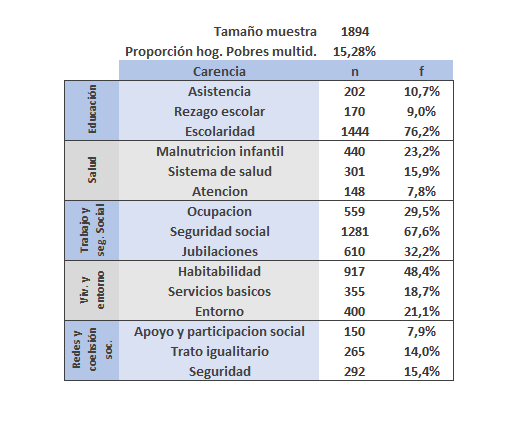
\includegraphics[height=9cm]{HOGARES/tabla_biex.png}
    \caption{Frecuencia de carencias Hogar Extendido Biparental. Fuente: elaboración propia.}
    \label{freBiex}
\end{figure}

Como se puede apreciar, las carencias más frecuentes son Escolaridad (76,2\%), Seguridad social (67,6\%) y Habitabilidad (48,4\%). Las carencias menos frecuentes son Atención de salud (7,8\%), Apoyo y participación social (7,9\%) y Rezago escolar (9,0\%).

En la Figura \ref{HMBiex} se presenta un mapa de calor de las correlaciones entre carencias y en la figura \ref{RedBiexpos} la red de carencias.

\begin{figure}[H]
    \centering
    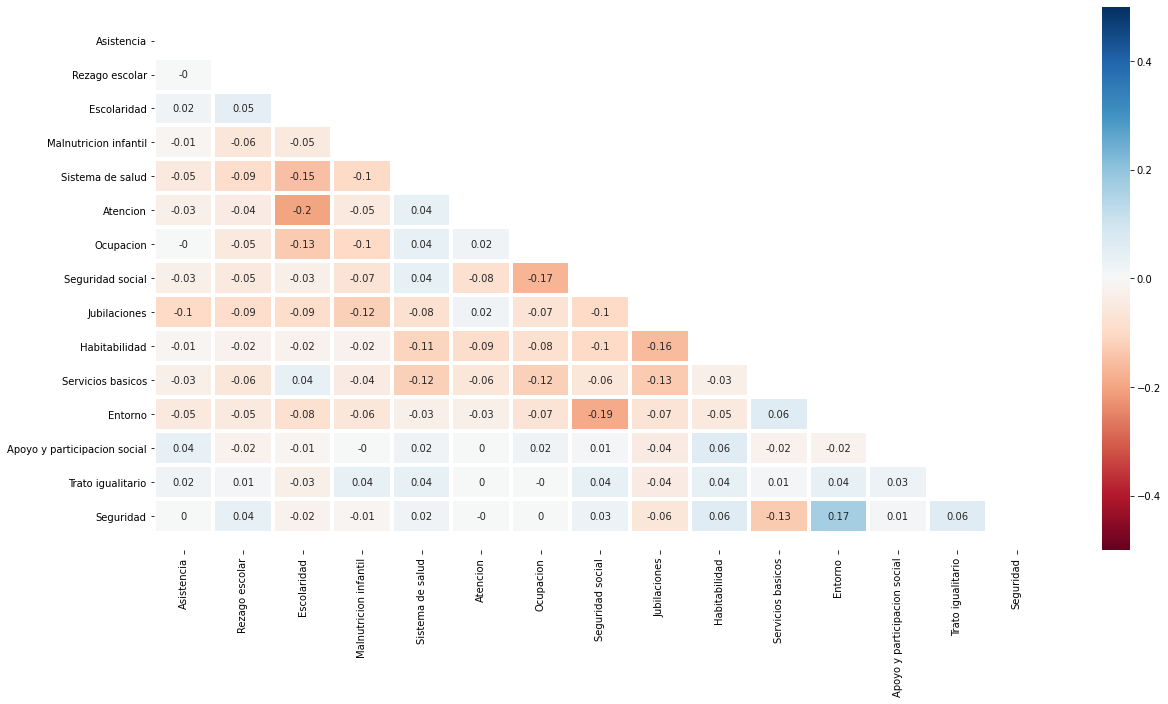
\includegraphics[width=\textwidth]{Heatmaps/Heatmap_pearson_car_biex.png}
    \caption{Coeficiente de correlación phi entre carencias Hogar Extendido Biparental. Fuente: elaboración propia.}
    \label{HMBiex}
\end{figure}

\begin{figure}[H]
  \centering
    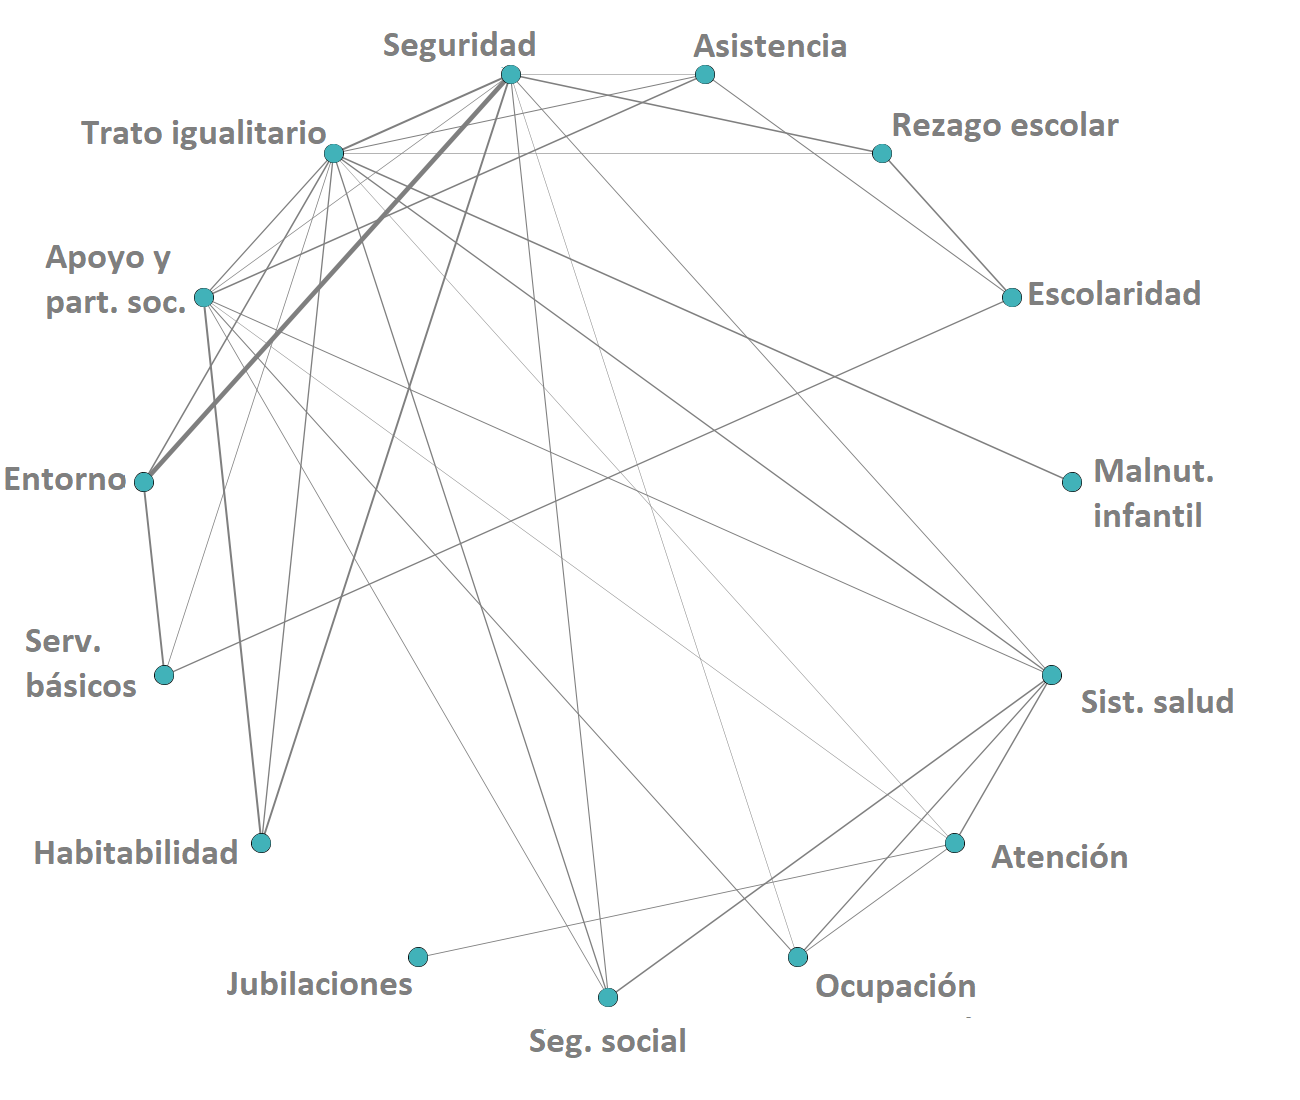
\includegraphics[width=10cm]{Grafos/grafo_biex_pos.png}
    \caption{Red de carencias Hogar Extendido Biparental. Fuente: elaboración propia.}
    \label{RedBiexpos}
\end{figure}

La correlación positiva más fuerte se presenta entre las carencias Seguridad y Entorno (0,17). 

En la Figura \ref{CenBiex} se muestran los grados nodales y grados de intermediación de la red de carencias.

\begin{figure}[H]
    \centering
    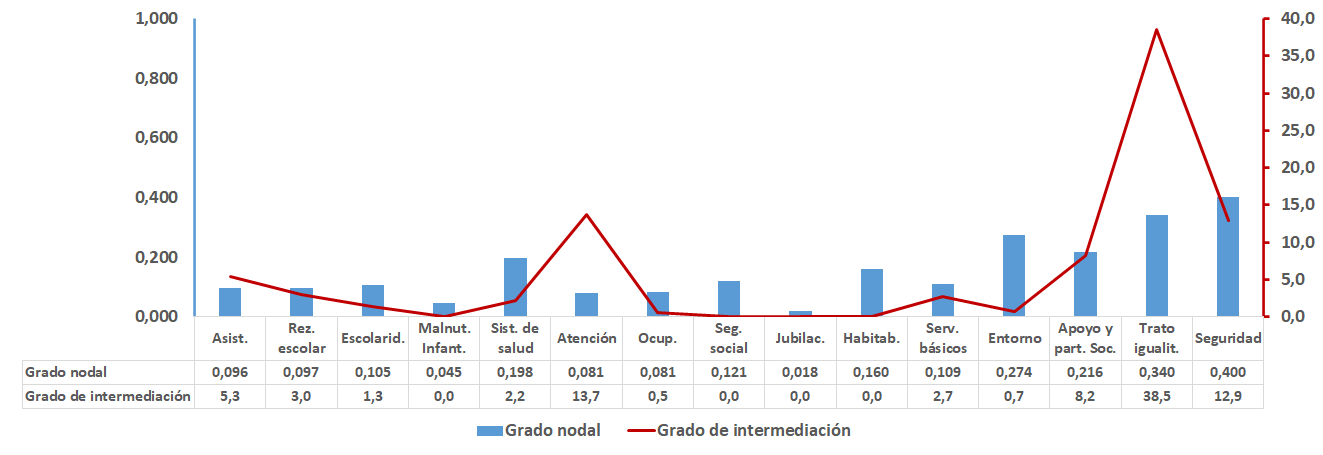
\includegraphics[width=\textwidth]{Grafos/nc_biex.png}
    \caption{Medidas de centralidad Red de Carencias Hogar Extendido Biparental. Fuente: elaboración propia.}
    \label{CenBiex}
\end{figure}
Las carencias con mayor grado nodal son Seguridad (0,40), Trato igualitario (0,34) y Entorno (0,27). Las carencias con mayor grado de intermediación son Trato igualitario (38,47), Atención de salud (13,7) y Seguridad (12,9).

Trato igualitario, Seguridad, Atención de salud y Entorno son las carencias más conectadas con el resto de las carencias de la red, por lo que su manifestación en este tipo de hogar podría considerarse un predictor simple de que dicho hogar es pobre multidimensional. 

\paragraph{Análisis relacional Hogar Censal}
El subgrupo de hogares censales comprende 66 hogares, que representan el 0,5\% del total de hogares pobres multidimensionales. En la figura \ref{freCensal} se presenta la distribución de carencias de la muestra.
\begin{figure}[H]
  \centering
    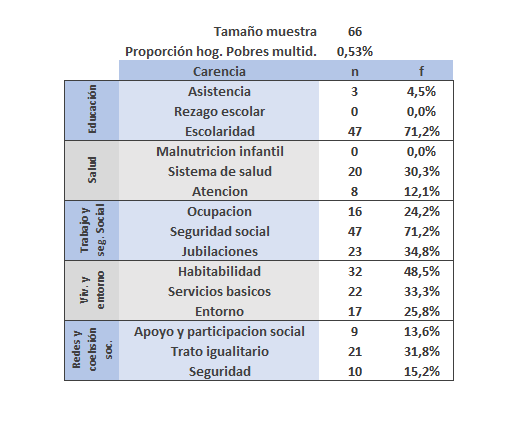
\includegraphics[height=9cm]{HOGARES/tabla_censal.png}
    \caption{Frecuencia de carencias Hogar Censal. Fuente: elaboración propia.}
    \label{freCensal}
\end{figure}
Como se puede apreciar, las carencias más frecuentes son Escolaridad y Seguridad social, ambas con frecuencias de 71,2\%. Las carencias Rezago escolar y Malnutrición infantil no se encuentran presentes en ningún hogar, y Asistencia escolar es la carencia menos frecuente, lo que resulta previsible considerando la definición de hogar censal, ya que se espera que los integrantes de este tipo de hogar no sean niños. 

En la figura \ref{HMCensal} se presenta el mapa de calor de las correlaciones entre carencias y en la figura \ref{RedCensalpos} la red de carencias.

\begin{figure}[H]
    \centering
    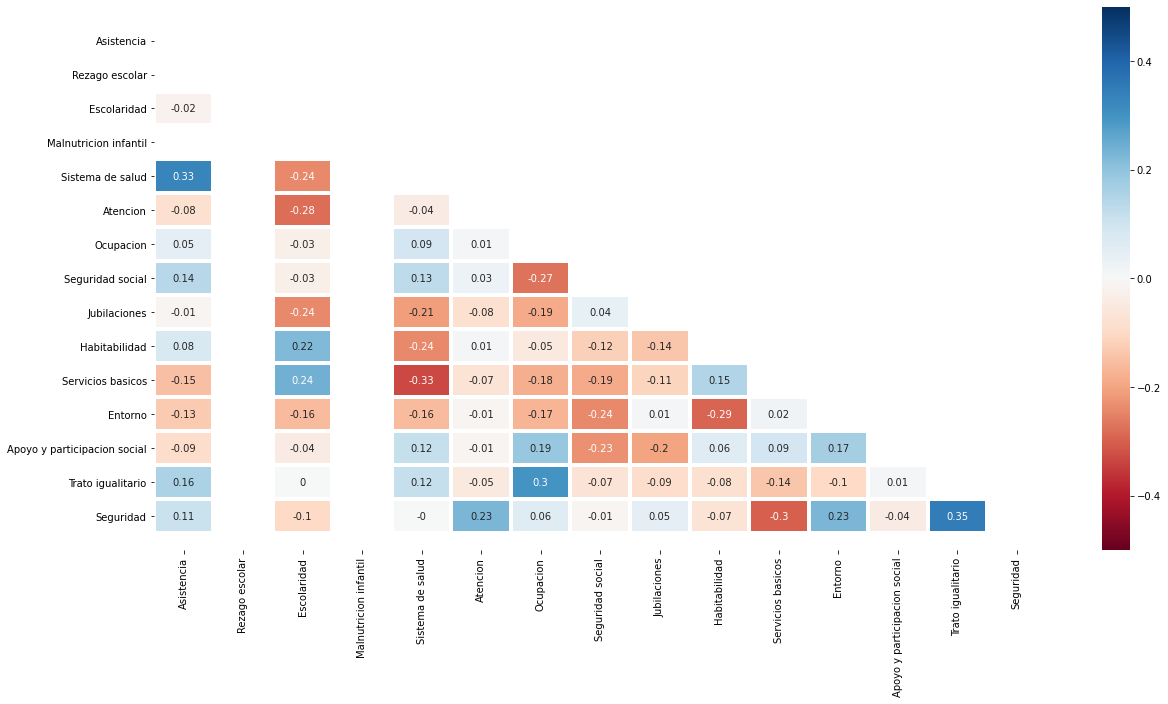
\includegraphics[width=\textwidth]{Heatmaps/Heatmap_pearson_car_censal.png}
    \caption{Coeficiente de correlación phi entre carencias Hogar Censal. Fuente: elaboración propia.}
    \label{HMCensal}
\end{figure}

\begin{figure}[H]
  \centering
    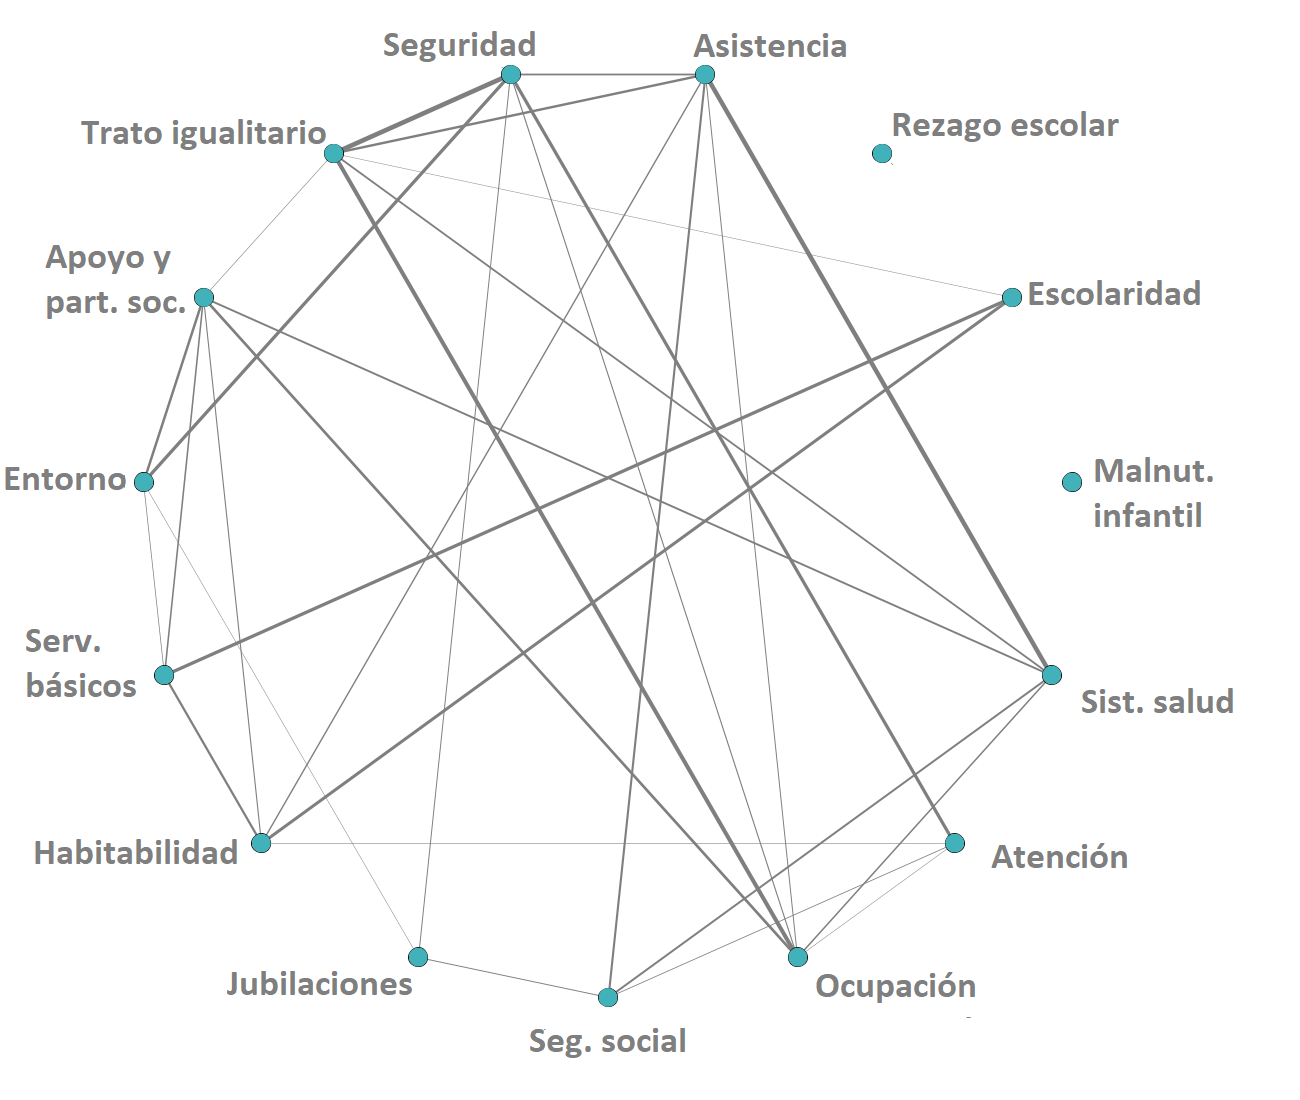
\includegraphics[width=10cm]{Grafos/grafo_censal_pos.png}
    \caption{Red de carencias Hogar Censal. Fuente: elaboración propia.}
    \label{RedCensalpos}
\end{figure}


Las correlaciones positivas más fuertes se presentan entre las carencias Seguridad y Trato igualitario (0,35), Sistema de salud y Asistencia escolar (0,33) y Ocupación y Trato igualitario (0,3). 

En la figura \ref{CenCensal} se muestra un gráfico con los grados nodales y grados de intermediación de la red de carencias.

\begin{figure}[H]
    \centering
    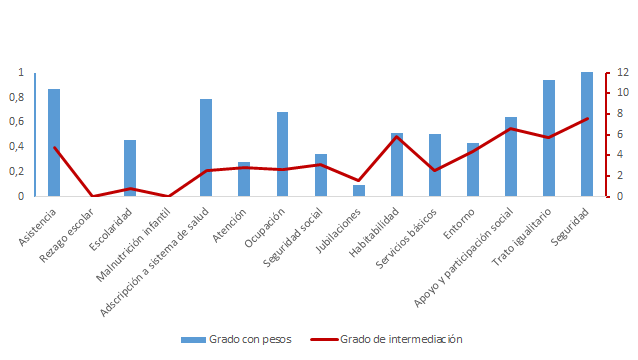
\includegraphics[width=\textwidth]{Grafos/nc_censal.png}
    \caption{Medidas de centralidad Red de carencias Hogar Censal. Fuente: elaboración propia.}
    \label{CenCensal}
\end{figure}
Las carencias con mayor grado nodal son Seguridad (1,03), Trato igualitario (0,94) y Asistencia escolar (0,87). Las carencias con mayor grado de intermediación son Seguridad (7,58) y Apoyo y participación social (6,58).

Las carencias Seguridad, Trato igualitario, Apoyo y participación social, y Asistencia escolar son las que presentan mayor cantidad de conexiones con el resto de las carencias de la red, por lo que su manifestación en este tipo de hogar podría considerarse un predictor simple de que el hogar es pobre multidimensional. 




\subsubsection{Análisis tipológico de la pobreza multidimensional}
Las tipologías de las carencias son combinaciones específicas de carencias que se manifiestan en los hogares. Su identificación permite conocer cómo la pobreza afecta a los hogares pobres multidimensionales a través de las privaciones. En la figura \ref{TipGen} se muestran las tipologías más frecuentes de la muestra original de hogares pobres multidimensionales.
\begin{figure}[H]
    \centering
    \includegraphics[width=\textwidth]{Mati N/tipologíaGeneral.png}
    \caption{Tipologías de carencias más frecuentes de los hogares pobres multidimensionales. Fuente: elaboración propia.}
    \label{TipGen}
\end{figure}
Como se puede observar, existen 1.849 tipologías de carencias en los hogares pobres multidimensionales, y las 10 más frecuentes representan el 24,59\% de los hogares. Dentro de los aspectos importantes que se desprenden de estas tipologías, destaca la incidencia que tiene Escolaridad, lo que se condice con las altas frecuencias que presenta en todos los tipos de hogares, y la ausencia de las carencias de la dimensión Redes y cohesión social, que en los análisis por tipo de hogar presentan las centralidades más importantes. Esto último refleja la diferencia que existe entre la aproximación estadística y relacional. También resulta importante notar que el 80\% de las tipologías presenta un \textit{IPM} de 22,5\%, lo que significa que los hogares son pobres multidimensionales en el margen, con la cantidad de carencias mínimas.

Luego de obtener las tipologías de los hogares pobres multidimensionales, se aplicó la propiedad de descomponibilidad tomando en cuenta el número de personas que habitan en un hogar y la zona de residencia, criterios que para efectos de este trabajo son considerados factores externos, ya que no afectan el cálculo del índice de pobreza multidimensional (\textit{IPM}).

\paragraph{Análisis tipológico por número de personas en el hogar}


La descomposición de la muestra de hogares pobres multidimensionales por número de personas en el hogar generó 7 subgrupos de análisis, los cuales fueron analizados considerando las tipologías y las frecuencias de las carencias. A continuación, se detallan los resultados para cada subgrupo.
\begin{itemize}
    \item \textbf{Hogares de 1 integrante}

    El subgrupo de hogares de 1 integrante es idéntico al subgrupo de hogares unipersonales. Reúne a 1.246 hogares que representan el 10,05\% de los hogares pobres multidimensionales. En las figuras \ref{fren1} y \ref{tipn1} se presentan las frecuencias y tipologías de las carencias respectivamente. 

    \begin{figure}[H]
        \centering 
        \includegraphics[height=9cm]{HOGARES/tabla_unip.png}
        \caption{Frecuencias de las carencias Hogares de 1 integrante. Fuente: elaboración propia.}
        \label{fren1}
    \end{figure}
    \begin{figure}[H]
        \centering
        \includegraphics[width=\textwidth]{Mati N/n=1.png}
        \caption{Tipologías más frecuentes Hogares de 1 integrante. Fuente: elaboración propia.}
        \label{tipn1}
    \end{figure}
    Escolaridad es la carencia más presente en los hogares unipersonales con una frecuencia de 74,2\%. Habitabilidad, Servicios básicos y Entorno, todas pertenecientes a la dimensión Vivienda y entorno, son las otras carencias más frecuentes. La carencia Malnutrición infantil no se encuentra presente en ningún hogar, y las carencias Asistencia Escolar y Rezago Escolar son las carencias menos presentes en los hogares, con frecuencias de 0,2\% y 0,1\% respectivamente. Esto resulta previsible debido a la definición de este tipo de hogar (hogares conformados por un solo integrante), ya que se espera que las personas que viven solas sean adultas.

    Los hogares de 1 integrante pobres multidimensionales presentan 259 tipologías de carencias. Dentro de las 10 tipologías más frecuentes, que representan el 47,51\% del subgrupo, se destaca la inexistencia de privaciones en las dimensiones de Salud y Redes y cohesión social, y la alta incidencia de Escolaridad y las carencias de la dimensión Vivienda y entorno.
    
    \item \textbf{Hogares de 2 integrantes}
    
    El subgrupo de hogares pobres multidimensionales de 2 integrantes comprende 2.607 hogares, que representan el 21,04\% de los hogares pobres multidimensionales. En las Figuras \ref{fren2} y \ref{tipn2} se muestran las frecuencias y tipologías de las carencias respectivamente. 
    \begin{figure}[H]
        \centering
        \includegraphics[height=9cm]{HOGARES/tabla_num2.png}
        \caption{Frecuencia de carencias Hogares de 2 integrantes. Fuente: elaboración propia.}
        \label{fren2}
    \end{figure}

    \begin{figure}[H]
        \centering
        \includegraphics[width=\textwidth]{Mati N/n=2.png}
        \caption{Tipologías más frecuentes Hogares de 2 integrantes. Fuente: elaboración propia.}
        \label{tipn2}
    \end{figure}

    Las carencias más frecuentes son Escolaridad (79,9\%), Seguridad social (55,4\%) y las carencias de la dimensión de Vivienda y entorno. Mientras que las carencias menos frecuentes son Malnutrición infantil, Rezago escolar y Asistencia escolar. 

    Los hogares pobres multidimensionales de 2 integrantes presentan 549 tipologías de carencias. Dentro de las 10 tipologías más frecuentes, que representan el 35,86\% del subgrupo, Escolaridad y las carencias de la dimensión Vivienda y entorno son las que tienen mayor incidencia, y las dimensiones Salud y Redes y cohesión social no presentan ninguna privación. 
    
    \item \textbf{Hogares de 3 integrantes}
    
    El subgrupo de hogares pobres multidimensionales de 3 integrantes reúne a 2.681 hogares, que representan 21,63\% de los hogares pobres multidimensionales. En las Figuras \ref{fren3} y \ref{tipn3} se presentan las frecuencias y tipologías de las carencias respectivamente.
    
    \begin{figure}[H]
        \centering
        \includegraphics[height=9cm]{HOGARES/tabla_num3.png}
        \caption{Frecuencia de las carencias Hogar de 3 integrantes. Fuente: elaboración propia.}
        \label{fren3}
    \end{figure}

    \begin{figure}[H]
        \centering
        \includegraphics[width=\textwidth]{Mati N/n=3.png}
        \caption{Tipologías más frecuentes Hogar de 3 integrantes. Fuente: elaboración propia.}
        \label{tipn3}
    \end{figure}
    
    Escolaridad, Seguridad social y Habitabilidad son las carencias más frecuentes en este tipo de hogar, con frecuencias de 73,6\%, 64,7\% y 51,1\% respectivamente. Las carencias menos frecuentes son Rezago escolar, Asistencia escolar y Apoyo y participación social.
    
    Los hogares pobres multidimensionales de 3 integrantes presentan 745 tipologías. Dentro de las 10 tipologías más frecuentes, que representan el 25,89\% de la submuestra, resulta importante destacar la incidencia de Escolaridad y Seguridad social, la inexistencia de carencias de la dimensión Redes y cohesión social, y la aparición de la carencia Adscripción a sistema de salud.
    
    \item \textbf{Hogares de 4 integrantes}
    
    El subgrupo de hogares pobres multidimensionales de 4 integrantes comprende 2.305 hogares, que representan el 18,6\% del total de hogares pobres multidimensionales. En las Figuras \ref{fren4} y \ref{tipn4} se presentan las frecuencias y tipologías de las carencias respectivamente.
   
    \begin{figure}[H]
        \centering
        \includegraphics[height=9cm]{HOGARES/tabla_num4.png}
        \caption{Frecuencia de las carencias Hogar de 4 integrantes. Fuente: elaboración propia.}
        \label{fren4}
    \end{figure}
    \begin{figure}[H]
        \centering
        \includegraphics[width=\textwidth]{Mati N/n=4.png}
        \caption{Tipologías más frecuentes Hogar de 4 integrantes. Fuente: elaboración propia.}
        \label{tipn4}
    \end{figure}
    
    Escolaridad y Seguridad social son las carencias más frecuentes, mientras que Apoyo y participación social, Rezago escolar y Atención de salud son las que tienen menor frecuencia.
    
    Los hogares pobres multidimensionales de 4 integrantes presentan 803 tipologías de carencias, de las cuales las 10 más frecuentes representan el 20,52\% de la submuestra. De las tipologías más frecuentes destaca la incidencia de las carencias Escolaridad y Seguridad social, la inexistencia de carencias de la dimensión Redes y cohesión social, y los \textit{IPM} en el margen con la mínima cantidad de carencias para ser considerados pobres multidimensionales.
    
    \item \textbf{Hogares de 5 integrantes}
    
    El subgrupo de hogares pobres multidimensionales de 5 integrantes reúne 1.780 hogares, que representan el 14,36\% del total de hogares pobres. En las Figuras \ref{fren5} y \ref{tipn5} se muestran las frecuencias y tipologías de la carencias respectivamente.
    
    \begin{figure}[H]
        \centering
        \includegraphics[height=9cm]{HOGARES/tabla_num5.png}
        \caption{Frecuencia de las carencias Hogares de 5 integrantes. Fuente: elaboración propia.}
        \label{fren5}
    \end{figure}
    \begin{figure}[H]
        \centering
        \includegraphics[width=\textwidth]{Mati N/n=5.png}
        \caption{Tipologías más frecuentes Hogar de 5 integrantes. Fuente: elaboración propia.}
        \label{tipn5}
    \end{figure}
    Escolaridad y Seguridad social son las carencias con mayor frecuencia, mientras que Atención de salud y Apoyo y participación social son las menos frecuentes.
    
    Este subgrupo presenta 663 tipologías de carencias, de las cuales las 10 más frecuentes representan el 21,8\% del total de hogares de la submuestra. Dentro de las tipologías más frecuentes destaca la incidencia de las carencias Escolaridad, Seguridad social y Habitabilidad, la manifestación de carencias de las dimensiones Salud y Redes y cohesión social, y la existencia de 4 tipologías que reúnen 4 carencias simultáneas. 
    
    \item \textbf{Hogares de 6 integrantes}
    
    El subgrupo de hogares pobres multidimensionales de 6 integrantes tiene un tamaño de 911 hogares, que equivale al 7,35\% de la muestra. Las figuras \ref{fren6} y \ref{tipn6} muestran las frecuencias de las carencias y las tipologías respectivamente.
    
    \begin{figure}[H]
        \centering
        \includegraphics[height=9cm]{HOGARES/tabla_num6.png}
        \caption{Frecuencia de las carencias Hogares de 6 integrantes. Fuente: elaboración propia.}
        \label{fren6}
    \end{figure}
    \begin{figure}[H]
        \centering
        \includegraphics[width=\textwidth]{Mati N/n=6.png}
        \caption{Tipologías más frecuentes Hogar de 6 integrantes. Fuente: elaboración propia.}
        \label{tipn6}
    \end{figure}
    Escolaridad, Seguridad social y Habitabilidad son las carencias con mayor frecuencia, mientras que Atención de salud y Apoyo y participación social son las carencias con menor frecuencia.
    
    Los hogares pobres multidimensionales de 6 integrantes reúnen 469 tipologías, donde las 10 más frecuentas representan el 19,76\% de la submuestra. Dentro de las tipologías más frecuentes destaca la incidencia de Escolaridad y Seguridad social, y la inexistencia de carencias de la dimensión Redes y cohesión social.

    \item \textbf{Hogares de 7 o más integrantes}
    
    El subgrupo de hogares pobres multidimensionales de 7 o más integrantes contiene 862 hogares, que representan el 6,96\% del total de hogares pobres. En las Figuras \ref{fren7} y \ref{tipn7} se muestran las frecuencias de las carencias y las tipologías respectivamente.
    
    \begin{figure}[H]
        \centering
        \includegraphics[height=9cm]{HOGARES/tabla_num7.png}
        \caption{Frecuencia de las carencias Hogares de 7 o más integrantes. Fuente: elaboración propia.}
        \label{fren7}
    \end{figure}
    \begin{figure}[H]
        \centering
        \includegraphics[width=\textwidth]{Mati N/n=7+.png}
        \caption{Tipologías más frecuentes Hogar de 7 o más integrantes. Fuente: elaboración propia.}
        \label{tipn7}
    \end{figure}
    Escolaridad, Seguridad social y Habitabilidad son las carencias con mayor frecuencia, mientras que Atención de salud y Apoyo y participación social son las carencias con menor frecuencia.
    
    Este subgrupo de hogares reúne 494 tipologías de pobreza. Dentro de las 10 tipologías más frecuentes, que representan el 16,47\% de la submuestra, destaca la incidencia de las carencias Escolaridad y Seguridad social, y la existencia de 4 tipologías que reúnen 4 carencias simultáneas.

\end{itemize}

\paragraph{Análisis tipológico por zona de residencia}
La descomposición de la muestra por zona de residencia generó 2 subgrupos, que fueron analizados considerando las frecuencias tipologías de las carencias. A continuación, se detallan los resultados para cada subgrupo.

\begin{itemize}
    \item \textbf{Hogares Urbanos}
    
    El subgrupo de hogares pobres multidimensionales urbanos reúne 7.649 hogares, que equivalen al 61,73\% del total de hogares pobres. En las Figuras \ref{frenU} y \ref{tipnU} se presentan las frecuencias y tipologías de las carencias respectivamente. 
    
    \begin{figure}[H]
        \centering
        \includegraphics[height=9cm]{HOGARES/tabla_urbano.png}
        \caption{Frecuencias de las carencias Hogares Urbanos. Fuente: Elaboración propia.}
        \label{frenU}
    \end{figure}
    \begin{figure}[H]
        \centering
        \includegraphics[width=\textwidth]{Mati N/Urbano.png}
        \caption{Tipologías más frecuentes Hogares Urbanos. Fuente: Elaboración propia.}
        \label{tipnU}
    \end{figure}
    
    Escolaridad, Seguridad social y Habitabilidad son las carencias más frecuentes, mientras que Rezago escolar, Asistencia escolar, Apoyo y participación social y Atención de salud son las carencias menos frecuentes.
    
    Los hogares pobres multidimensionales urbanos presentan 1.552 tipologías, donde las 10 más frecuentes representan el 20,87\% de la submuestra. Dentro de las tipologías más frecuentes destaca la incidencia de las carencias Escolaridad, Seguridad social y Habitabilidad, la baja incidencia de las dimensiones Salud y Redes y cohesión social, y los \textit{IPM} en el margen con 3 carencias simultáneas en 9 de las 10 tipologías.
    
    \item \textbf{Hogares Rurales}
    
    El subgrupo de hogares pobres multidimensionales rurales contiene 4.743 hogares, que equivalen al 38,27\% del total de hogares pobres multidimensionales. En las Figuras \ref{freU} y \ref{tipR} se presentan las frecuencias y tipologías de las carencias respectivamente. 
    
    \begin{figure}[H]
        \centering
        \includegraphics[height=9cm]{HOGARES/tabla_rural.png}
        \caption{Frecuencias de las carencias Hogares Rurales. Fuente: Elaboración propia.}
        \label{freU}
    \end{figure}
    \begin{figure}[H]
        \centering
        \includegraphics[width=\textwidth]{Mati N/Rural.png}
        \caption{Tipologías más frecuentes Hogares Rurales. Fuente: Elaboración propio.}
        \label{tipR}
    \end{figure}
    Escolaridad, Servicios básicos y Seguridad social son las carencias más frecuentes, mientras que Seguridad, Atención de salud, Rezago escolar y Apoyo y participación social son las carencias menos frecuentes.
    
    Este subgrupo presenta 769 tipologías, donde las 10 más frecuentes representan el 37,66\% de la submuestra. Dentro de las tipologías más frecuentes, Escolaridad, Servicios básicos y Habitabilidad son las carencias con mayor incidencia, mientras que las carencias de las dimensiones de Salud y Redes y cohesión social no tienen incidencia. 
    
\end{itemize}





%%%%%%%%%%%%%%%%%%%%%%%%%%%%%%%%%%%%%%%%%%%%%%%%%%%%% RESULTADOS MAX 
\subsubsection{Análisis comparativo con nivel de ingresos}


Para obtener el indicador de ingreso relativo a la línea de pobreza, se emplearon los valores del ingreso autónomo del hogar ajustado per cápita (\textit{ypc}) de los hogares pobres multidimensionales de la muestra, y los valores de le línea de la pobreza (LP) ajustada según número de personas que componen el hogar en Noviembre de 2017 (Fig. \ref{LPLPE}). Considerando la disponibilidad de valores de LP ajustada para hogares conformados entre 1 y 10 personas, para el análisis comparativo con el nivel de ingreso se consideraron sólo aquellos hogares pobres multidimensionales de 1 a 10 integrantes, y para los que se contara con el valor de \textit{ypc}, conjunto conformado por 12.363 hogares, que corresponden al 99.8\% de los hogares pobres multidimensionales de la muestra.


Habiéndose clasificado los hogares según los estratos socio-económicos definidos por \textit{Libertad Y Desarrollo}\cite{LibertadyDesarrollo2019HaciaChile}, se puede evidenciar que los hogares que componen la clase media, en su conjunto, tienen la mayor contribución al total de hogares pobres multidimensionales (fig. \ref{distribucion_socio_pobres}), con una frecuencia acumulada de 54.6\%. Sin embargo, esta contribución se explica en su mayor parte por el total de hogares pertenecientes a la categoría \textit{Clase media baja} (42.7\%). En orden de frecuencia, le siguen los hogares \textit{Vulnerables} y \textit{Pobres}, con frecuencias 25.7\% y 18.1\% respectivamente. Si bien el 86.4\% de los hogares pobres multidimensionales pertenecen a las categorías de menor ingreso (\textit{pobres}, \textit{vulnerables} y \textit{clase media baja}), el aporte de un 13.6\% de los hogares con mayores ingresos permite determinar que el fenómeno de la pobreza multidimensional no es exclusivo de los hogares con menores ingresos.

\begin{figure}[H]
    \centering
    \includegraphics[height=8 cm]{Max/distribucion_pobres_clase.png}
    \caption{Distribución de pobres multidimensionales por clasificación socio-económica. Fuente: elaboración propia.}
    \label{distribucion_socio_pobres}
\end{figure}


Sin embargo, la distribución de los hogares pobres multidimensionales en estas 6 categorías se puede explicar de forma más adecuada si se considera la distribución del total de hogares (pobres y no pobres multidimensionales) en ellas. Como se puede apreciar en la figura \ref{distribucion_socio}, existe una similitud en la distribución por estratos socio-económicos, entre el total de hogares y los hogares pobres multidimensionales, siendo particular el caso de la contribución de los hogares clasificados como \textit{Clase M. Baja}, la cual solo difiere en un 0.5\%. Dada esta proporcionalidad constante respecto a los hogares de \textit{Clase M. Baja} se podría inferir que la prevalencia porcentual de la pobreza multidimensional se puede traducir directamente como la probabilidad de un hogar de clase media baja de ser pobre dimensional.

\begin{figure}[!]
    \centering
    \includegraphics[height=8 cm]{Max/clasificacione_social_general.png}
    \caption{Distribución de hogares por clasificación socio-económica. Fuente: elaboración propia.}
    \label{distribucion_socio}
\end{figure}


En términos de la prevalencia porcentual de la pobreza multidimensional relativa al total de hogares en cada categoría (fig. \ref{distribucion_relativa}), se puede evidenciar claramente que, en la medida en que el nivel de ingresos del hogar es mayor, disminuye la probabilidad de ser clasificado como pobre dimensional. 


\begin{figure}[!]
    \centering
    \includegraphics[height=8 cm]{Max/tipos_prop.png}
    \caption{Distribución de pobreza multidimensional por clasificación socio-económica. Fuente: elaboración propia.}
    \label{distribucion_relativa}
\end{figure}


Si bien este análisis de la composición socio-económica nos permite determinar que la probabilidad de un hogar de ser clasificado como pobre dimensional se relaciona de forma inversa a su nivel de ingresos, es necesario además determinar la relación entre la intensidad de la pobreza multidimensional, expresada en el valor del \textit{IPM}, y el nivel de ingresos de los hogares (fig. \ref{scatter_general_quiebre}). A pesar de que valores más altos del \textit{IPM} tienen asociados menores niveles de ingreso, la alta concentración de datos en torno a los valores menores del \textit{IPM} permite inferir que la distribución del ingreso de los hogares en función del \textit{IPM} (fig. \ref{res_frec}) no sigue un patrón lineal, lo cual queda comprobado por el valor obtenido del cálculo del coeficiente de correlación lineal de Pearson entre ambas variables,  \textit{r=-0,09004}.


\begin{figure}[!]
    \centering
    \includegraphics[width=\textwidth]{Max/scatter_General_quiebre.png}
    \caption{Dispersión del ingreso de hogares pobres multidimensionales, expresado en proporción al valor de LP, respecto al \textit{IPM}. Fuente: elaboración propia.}
    \label{scatter_general_quiebre}
\end{figure}

\begin{figure}[!]
    \centering
    \includegraphics[height=\textheight]{Max/resumen_frecuencias_IPM.png}
    \caption{Resumen frecuencia de valores \textit{IPM}, hogares pobres multidimensionales. Fuente: elaboración propia.}
    \label{res_frec}
\end{figure}




%%%%%%%%%%%%%%%%%%%%%%%%%%%%%%%%%%%%%%%%%%%%%%%%%%%%%%%% RESULTADOS TIPOLOGÍAS POR CLASE

Si se observa la frecuencia relativa a los hogares pobres mutidimensionales por estrato socio-económico (fig. \ref{trablaestratos}), la carencia más frecuente en forma transversal de los estratos pobre, vulnerable y clase media baja, es la de \textit{escolaridad}, con prevalencia superior al 75\%, seguida por la carencia \textit{habitabilidad} y \textit{seguridad social}, con prevalencias superiores al 49\%. En los estratos superiores (clase media media, media alta y altos ingresos), la carencia \textit{seguridad social} pasa a ser la más común (sobre un 70\%), seguida de la carencia \textit{escolaridad},  y \textit{jubilaciones} en los hogares de altos ingresos.



\begin{figure}[H]
    \centering
    \includegraphics[width=\textwidth]{Max/tabla_frec_estratos.png}
    \caption{Resumen frecuencia de carencias por estrato socio-económico, hogares pobres multidimensionales. Fuente: elaboración propia.}
    \label{trablaestratos}
\end{figure}


Si observamos además las 10 tipologías más frecuentes de pobreza multidimensional en cada uno de los estratos socio-económicos, se puede determinar que las tipologías típicas de los estratos medios y bajos (fig. \ref{TipPob}, \ref{TipVul}, \ref{TipCMB} y \ref{TipCMM}) están constituidas en su mayoría por la carencia \textit{escolaridad}, además de concentrar carencias en la dimensión de \textit{Vivienda y entorno}. 

En general, las tipologías más comunes en todos los subgrupos están asociadas a un IPM de 22,5\%, en el límite de la pobreza multidimensional. Aquellos casos particulares de tipologías típicas asociadas a un IPM más alto (33\%), pertenecen a los estratos más bajos, estando todas ellas conformadas por las carencias de \textit{escolaridad} y \textit{habitabilidad} ( tipologías T5, T6 y T23, fig. \ref{TipPob}, \ref{TipVul}, \ref{TipCMB} y \ref{TipCMM}).

En los estratos altos, la tendencia general es que las carencias de las dimensiones \textit{Educación} (particularmente \textit{escolaridad}) y \textit{Vivienda y entorno} tienden a ser reemplazadas por carencias de la dimensión Trabajo y seguridad social (fig. \ref{TipCMA} y \ref{TipAI}). 

Finalmente, se percibe una ausencia general de las carencias de Redes y cohesión social. 





\begin{figure}[H]
    \centering
    \includegraphics[width=\textwidth]{Max/tipol_pobres.png}
    \caption{Tipologías de carencias más frecuentes de los hogares pobres multidimensionales y pobres por ingreso. Fuente: Elaboración propia.}
    \label{TipPob}
\end{figure}

\begin{figure}[H]
    \centering
    \includegraphics[width=\textwidth]{Max/tipol_vulnerables.png}
    \caption{Tipologías de carencias más frecuentes de los hogares pobres multidimensionales y vulnerables por ingreso. Fuente: Elaboración propia.}
    \label{TipVul}
\end{figure}

\begin{figure}[H]
    \centering
    \includegraphics[width=\textwidth]{Max/tipol_CMB.png}
    \caption{Tipologías de carencias más frecuentes de los hogares pobres multidimensionales y clase media baja. Fuente: Elaboración propia.}
    \label{TipCMB}
\end{figure}

\begin{figure}[H]
    \centering
    \includegraphics[width=\textwidth]{Max/tipol_CMM.png}
    \caption{Tipologías de carencias más frecuentes de los hogares pobres multidimensionales y clase media media. Fuente: Elaboración propia.}
    \label{TipCMM}
\end{figure}

\begin{figure}[H]
    \centering
    \includegraphics[width=\textwidth]{Max/tipol_CMA.png}
    \caption{Tipologías de carencias más frecuentes de los hogares pobres multidimensionales y clase media alta. Fuente: Elaboración propia.}
    \label{TipCMA}
\end{figure}

\begin{figure}[H]
    \centering
    \includegraphics[width=\textwidth]{Max/tipol_AI.png}
    \caption{Tipologías de carencias más frecuentes de los hogares pobres multidimensionales y de altos ingresos. Fuente: Elaboración propia.}
    \label{TipAI}
\end{figure}



%%%%%%%%%%%%%%%%%%%%%%%%%%%%%%%%%%%%%%%%%%%%%%%%%%%%%% FIN RESULTADOS TIPOLOGÍAS POR CLASE






Con el objetivo de realizar un análisis más específico del nivel de ingreso en al la intensidad de la pobreza multidimensional, se definieron 5 intervalos que agrupan  (\textit{Tabla frecuencia IPM por intervalos} fig. \ref{res_frec}) la muestra de hogares pobres multidimensionales según su \textit{IPM}. Si bien se puede apreciar que, cuando emplea como referencia la distribución general (fig. \ref{box_general}, la distribución del ingreso por los intervalos presenta poca variación,  aquel constituido por los hogares con mayor ponderación de \textit{IPM}  es también el que presenta menor dispersión en relación al ingreso, encontrándose más del 25\% de estos hogares bajo la línea de la pobreza, y más del 50\% bajo la línea de vulnerabilidad. 

\begin{figure}[!]
    \centering
    \includegraphics[height=10 cm]{Max/box_general.png}
    \caption{Distribución ingreso, expresado en en proporción al valor de LP, hogares pobres multidimensionales. Fuente: elaboración propia.}
    \label{box_general}
\end{figure}


\begin{figure}[!]
    \centering
    \includegraphics[width=\textwidth]{Max/box_deciles2.png}
    \caption{Distribución ingreso expresado en en proporción al valor de LP por intervalos de \textit{IPM}, hogares pobres multidimensionales. Fuente: elaboración propia.}
    \label{box_deciles}
\end{figure}



Finalmente, habiéndose realizado un análisis de la distribución del ingreso entre aquellos hogares pobres que padecen una carencia en particular (análisis realizado para cada una de las 15 carencias del modelo de 15 dimensiones, \ref{box_carencias}), se puede observar que las 3 carencias cuya prevalencias están asociadas a hogares pobres multidimensionales con mayor dispersión del nivel de ingresos, son las carencias \textit{adscripción a sistema de salud} y \textit{atencón} (dimensión \textit{Salud}), y la carencia \textit{Jubilaciones} (dimensión \textit{Trabajo y seguridad social}).



\begin{figure}[!]
    \centering
    \includegraphics[width=\textwidth]{Max/box_carencias.png}
    \caption{Distribución ingreso expresado en en proporción al valor de LP, por hogares pobres multidimensionales con presencia de cada carencia. Fuente: elaboración propia.}
    \label{box_carencias}
\end{figure}
%%%%%%%%%%%%%%%%%%%%%%%%%%%%%%%%%%%%%%%%%%%%%%%%% FIN RESULTADOS MAX

\subsection{Resultados análisis de sensibilidad del \textit{IPM} y proyecciones de la pobreza multidimensional}


\subsubsection{Análisis de sensibilidad}

El análisis de sensibilidad realizado se basa en la modificación de la ponderación general de carencias, pasando de un escenario en el que se le adjudicaba mayor importancia a aquellas pertenecientes a las dimensiones \textit{Educación}, \textit{Salud}, \textit{Vivienda y entorno} y \textit{Trabajo y seguridad social} (con un peso de 7,5\% en el cálculo del IPM) y una relevancia marginal a las pertenecientes a la dimensión \textit{Redes y cohesión social} (con un peso de 3,33\%), a un escenario donde todas las carencias adquieren la misma importancia. Además, se redefinió la LPM al valor relativo al padecimiento de tres carencias; criterio mínimo considerado en el escenario original para considerar un hogar pobre multidimensional (respecto a las carencias de mayor ponderación). La figura \ref{ponddosdos} resume las ponderaciones y la LPM consideradas en el escenario alternativo. 

\begin{figure}[H]
    \centering
    \includegraphics[height=10cm]{Max/ponderaciones_sensib.png}
    \caption{Ponderación de carencias para análisis de sensibilidad del \textit{IPM}. Fuente: elaboración propia.}
    \label{ponddosdos}
\end{figure}

Debido al criterio empleado para fijar la nueva LPM, aquellos hogares pobres multidimensionales considerados como tales en el escenario original, seguirán siendo clasificados de esta manera en el nuevo escenario, debido a que todos cumplen el requisito mínimo de padecer, al menos, 3 carencias. Los hogares entrantes al conjunto de hogares pobres multidimensionales corresponderán a aquellos hogares que, padeciendo incluso hasta 4 carencias (considerando las tres de \textit{Redes y Cohesión social}), no son considerados pobres en el modelo actualmente aplicado. 

Dados los resultados del análisis de sensibilidad (fig. \ref{resusensible}), se puede apreciar un incremento de un 6,5\% en la frecuencia de hogares pobres multidimensionales\footnote{Frecuencia relativa al total de hogares con datos disponibles para el cálculo del IPM en la encuesta CASEN 2017}, alcanzando la prevalencia de la pobreza multidimensional por hogares un 24,77\%. 



\begin{figure}[H]
    \centering
        \includegraphics[width=11cm]{Max/estadistica_escenario.png}
    \caption{Resumen resultados frecuencia hogares pobres multidimensionales, escenario alternativo para el cálculo del \textit{IPM}. Fuente: elaboración propia.}
    \label{resusensible}
\end{figure}



La integración de estos nuevos hogares significa un cambio drástico en la frecuencia de cada carencia en términos relativos al total de hogares pobres multidimensionales (fig. \ref{frecsen}.). Si bien las carencia \textit{escolaridad}, \textit{seguridad social} y \textit{habitabilidad} continúan siendo la más frecuentes, sus prevalencias disminuyen de un 75\% a un 66\%, de un 61,6\% a un 57,2\%, y de un 51,8\% a un 46,5\% respectivamente. Esta disminución relativa se da en términos generales, con la excepción de las carencias de la dimensión \textit{Redes y cohesión social}, teniendo particularmente las carencias \textit{trato igualitario} y \textit{seguridad} prevalencias superiores al 20\%.


\begin{figure}[H]
    \centering
        \includegraphics[width=11cm]{Max/tabla_frec_sensible.png}
    \caption{Frecuencia de carencias, escenario alternativo para el cálculo del \textit{IPM}. Fuente: elaboración propia.}
    \label{frecsen}
\end{figure}

En lo que respecta a las 10 tipologías más frecuentes (fig. \ref{tipsen}), se incorporan 2 nuevas tipologías (C6 y C8) no existentes anteriormente, y que corresponden a las combinaciones de las carencias \textit{escolaridad}, \textit{seguridad social} y \textit{trato igualitario} (C6), y \textit{escolaridad}, \textit{seguridad social}  y \textit{seguridad} (C8). Cabe destacar que, de las 10 tipologías descritas en el escenario original,  ninguna incorpora carencias de la dimensión \textit{Redes y Cohesión social}, no así las del escenario alternativo, en las que están presentes \textit{trato igualitario} y \textit{seguridad}.  


\begin{figure}[H]
    \centering
        \includegraphics[width=\textwidth]{Max/tipologias_sensible_total.png}
    \caption{Tipologías de carencias, escenario alternativo para el cálculo del \textit{IPM}. Fuente: elaboración propia.}
    \label{tipsen}
\end{figure}



Esta nueva configuración de la muestra de hogares pobres multidimensionales provoca también un cambio en la estructura relacional entre las distintas carencias. En la figura \ref{heatmap_sensible} se puede observar el nuevo mapa de correlaciones entre los distintos indicadores de carencias. En la figura \ref{varposneg} se resume la transición de valores de correlación positivos a negativos (color rojo), de negativos a positivos (color azul) y de aquellos valores que permanecen negativos (color gris) y positivos (color blanco). En términos netos, existen 19 combinaciones de carencias con correlación positiva, lo que determina una red con menos interacciones (fig. \ref{Redsensible}) que la original.




\begin{figure}[H]
    \centering
        \includegraphics[width=\textwidth]{Heatmaps/Heatmap_sensibilidad.png}
    \caption{Correlación entre carencias hogares pobres, escenario alternativo para el cálculo del \textit{IPM}. Fuente: elaboración propia.}
    \label{heatmap_sensible}
\end{figure}


\begin{figure}[H]
    \centering
        \includegraphics[width=14cm]{Max/variacion_correlaciones.png}
    \caption{Variación sentido de correlaciones, escenario alternativo. Fuente: Elaboración propia.}
    \label{varposneg}
\end{figure}







\begin{figure}[H]
  \centering
    \includegraphics[width=10cm]{Grafos/grafo_sensibilidad.png}
    \caption{Red de carencias, escenario alternativo. Fuente: Elaboración propia.}
    \label{Redsensible}
\end{figure}


\begin{figure}[H]
    \centering
    \includegraphics[width=\textwidth]{Grafos/nc_sensibilidad.png}
    \caption{Grados de intermediación y pesos nodales, escenario alternativo. Fuente: Elaboración propia.}
    \label{ncsensible}
\end{figure}





\subsubsection{Proyecciones IPM }

El período de referencia para las proyecciones que se realizarán a continuación corresponde al de recopilación de datos de la encuesta CASEN 2017 (noviembre 2017 - febrero 2018). En función de lo anterior, la tasa de desocupación referencial seleccionada corresponde a la del trimestre móvil \textit{noviembre 2017 - enero 2018} (AGREGAR REFERENCIA INE), estimada en un 6.5\%. El indicador de seguridad\footnote{El indicador de seguridad empleado corresponde al índice porcentual de Percepción del aumento de la delincuencia y exposición frente al delito}, será el correspondiente al estimado por el \textit{INE} a través de la \textit{ENUSC} para el año 2017, el cual corresponde a un 45.2\%. 

En cuanto a los indicadores asociados al período proyectado (Junio de 2020), se emplearán en primera instancia las últimas estimaciones de la tasa de desocupación y del indicador de seguridad de la \textit{ENUSC} a la fecha de realización del presente estudio. Para el caso de la tasa de desocupación, se empleará el valor estimado por el \textit{INE} para el trimestre móvil marzo - mayo 2020, el cual corresponde a 11.2\%; para el caso del indicador de seguridad de la \textit{ENUSC} se empleará el estimado en el boletín correspondiente al año 2019. el cual corresponde a 39.02\%.

Sin embargo, considerando el escenario actual de crisis sanitaria asociada a la pandemia COVID-19, y a las  profundas consecuencias que ha implicado en el desarrollo de las actividades habituales de la población, el indicador de seguridad de la \textit{ENUSC} 2019 se encuentra obsoleto. Ante lo anterior, surge la necesidad de emplear una nueva estimación que recoja una impresión actualizada de la realidad nacional. En el contexto del proyecto \textit{Monitor de Seguridad}, desarrollado por la \textit{Fundación Chile 21}, se ha realizado en junio de 2020 la encuesta \textit{Seguridad Ciudadana y Evaluación Policial}\footnote{Disponible en el sitio web INSERTAR ACA SITIO WEB. Los resultados de esta encuesta han sido ponderados de acuerdo a la distribución socio-demográfica de Chile, determinada en la encuesta CASEN 2017 y del Censo 2017.} (\textit{ESCEP}), entre cuyos resultados se dispone de un indicador porcentual de la percepción del delito (venta de drogas y balaceras) en el sector de residencia (fig. \ref{monitor}), que es coherente con la medida empleada para el cálculo del indicador de la carencia \textit{seguridad} (fig. \ref{criterios}). Si se supone, por lo tanto, que la incidencia de la carencia \textit{seguridad} es proporcional entre el total de personas y el total de hogares, se podría realizar una estimación directa de la distribución de la carencia. y la frecuencia de percepción de los delitos. No obstante, debido a que no se dispone de los datos relativos a simultaneidad en la percepción de ambos delitos, se pueden inferir dos escenarios extremos: 

\begin{itemize}
    
    \item La intersección entre el conjunto de personas que perciben una alta frecuencia de venta de drogas en su sector (frecuencia estimada en un 48\%), y el conjunto de personas que perciben una alta frecuencia de balaceras en su sector (frecuencia estimada en un 28\%), es igual a 0. Ello implicaría que la distribución de la carencia \textit{seguridad} correspondería a la suma de ambas frecuencias: 76\% (escenario menos conservador). 
    

    \item El conjunto de personas que perciben una alta frecuencia de balaceras en su sector es un subconjunto del conjunto de personas que perciben una alta frecuencia de venta de drogas en su sector. Ello implicaría que la distribución de la carencia \textit{seguridad} correspondería a la frecuencia del conjunto de personas que perciben una alta frecuencia de venta de drogas: 48\% (escenario más conservador).
    
    \end{itemize}




\begin{figure}[H]
    \centering
    \includegraphics[width=\textwidth]{Max/monitor_seguridad_2.png}
    \caption{Percepción frecuencia exposición a venta de drogas y a balaceras o disparos. Fuente: Monitor de Seguridad (2020). Encuesta Seguridad Ciudadana y Evaluación Policial.}
    \label{monitor}
\end{figure}




La \textit{CEPAL}, a su vez, ha realizado una proyección de la tasa de desempleo en América Latina y el Caribe para el 2020, en función de la declinación de la actividad económica producto de la pandemia (INSERTAR CITA CEPAL), previendo un mínimo de 11.5\%. La proyección de los datos realizados en el presente estudio, por lo tanto, contempla también el escenario en el cual la tasa de desocupación de Chile alcance el nivel proyectado por la \textit{CEPAL}.



En virtud de lo anterior, se realizaron 5 proyecciones del Indicador de Pobreza Multidimensional, efectuadas en base a 5 escenarios posibles según los diferentes estimadores empleados:

\begin{itemize}
\item \textbf{Escenario 1:} Proyección realizada sobre la estimación de la tasa de desocupación del trimestre móvil marzo-mayo 2020 (\textit{INE}) e indicador de seguridad \textit{ENUSC}.

\item \textbf{Escenario 2:} Proyección realizada sobre la estimación de la tasa de desocupación del trimestre móvil marzo-mayo 2020 (INE) e indicador de seguridad más conservador obtenido de la \textit{ESCEP}.	

\item \textbf{Escenario 3:} Proyección realizada sobre la estimación de la tasa de desocupación del trimestre móvil marzo-mayo 2020 (INE) e indicador de seguridad menos conservador obtenido de la \textit{ESCEP}.

\item \textbf{Escenario 4:} Proyección realizada sobre la estimación de la tasa de desocupación América Latina y el Caribe (\textit{CEPAL}) e indicador de seguridad más conservador obtenido de la \textit{ESCEP}.	

\item \textbf{Escenario 5:} Proyección realizada sobre la estimación de la tasa de desocupación América Latina y el Caribe (\textit{CEPAL}) e indicador de seguridad menos conservador obtenido de la \textit{ESCEP}.


\end{itemize}

En la figura \ref{resumen_ind_escenarios} se puede observar un resumen de los indicadores empleados, así como la distribución estimada de las carencias \textit{ocupación} y \textit{seguridad}, para cada uno de los escenarios. 


\begin{figure}[H]
    \centering
    \includegraphics[width=\textwidth]{Max/resumen_escenarios.png}
    \caption{Resumen de los indicadores empleados en los distintos escenarios de proyección. Fuente: elaboración propia.}
    \label{resumen_ind_escenarios}
\end{figure}

En base a las frecuencias de \textit{ocupación} y \textit{seguridad} proyectadas en cada escenario, se estimaron los parámetros de distribución \textit{Bernoulli} para la generación de datos aleatorios de las variables $ocupacion_j$ y $seguridad_j$ (fig. \ref{parametros_pq}). Para cada escenario de simulación se efectuó un total de 1000 iteraciones, realizándose la proyección de las medidas de desempeño en base al promedio obtenido de las observaciones realizadas. Como se puede observar en las figuras \ref{escenario_1}, \ref{escenario_2}, \ref{escenario_3}, \ref{escenario_4} y \ref{escenario_5}, en la medida en que aumenta el número de iteraciones en cada escenario de simulación, el promedio de las observaciones realizadas converge en torno a un valor, pudiéndose evidenciar que para todos los experimentos realizados, se obtiene un valor promedio estable antes de las 1000 iteraciones.


\begin{figure}[H]
    \centering
    \includegraphics[width=\textwidth]{Max/parametros_bernoulli.png}
    \caption{Parámetros estimados para la distribución de variables aleatorias en los modelos de entrada de cada escenario. Fuente: elaboración propia.}
    \label{parametros_pq}
\end{figure}






\begin{figure}[H]
    \centering
    \includegraphics[width=\textwidth]{Max/grafico_ENUSC_Escenario1.png}
    \caption{Valores promedio observados para cada medida de desempeño, en función del número de iteraciones, \textit{Escenario 1}. Fuente: elaboración propia.}
    \label{escenario_1}
\end{figure}

\begin{figure}[H]
    \centering
    \includegraphics[width=\textwidth]{Max/grafico_MONITOR_OP_Escenario2.png}
    \caption{Valores promedio observados para cada medida de desempeño, en función del número de iteraciones, \textit{Escenario 2}. Fuente: elaboración propia.}
    \label{escenario_2}
\end{figure}

\begin{figure}[H]
    \centering
    \includegraphics[width=\textwidth]{Max/grafico_MONITOR_PES_Escenario3.png}
    \caption{Valores promedio observados para cada medida de desempeño, en función del número de iteraciones, \textit{Escenario 3}. Fuente: elaboración propia.}
    \label{escenario_3}
\end{figure}


\begin{figure}[H]
    \centering
    \includegraphics[width=\textwidth]{Max/grafico_CEPAL_OP_Escenario4.png}
    \caption{Valores promedio observados para cada medida de desempeño, en función del número de iteraciones, \textit{Escenario 4}. Fuente: elaboración propia.}
    \label{escenario_4}
\end{figure}


\begin{figure}[H]
    \centering
    \includegraphics[width=\textwidth]{Max/grafico_simulacion_CEPAL_PES_Escenario5.png}
    \caption{Valores promedio observados para cada medida de desempeño, en función del número de iteraciones, \textit{Escenario 5}. Fuente: elaboración propia.}
    \label{escenario_5}
\end{figure}

En la figura \ref{resumen_resultados_escenarios} se puede observar un resumen de los resultados obtenidos de la simulación realizada. En todos escenarios proyectados, se estimó un aumento de la pobreza multidimensional, tanto en su incidencia a nivel poblacional (hogares), como en su intensidad, expresada en el IPM. En la aproximación más optimista, y también la cual se abstrae de la información contingente en percepción de seguridad (escenario 1), el aumento de la frecuencia de hogares pobres multidimensionales se estima en 1,4\%, mientras que el promedio del IPM aumentaría en 0,5\%.  En el otro extremo, en el escenario menos conservador \footnote{Considerando el supuesto de que no ha variado el nivel de precarización de las carencias no consideradas en la proyección. En la realidad, este escenario podría ser aún muy conservador, dado el negativo impacto que podría significar la actual crisis sanitaria y social en el resto de las carencias} se estima un aumento del 1,3\% en la frecuencia de los hogares pobres multidimensionales, así como un aumento de 2,8\% del promedio de la pobreza multidimensional.






\begin{figure}[H]
    \centering
    \includegraphics[width=\textwidth]{Max/resultados_escenarios.png}
    \caption{Resumen de resultados de la proyección de la pobreza multidimensional en Chile. Fuente: elaboración propia.}
    \label{resumen_resultados_escenarios}
\end{figure}

















\newpage
\section{Conclusiones} % 5 puntos


Tomando en consideración los resultados obtenidos, las conclusiones derivadas se organizaron de forma que se configuraran como las respuestas a las interrogantes planteadas en la problemática inicial. 

%%%%%%%%%%%%%%%%% BEYTIA RED CARENCIAS

\begin{figure}[H]
  \centering
  \begin{minipage}[b]{0.49\textwidth}
    \includegraphics[width=\textwidth]{Grafos/GrafoCarencias.png}
    \caption{Red de carencias CASEN 2017. Fuente Elaboración propia}
    \label{red2017}
  \end{minipage}
  \hfill
  \begin{minipage}[b]{0.49\textwidth}
    \includegraphics[width=\textwidth]{beytia/grafo_beytía.png}
    \caption{Red de carencias CASEN 2015. Fuente: PABLO BEYTIA.}
    \label{red2015}
  \end{minipage}
\end{figure}


%%%%%%%%%%%%%%%%%%%%%%%%%%%% PESOS NODALES Y GRADO INTERMEDIACION


\begin{figure}[H]
    \centering
    \includegraphics[width=\textwidth]{beytia/grado_nodal_beytía.png}
    \caption{Grados nodales red de carencias CASEN 2015. Fuente: PABLO BEYTIA.}
    \label{nodos2015}
\end{figure}

\begin{figure}[H]
    \centering
    \includegraphics[width=\textwidth]{beytia/grado_intermediación_beytía.png}
    \caption{Grados de intermediación red de carencias CASEN 2015. Fuente: PABLO BEYTÍA.}
    \label{intermediacion2015}
\end{figure}

\begin{figure}[H]
    \centering
    \includegraphics[width=\textwidth]{Grafos/nc_general.png}
    \caption{Grados nodales y de intermediación red de carencias CASEN 2017. Fuente: elaboración propia.}
    \label{nodos2017}
\end{figure}





%%%%%%%%%%%%%%%%% BEYTIA RED DIMENSIONES

\begin{figure}[H]
  \centering
  \begin{minipage}[b]{0.49\textwidth}
    \includegraphics[width=\textwidth]{Grafos/GrafoDimensiones.png}
    \caption{Red de dimensiones CASEN 2017. Fuente Elaboración propia}
    \label{reddimensional2017}
  \end{minipage}
  \hfill
  \begin{minipage}[b]{0.49\textwidth}
    \includegraphics[width=\textwidth]{beytia/grafo_dim_beytía.png}
    \caption{Red de dimensiones CASEN 2015. Fuente: PABLO BEYTIA.}
    \label{reddimensional2015}
  \end{minipage}
\end{figure}


%%%%%%%%%%%%%%%%%%%%%%%%%%%% tablas centralidad dimensionales BEYTIA


\begin{figure}[H]
    \centering
    \includegraphics[width=\textwidth]{beytia/grado_nodal_dimensional_beytía.png}
    \caption{Grados nodales red de dimensiones CASEN 2015. Fuente: PABLO BEYTIA.}
    \label{nodosdim2015}
\end{figure}


\begin{figure}[H]
    \centering
    \includegraphics[width=\textwidth]{Grafos/nc_dimensional.png}
    \caption{Grados nodales y de intermediación red de carencias CASEN 2017. Fuente: elaboración propia.}
    \label{nodosdim2017}
\end{figure}



%%%%%%%%%%%%%%%%%%%%%%%%%%%%%%%%%%%%%%%%%%%%%%%%%%%%%%% CONCLUSIONES MAX
\begin{enumerate}

%%%%%%%%%%%%%%%%%%%%%%% PREGUNTA 5
\item \textbf{¿Cómo afecta el nivel de ingresos de los hogares en la conformación estructural de sus carencias?}


De forma intuitiva, se tiende a concebir la pobreza expresada en la abundancia relativa de recursos tangibles, entendiendo que a través de ellos se pueden cubrir todas las necesidades de la población. Este pensamiento se ha manifestado, por ejemplo, en los principios de la administración científica, donde el ser humano se ha conceptualizado desde una perspectiva instrumental: un factor productivo, cuyo desempeño y estado de confort de basan absolutamente en el recurso económico que percibe a cambio de su esfuerzo (\textit{homo economicus}). Sin embargo,  a pesar de que el paradigma tayloriano se encuentra ya obsoleto, y de que hoy en día se tiene absoluta noción del complejo espectro de las necesidades humanas (que van desde las básicas alimenticias hasta las complejas relacionales-afectivas), la evidencia del contraste entre la disminución del la pobreza económica y el aumento del descontento social, es también un indicio de que los esfuerzos por combatir la pobreza, principalmente por parte del Estado, siguen evidenciando un paradigma con remanencias del \textit{homo economicus}. 


Aún así, el cuestionamiento de si la abundancia económica implica una disminución general de las carencias sigue siendo una pregunta válida y con múltiples respuestas que varían entre los distintos contextos socioculturales. En el caso de la realidad nacional, y considerando el conjunto aún limitado de carencias que agrupa el índice de pobreza multidimensional, en este estudio se ha demostrado que existe una relación inversa entre la propensión de un hogar a ser considerado pobre multidimensional y su nivel de ingresos. En otras palabras, y en términos de estratificación socioeconómica, la probabilidad de que un hogar pobre por ingresos sea también un hogar pobre multidimensional (37,4\%) es considerablemente más alta que la probabilidad de un hogar de clase media media de ser pobre multidimensional (17,6\%), y esta a su vez, considerablemente más alta que la de un hogar de altos ingresos (2,7\%).  Esto, debido a que las carencias más comunes de los hogares pobres multidimensionales podrían guardar una relación directa de causalidad con las carencias de ingreso monetario, siendo particulares los casos de las carencias escolaridad (presente en el 75\% de los hogares pobres multidimensionales), habitabilidad (55\%) y servicios básicos (33,3\%). 


Sin embargo, la existencia de hogares pobres multidimensionales con altos niveles de ingreso pone de manifiesto la existencia de una componente entre las carencias del IPM que no depende del nivel de ingresos, y que, por lo tanto, no es soluble a través de la capacidad económica individual de los hogares. Estas carencias en particular se podrían relacionar con falencias del sistema en el cual se encuentran inscritos lo hogares. Tal es el caso, por ejemplo, de las carencias seguridad social (15,4\%) y jubilaciones (25,7\%), las cuales se encuentran presentes incluso en hogares de altos ingresos. 

Si bien se pudo determinar una relación inversa entre la prevalencia multidimensional y el nivel de ingresos, esto no se evidencia en la relación existente entre la intensidad de la pobreza multidimensional, expresada en el IPM, y el nivel de ingreso. Habiéndose calculado el coeficiente de correlación lineal entre el ingreso ajustado de  los hogares, en términos relativos a la línea de la pobreza, y el IPM, se obtuvo un valor cercano a 0. Esto se debe, en primera instancia, a que la concepción de la medida de la pobreza multidimensional no permite establecer la profundidad individual del padecimiento de cada carencia. El 24,5\% del conjunto de hogares pobres multidimensionales se encuentra caracterizado por un conjunto limitado de 10 combinaciones de carencias, todas muy cercanas o en el mismo umbral de la pobreza multidimensional, y un 43,37\% de los hogares pobres multidimensionales está ubicado precisamente en el umbral (IPM = 22,5\%). En definitiva, en la medida en que disminuye el nivel de ingresos de los hogares, no existe una agregación de carencias, sino que una redistribución en las distintas estructura de carencias de igual ponderación agregada. Concretamente, en la medida en que aumenta el nivel de ingresos, las carencias de las dimensiones Educación y Vivienda y entorno, tienden a ser reemplazadas por las carencias de Salud y Trabajo y seguridad social. 

%%%%%%%%%%%%%%%%%%%% PREGUNTA 6

\item \textbf{¿Cuál sería la distribución de la pobreza multidimensional, si a las carencias relacionadas a la dimensión de Redes y cohesión social se les atribuyera la misma relevancia que al resto de las carencias?}


La concepción del índice de pobreza multidimensional que releva a las carencias de la dimensión Redes y cohesión social (apoyo y participación social, trato igualitario y seguridad) a una ponderación marginal es un  claro reflejo de la reminiscencia de la concepción puramente económica de la pobreza. Se puede argüir, con toda propiedad, que una persona carente de redes de apoyo, víctima de tratos injustos y discriminación (carente de trato igualitario), y que además está inserta en un entorno donde el tráfico de drogas y las balaceras son habituales (carente de seguridad), es una persona que subsiste en un estado de vulnerabilidad y precariedad crítico, aún sin padecer el resto de las carencias asociadas a las otras dimensiones. Sin embargo, estas condiciones no bastarían para definirla como pobre multidimensional, según el modelo actualmente aplicado. De hecho, su indicador de pobreza multidimensional (10\%) distaría ampliamente del umbral (22,5\%). Haría falta que esta persona padeciera otras dos carencias del resto de las dimensiones, para ser considerada pobre multidimensional. Por contraparte, el estudio demostró la existencia de hogares pobres multidimensionales con niveles de ingresos superiores a 20 veces la línea de pobreza. Si bien se da por supuesto, una vez más, que la pobreza multidimensional no debe concebirse bajo un enfoque puramente económico, es difícil concebir que una persona perteneciente al 1\% de la población con mayores ingresos, sea clasificada como pobre multidimensional al ser carente en jubilaciones, adscripción al sistema de salud y  seguridad social. Existe la posibilidad (no necesariamente cierta) de que una persona con altos ingresos prescinda de estos recursos, al disponer de otros medios que los compensen, y aún así, sea clasificada como pobre multidimensional, ponderando su IPM un 22,5\% (más del doble que el caso hipotético de la persona carente en Redes y cohesión social). 

Ante tan evidente desequilibrio, se planteó el escenario hipotético en el que las carencias de la dimensión de Redes y cohesión social ponderaran lo mismo que el resto de las carencias, ajustándose el umbral de la pobreza multidimensional a un mínimo de tres carencias, indistintamente de su dimensión. 

Como resultado, se obtuvo un panorama radicalmente diferente del conjunto de hogares multidimensionales. Bajo este enfoque, la pobreza multidimensional alcanzaría una prevalencia de un cuarto de la población de hogares (24,77\%). Dado el caso hipotético de una persona carente en Redes y cohesión social planteado, se puede inferir que, entre los hogares incorporados existirán muchos casos  similares. Particular mención se debe realizar del aumento de la prevalencia de seguridad y trato igualitario, carencias presentes  en el 20,3\% y 25,8\% de los hogares pobres multidimensionales del escenario hipotético, y que se presentan en el 12,2\% y en el 15,9\% de los hogares pobres dimensionales (entre las carencias menos frecuentes) según el modelo aplicado. Esto implica que la actual ponderación empleada para el cálculo del IPM no sólo excluye una cantidad considerable de hogares en situación de vulnerabilidad, sino que, además, induce a la subestimación de las carencias de la dimensión de Redes y cohesión social en el contexto de pobreza multidimensional.



%%%%%%%%%%%%%%%%%%%%%%% PREGUNTA 7
\item \textbf{¿Cómo se proyecta la pobreza multidimensional en Chile en el período de crisis sanitaria y social?}

En el complejo escenario actual (no solo de la realidad nacional, sino que global) la información adecuada  para la toma de decisiones que efectivamente contribuyan a proteger y mejorar el bienestar de la población, es más importante que nunca. A pesar de ello, el mismo escenario de crisis se levanta como una barrera para la obtención de información precisa, completa y oportuna, al escasear los medios y las condiciones apropiadas para la obtención de datos. Ante esto, el empleo de técnicas de proyección de datos futuros adquiere fundamental importancia. 

En este estudio se realizó una proyección conservadora de la situación actual del país, empleándose para ello los últimos datos disponibles de seguridad y desocupación, así como proyecciones realizadas por la CEPAL respecto al empleo en América Latina y el Caribe (proyecciones que se acercan bastante a la realidad chilena, según los últimos datos publicados por el INE). 

Los resultados obtenidos muestran un empeoramiento en el escenario de la pobreza multidimensional, reflejado tanto en el aumento estimado del 1,65\%  en la prevalencia de la pobreza multidimensional por hogares, como en el aumento estimado del 2,78\% promedio del índice de pobreza multidimensional del total de hogares, lo que en la realidad indicaría no solo el ingreso de nuevos hogares a la categoría, sino que también un empeoramiento de las condiciones de aquellos hogares que ya subsistían en condiciones precarias.

\end{enumerate}

\vspace{2em}



Si bien el IPM es un paso adelante en el camino que busca establecer un criterio holístico que permita medir el estado de pobreza en las personas y hogares, la forma en que se implementa hoy en día, desde el modelo de entrada (indicadores de carencias y criterios de valoración) hasta su metodología de cálculo, supone ciertas deficiencias que han quedado en evidencia en este estudio. Si bien parte del conjunto de indicadores de carencias definido parece capturar la esencia de cada carencia representada, esto queda en duda, como se mencionó anteriormente, para ciertos casos particulares. Además, la ausencia de validación popular del indicador, como sugiere realizar Alkire, y de un criterio justo de ponderación entre las diferentes carencias contempladas, implica que la distribución de la pobreza multidimensional puede diferir del concepto de pobreza culturalmente aceptado. 

En relación a lo anterior, el enfoque de análisis relacional planteado por Beytía supone una herramienta de gran potencial para comprender las dinámicas internas de la pobreza, siempre y cuando el modelo de medición de la pobreza multidimensional considere en su justa medida al conjunto de carencias que afectan a la población, y que a su vez, los indicadores subyacentes que configuran el IPM capturen adecuadamente la esencia de las carencias que representan. La integración de nuevas variables, la desagregación de algunas ya existentes y el empleo de medidas que indiquen un grado de intensidad en el padecimiento de las carencias, constituirían en conjunto un terreno fértil para la comprensión de las dinámicas relacionales a través del enfoque relacional-reticular.























% Bibliografia 
\newpage
\addcontentsline{toc}{section}{Referencias}
\bibliographystyle{apalike}
\bibliography{references}


% Anexos 
\newpage
 \vspace*{\fill}
\section*{\centering Anexos}\addcontentsline{toc}{section}{Anexos}
 \vspace*{\fill}
\newpage


%%%%%%%%%%%%%%%%%%%%%%%%%%%%%%%%%%%%%%%%%%%%%%%%% CRITERIO DEFINICIÓN CARENCIAS CASEN 2017
\begin{figure}[H]
    \centering
        \includegraphics[height=\textheight]{Criterios carencias - Manual del investigador.png}
    \caption{Criterios medición pobreza multidimensional. Fuente: Manual del investigador CASEN 2017}
    \label{criterios}
\end{figure}
\newpage
%%%%%%%%%%%%%%%%%%%%%%%%%%%%%%%%%%%%%%%%%%%%%%%%% ANEXO DESCRIPCIÓN BASE DE DATOS
\section*{\centering Anexo 1: Descripción base de datos empleada}\addcontentsline{toc}{section}{Anexo1: Descripción base de datos empleada}\label{descripcion_base_datos}

La base de datos empleada para el estudio realizado constituye una modificación de la base de datos de la encuesta CASEN 2017 dispuesta para su uso público por el Ministerio de Desarrollo Social y Familia del Gobierno de Chile\footnote{La base de datos original puede ser descargada desde el sitio \url{http://observatorio.ministeriodesarrollosocial.gob.cl/casen-multidimensional/casen/basedatos.php} en formatos STATA y SPSS}. Dichas modificaciones se efectuaron con el fin de facilitar su manipulación para el desarrollo de análisis con las herramientas de programación disponibles. A continuación se indican las modificaciones realizadas:

\begin{enumerate}
    \item \textbf{Selección de atributos}
    En la encuesta original, a cada persona encuestada se le describe con un total de 804 atributos, los que corresponden tanto a datos individuales, como a datos compartidos por los miembros de la vivienda, el hogar y el núcleo familiar. De estos atributos se seleccionaron 47. En la figura \ref{atributos} se indican los atributos con su respectiva definición, además de su ubicación en la base de datos original (empleando como referencia los indicadores de columnas en formato CVS). 
    
    \item \textbf{Redenominación de atributos}
    Se redenominaron los atributos asociados a los indicadores dicotómicos de las carencias, como lo indica la figura \ref{redenominacion}.
    
    \item \textbf{Revalorización de atributo pco1}
    El atributo \textit{pco1} indica la relación de la persona encuestada con la persona designada como Jefe(a) de hogar. Los valores fueron modificados con indicadores numerales para cada tipo de relación, como lo indica la figura \ref{pco1}.
    
    \item \textbf{Revalorización de atributo pco2}
    El atributo \textit{pco2} indica la relación de la persona encuestada con la persona designada como Jefe(a) de Núcleo. Los valores fueron modificados con indicadores numerales para cada tipo de relación, como lo indica la figura \ref{pco2}.
    
\end{enumerate}

El resultado de estas modificaciones se encuentra disponible en el sitio \url{https://drive.google.com/file/d/1BZb8PdA50IijdIoJyVsBvS43jYxHCXYF/view?usp=sharing} en formato CVS. La estructura de datos resumida se puede observar en la figura \ref{estructura}


 \begin{figure} [H]
        \centering
        \includegraphics[height=\textheight]{atributos_casen.png}
        \caption{Atributos seleccionados. Fuente: elaboración propia.}
        \label{atributos}
    \end{figure}

    \begin{figure} [H]
        \centering
        \includegraphics{redenominacion.png}
        \caption{Redenominación de atributos. Fuente: elaboración propia.}
        \label{redenominacion}
    \end{figure}

    \begin{figure} [H]
        \centering
        \includegraphics{pco1.png}
        \caption{Revalorización atributo pco1. Fuente: elaboración propia.}
        \label{pco1}
    \end{figure}

    \begin{figure} [H]
        \centering
        \includegraphics{pco2}
        \caption{Revalorización atributo pco2. Fuente: elaboración propia.}
        \label{pco2}
    \end{figure}

\begin{figure} [H]
        \centering
        \includegraphics{estructura.png}
        \caption{Estructura de datos CASEN 2017 modificada. Fuente: elaboración propia.}
        \label{estructura}
    \end{figure}

\newpage

\section*{\centering Anexo 2: Marco Teórico}\addcontentsline{toc}{section}{Anexo2: Marco Teórico}\label{descripcion_base_datos}

Para intervenir en el campo de la pobreza, primero tiene que existir un entendimiento de qué se considera como pobreza. Esto permitirá identificar al sujeto que se considera pobre, definir la magnitud social en situación de pobreza, entender sus causas y consecuencias, diseñar soluciones y evaluar la eficacia de las mediciones sociales \cite{Beytia2016LaMultidimensional}. 

La definición más difundida de la pobreza radica en una función de ingresos o consumo (por individuo u hogar) que están bajo un determinado umbral en el que se satisfacen servicios básicos del mercado \cite{Ravallion2011OnPoverty}. Como menciona Chakravarty, una persona está socialmente excluida si no puede participar en actividades sociales y económicas básicas de la sociedad en la que vive \cite{Chakravarty2003TheExclusion}.

El economista Amartya Sen ha sido uno de los investigadores más relevantes en la segunda mitad del siglo XX en los campos de desarrollo y pobreza, y uno de los pioneros en repensar el concepto de pobreza y los indicadores de medición desde una mirada multidimensional. El entendimiento de la pobreza como un fenómeno complejo, compuesto por varias dimensiones y carencias, ha significado una nueva forma de entender la pobreza que permite conocer su estructura interna y las características de su manifestación en los hogares e individuos pobres. Sen propone que se debe identificar a los pobres dentro de la población, considerando el cumplimiento de ciertos axiomas, que permiten darle profundidad a la medición de la pobreza multidimensional, dando la característica de una función de agregación por conteo y no por magnitud de sus variables. A continuación, se presentan algunas definiciones y proposiciones de Sen \cite{Sen1976Poverty:Measurement}:

\begin{itemize}
%\item Sea el conjunto $S$ una comunidad de $n$ personas, $n \in N$, $i \in S$
\item $z$: umbral de pobreza.

\item $S(x)$: conjunto de personas con ingreso no superior a $x$.
\item $y_{i}$: nivel de ingresos de persona $i$.
\item $g_{i}$: brecha de ingreso de cualquier persona $i$.
\[g_{i}=z-y_{i}\]
\item $Q(x)$: brecha agregada de $S(x)$.
\[Q(x)=A(z,y)\sum_{i\in S(x)}g_{i} v_{i}(z,\underline{y})\]
$v_{i}(z,\underline{y})$ corresponde a los pesos no negativos que dependen del umbral de la pobreza $z$ y el vector de ingresos $\underline{y}$ del individuo $i$ , y $A(z,\underline{y})$ es la aplicación de un axioma que depende de $z$ e $\underline{y}$. 

El peso de $g_{i}$ debe ser mayor cuando existe una insuficiencia mayor de ingreso, y menor cuando existe una insuficiencia menor de ingreso.
\item El nivel de pobreza $P$ es definido cómo el máximo valor de la brecha agregada:
\[P=\max_{x}Q(x)\]
Dado que los pesos de $v_{i}$ son todos no negativos:
\[P=Q(z)\]
El nivel de pobreza viene dado por el valor de la brecha agregada ponderada de los pobres.

\item AXIOMA DE MONOTONICIDAD: una reducción de ingresos de una persona por debajo de la línea de la pobreza debe incrementar la medida de pobreza.
\item AXIOMA DE TRANSFERENCIA: una transferencia de ingresos de una persona por debajo de la línea de la pobreza a una que es más rica debe incrementar la medida de pobreza.
\end{itemize}

Sean $W_{i}(y)$ y $W_{j}(y)$ niveles de bienestar para los individuos $i,j$ donde $i\neq j$.
\begin{itemize}
\item AXIOMA R - EQUIDAD RELATIVA: si $W_{i}(\underline{y})< W_{j}(\underline{y})$, entonces $v_{i}(z,\underline{y})> v_{j}(z,\underline{y})$.
Este axioma plantea que si el nivel de bienestar de un persona j es mayor al de la persona i, la ponderación de i debe ser mayor. 

\item AXIOMA M - BIENESTAR MONÓTONO: La relación $>$ (mayor que) definida en el conjunto de números de bienestar individual $W_{i}(\underline{y})$ para cualquier configuración de ingresos $\underline{y}$ es un estricto ordenamiento completo, y la relación $>$ (mayor al) correspondiente al conjunto de ingresos individuales $y_{i}$ es una sub-relación de la primera. Es decir, para cualquier $i, j$: Si $y_{i}>y_{j}$, entonces $W_{i}(\underline{y})>Wj(\underline{y})$. En resumen, si el nivel de ingreso de una persona i es mayor al de j, también lo es su nivel de bienestar.

\item El índice de recuento de la pobreza $H$ es una forma de medir la pobreza. Calcula el número de personas $q$ con ingresos $y_{i}<z$ en la población total n. $H$ corresponde al porcentaje de personas bajo el umbral de la pobreza, sin embargo es insensible a la magnitud del déficit (brechas).
\[H=q/n\]

\item Sea $I$ el ratio de la brecha de ingresos:
\[I = \sum_{i\in S(x)} g_{i}/qz\]

Porcentaje promedio de la caída de la pobreza, no toma en cuenta la cantidad de personas $n$.
\item AXIOMA N - VALOR DE LA  POBREZA NORMALIZADO: si todos los pobres tienen el mismo nivel de ingreso ($y*<z$), entonces: $P=HI$.
\item TEOREMA 1: Para un gran número de pobres, el índice que satisface los Axiomas M, N y R es:
\[P= H[{I + (1-I)G}]\]
\end{itemize}
Este indicador considera el nivel de la población y un promedio de la brecha de ingresos, donde G corresponde al coeficiente de Gini \cite{Sen1976Poverty:Measurement}.

Por su parte, James Foster plantea que para que se cumplan los axiomas de monotonicidad y de transferencia, el índice debe ser el siguiente:
\[P(z,y)= H[{I^{2} + (1-I)^{2}Cp^{2}}]\]
donde $Cp$ corresponde a una medida de la desigualdad. Como se puede observar, existe una similitud entre el indicador de pobreza de Sen y de Foster.

Sabine Alkire y James Foster, de la Universidad de Oxford, realizaron una propuesta en 2007 que ofrece una medida de pobreza agregada que refleja la prevalencia de la pobreza (cantidad de personas en situación de pobreza) y la distribución conjunta de las privaciones (probabilidad de experimentar carencias simultáneas) \cite{Alkire2007CountingMeasurement}. Su aplicación es muy flexible y puede ser ajustada por cada país, ya que deja las decisiones clave a disposición del usuario \cite{Alkire2011UnderstandingsMeasurement}. Cada país puede elegir la cantidad de dimensiones que estime conveniente, pudiendo incluso considerar la incorporación de dimensiones de orden inferior (un conjunto de sub-dimensiones que conformen una dimensión).

En la metodología se encuentran los siguientes elementos:
\begin{itemize}

\item Los \textbf{cortes de privación} representados por un vector $z= \begin{pmatrix} z_{1} & z_{2} & ... & z_{d} \end{pmatrix}$ corresponden a los umbrales o límites de privación que determinan si una persona se encuentra privada o no en alguna dimensión. Existe un corte por cada dimensión y $d$ corresponde al total de dimensiones. 
\item Los \textbf{pesos} representados por un vector  $w= \begin{pmatrix} w_{1} & w_{2} & ... & w_{d} \end{pmatrix}$ corresponden a los valores de privación para indicar la importancia relativa de las diferentes privaciones.
\item El \textbf{recuento de privaciones} representado por un vector $c= \begin{pmatrix} c_{1} & c_{2} & ... & c_{n} \end{pmatrix}$ corresponde a la suma de los valores de las privaciones experimentadas por cada persona ($n$ es el total de personas). 
\item El \textbf{corte de la pobreza} o límite de la pobreza k, donde $0< k\leq d$, determina si una persona se encuentra en situación de pobreza o no. Si el recuento de privaciones de una persona i es menor que el corte de la pobreza, es decir, si $c_{i}< k$, dicha persona no se considera en situación de pobreza. Por el contrario, si $c_{i}\geq k$ la persona se considera en situación de pobreza.
\item La \textbf{función de identificación} indica en términos binarios si la persona es pobre o no. La función arroja 1 si la persona es pobre y 0 si no es pobre.
\end{itemize}
Finalmente, el proceso de agregación de las carencias se construye a través del estándar FGT (índice de pobreza Foster-Greer-Thorbecke) \cite{Alkire2007CountingMeasurement} y sus tres principales indicadores: 
\begin{enumerate}
    \item El \textbf{índice de recuento de la pobreza ajustado} dado por $M_{0}=(H\times A)$, es el producto de la proporción de personas que viven por debajo del umbral de la pobreza (H) y la intensidad de las carencias entre los pobres (A).
    \item La \textbf{brecha de pobreza ajustada} dada por $M_{1}=(H\times A\times G)$, donde G corresponde al valor promedio de la brecha normalizada entre todos los casos en que una persona pobre experimenta una privación, es decir, cuando presenta brechas positivas. Dicha brecha está dada por $(z_{j}-y_{ij})/z_{j}$, donde $z_{j}$ corresponde al corte de la privación de la dimensión j, e $y_{ij}$ corresponde al logro obtenido por la persona i en la dimensión j. 
    \item \textbf{FGT ajustado} dado por $M_{2}=(H\times A\times S)$, donde S corresponde al valor promedio de la brecha cuadrada entre todos los casos en que una persona pobre experimenta una privación, es decir, cuando presenta brechas cuadradas positivas.
\end{enumerate}

En 2010, el índice de recuento de la pobreza ajustado $M_{0}$ fue usado por Alkire y Santos para desarrollar el Índice de Pobreza Multidimensional (IPM) del PNUD \cite{Alkire2011UnderstandingsMeasurement} que sustituyó el Índice de Pobreza Humana (IPH) que ONU venía aplicando desde 1997. Este nuevo índice para medir la pobreza multidimensional es una agregación de dimensiones (educación, asistencia sanitaria y calidad de vida - bienestar social), que en total comprenden diez privaciones a las que puede estar sujeto un individuo, entendiendo que las privaciones generan exclusión social. Esta metodología pretende ser un complemento a la medición por ingresos de las familias \cite{PNUD2015The1}.

Ravallion sugiere que no es necesario que toda la información deba ser contenida en un solo índice, si no que se puede contar con varios índices que señalen de manera más precisa la magnitud de la pobreza multidimensional en cada dimensión. Considera deseable que el indicador contemple bienes de consumo y bienes no comerciales. Estos últimos están fuera de la función de ingreso, como por ejemplo la “seguridad doméstica y social”, cuyo precio sombra\footnote{Valor atribuible a un bien o servicio para el cual no hay un precio definido en el mercado.} es difícil de estimar para incluirlo en la agregación. También afirma que la opinión publica podría ser un comienzo para establecer los pesos de las dimensiones y carencias, que establezcan una mayor ponderación a las privaciones que la sociedad considera más relevantes \cite{Ravallion2011OnPoverty}.

En 2012, el Presidente de la República de Chile creó la Comisión Asesora Presidencial de Expertos para la Actualización de la línea de la Pobreza y la Pobreza Extrema con el propósito de repensar los aspectos relacionados con la pobreza y actualizar las mediciones de la pobreza y la pobreza extrema, cuya metodología de medición no había presentado ningún cambio desde su creación en 1987. El informe publicado en 2014 consideró que era importante actualizar y perfeccionar la medida de pobreza por ingresos; propuso una una línea de pobreza extrema (2/3 de la línea de pobreza) y una línea de vulnerabilidad (3/2 de la línea de pobreza); y también propuso una nueva aproximación a las carencias sociales de los hogares a través de una medición multidimensional de la pobreza basada en la propuesta metodológica de Alkire y Foster \cite{JordanFuchs2014InformePobreza}. 

Esta nueva medición de pobreza multidimensional consideró 14 indicadores de carencias distribuidos en 5 dimensiones (educación, salud, empleo y seguridad social, vivienda, y entorno y redes). Se recomendó dar igual ponderación (20\%) a cada dimensión en la medida agregada de las carencias; y se propuso identificar como pobres a los hogares que presentaran un 33\% o más de carencias.
%%%%%%%%%%%%%%%%%%%%%%%%%%%%%%%%%%%%%%%%%%%%%%%%%%%%%%%%%%%%%%%%%%%%%%%%%%%%%

















\end{document}

%%%%\section*{Ejemplo sección sin número}\addcontentsline{toc}{section}{Nombre de la sección en índice}
%%%%% EJEMPLO COMILLAS ``comillas'' ``''
%%%%% EJEMPLO NÚMERO ORDINAL N\textordmasculine


%CONVERTIDOR FORMULAS A LATEX
% https://www.codecogs.com/latex/eqneditor.php 













